%% abtex2-modelo-trabalho-academico.tex, v-1.9.6 laurocesar
%% Copyright 2012-2016 by abnTeX2 group at http://www.abntex.net.br/ 
%%
%% This work may be distributed and/or modified under the
%% conditions of the LaTeX Project Public License, either version 1.3
%% of this license or (at your option) any later version.
%% The latest version of this license is in
%%   http://www.latex-project.org/lppl.txt
%% and version 1.3 or later is part of all distributions of LaTeX
%% version 2005/12/01 or later.
%%
%% This work has the L PPL maintenance status `maintained'.
%% 
%% The Current Maintainer of this work is the abnTeX2 team, led
%% by Lauro César Araujo. Further information are available on 
%% http://www.abntex.net.br/
%%
%% This work consists of the files abntex2-modelo-trabalho-academico.tex,
%% abntex2-modelo-include-comandos and abntex2-modelo-references.bib
% ------------------------------------------------------------------------
% ------------------------------------------------------------------------
% abnTeX2: Modelo de Trabalho Academico (tese de doutorado, dissertacao de
% mestrado e trabalhos monograficos em geral) em conformidade com 
% ABNT NBR 14724:2011: Informacao e documentacao - Trabalhos academicos -
% Apresentacao
% ------------------------------------------------------------------------
% ------------------------------------------------------------------------
% Personalização para o modelo Udesc 2020 7. ed. revisada e modificada
% MANUAL_2020_09_07_1599489825065_12510.pdf
% Autor: Felipe Joel Zimann (felipezimann@hotmail.com)
% Data: 02/12/2020 v1.0
% Data: 13/02/2021 v1.0.1 alterado tamanho numeração da página para 10pt
% ------------------------------------------------------------------------
% ------------------------------------------------------------------------

\documentclass[
	12pt,					% tamanho da fonte
	openright,				% capítulos começam em pág ímpar (insere página vazia caso preciso)
	oneside,				% para impressão em recto e verso (twoside). Oposto a (oneside)
	a4paper,				% tamanho do papel. 
	chapter=TITLE,			% títulos de capítulos convertidos em letras maiúsculas
	section=TITLE,			% títulos de seções convertidos em letras maiúsculas
	sumario=abnt-6027-2012,
	english,				% idioma adicional para hifenização
	brazil,					% o último idioma é o principal do documento
	fleqn,					% equações alinhadas a esquerda (UDESC/CCT)+
	]{abntex2}

% ----------------------------------------------------------
% Pacotes básicos 
% ----------------------------------------------------------
\usepackage{amsmath}							% Pacote matemático
\usepackage{amssymb}							% Pacote matemático
\usepackage{amsfonts}							% Pacote matemático
%\usepackage{helvet}
%\renewcommand{\familydefault}{\sfdefault}
\usepackage{mathptmx} 							% Usa a fonte Times New Roman	 (UDESC/CCT)
\usepackage[T1]{fontenc}						% Selecao de codigos de fonte.
\usepackage[utf8]{inputenc}						% Codificacao do documento (conversão automática dos acentos)
\usepackage{lastpage}							% Usado pela Ficha catalográfica
\usepackage{indentfirst}						% Indenta o primeiro parágrafo de cada seção.
\usepackage[dvipsnames,table]{xcolor}			% Controle das cores
\usepackage{graphicx}							% Inclusão de gráficos
\usepackage{microtype} 							% para melhorias de justificação
\usepackage{lipsum}								% para geração de dummy text
\usepackage[brazilian,hyperpageref]{backref}	% Paginas com as citações na bibl
\usepackage[alf,abnt-emphasize=bf,abnt-full-initials=yes]{abntex2cite}					% Citações padrão ABNT
%\usepackage[num]{abntex2cite}					% Citações padrão ABNT numérica
\usepackage{adjustbox}							% Pacote de ajuste de boxes
\usepackage{subcaption}							% Inclusão de Subfiguras e sublegendas		
\usepackage{enumitem}							% Personalização de listas
\usepackage{siunitx}							% Grandezas e unidades
\usepackage[section]{placeins}					% Manter as figuras delimitadas na respectiva seção com a opção [section]
\usepackage{multirow}							% Multi colunas nas tabelas
\usepackage{array,tabularx} 					% Pacotes de tabelas
\usepackage{booktabs}							% Pacote de tabela profissonal
\usepackage{rotating}							% Rotacionar figuras e tabelas
\usepackage{xfrac}								% Fazer frações n/d em linha
\usepackage{bm}									% Negrito em modo matemático
\usepackage{xstring}							% Manipulação de strings
\usepackage{pgfplots}							% Pacote de Gráficos
\usepackage{tikz}								% Pacote de Figuras
\usepackage[american, cuteinductors,smartlabels, fulldiode, siunitx, americanvoltages, oldvoltagedirection, smartlabels]{circuitikz}						% Pacote de circuitos elétricos
\usepackage{chemformula}						% Pacote para fórmulas químicas
\usepackage{chngcntr}							% Pacte usado para deixar numeração de equações sequencial (UDESC/CCT)
\counterwithout{equation}{chapter}
% fonte: https://latex.org/forum/viewtopic.php?t=15392

% Comando para deixar numeração das equações contínua (1), (2), (3)... ao invés de organizar por capítulos (1.1)(1.2)... (2.1)(2.2)
%\renewcommand{\theequation}{\arabic{equation}}

%\numberwithin{equation}{section}


% Cabecalho cabeçalho somente com numeração de página 10pt
\makepagestyle{PagNumReduzida}
\makeevenhead{PagNumReduzida}{\ABNTEXfontereduzida\thepage}{}{}
\makeoddhead{PagNumReduzida}{}{}{\ABNTEXfontereduzida\thepage}
%fonte: https://github.com/abntex/abntex2/wiki/HowToCustomizarCabecalhoRodape
%fonte: Manual memoir seção 7.3 pg. 111 pdf http://linorg.usp.br/CTAN/macros/latex/contrib/memoir/memman.pdf 

% Personalização das opções das listas
\setlist[itemize]{leftmargin=\parindent}

% Citação online --- MODIFICAR ---
\newcommand{\citeshort}[1]{\citeauthoronline{#1}~(\citeyear{#1})}

\newcommand{\me}[1]{Elaborado pelo autor (#1).}

% Configuração do pgfplots
\pgfplotsset{compat=newest} %compat=1.14
\pgfplotsset{plot coordinates/math parser=false} 
\newlength\figureheight 
\newlength\figurewidth 

% Libraries do TiKz
\usetikzlibrary{quotes,angles,arrows}
\usetikzlibrary{through,calc,math}
\usetikzlibrary{graphs,backgrounds,fit}
\usetikzlibrary{shapes,positioning,patterns,shadows}
\usetikzlibrary{decorations.pathreplacing}
\usetikzlibrary{shapes.geometric}
\usetikzlibrary{arrows.meta}
\usetikzlibrary{external}

%\tikzexternalize[]
%\tikzexternalenable
%\tikzexternalize
%\tikzexternaldisable
%\tikzset{external/force remake}
%\tikzexternalize[shell escape=-enable-write18]

% Configurações do CircuiTiKz
%\ctikzset{bipoles/thickness=1}
%\ctikzset{bipoles/length=1.2cm}
%\ctikzset{monopoles/ground/width/.initial=.2}
%\ctikzset{bipoles/resistor/height=0.25}
%\ctikzset{bipoles/resistor/width=0.6}
%\ctikzset{bipoles/capacitor/height=0.5}
%\ctikzset{bipoles/capacitor/width=0.15}
%\ctikzset{bipoles/generic/height=0.25}
%\ctikzset{bipoles/generic/width=0.6}
%\ctikzset{bipoles/capacitor polar/length=0.5}
%\ctikzset{bipoles/diode/height=.375}
%\ctikzset{bipoles/diode/width=.3}
%\ctikzset{tripoles/thyristor/height=.8}
%\ctikzset{tripoles/thyristor/width=1}
%\ctikzset{bipoles/vsourcesin/height=.5}
%\ctikzset{bipoles/vsourcesin/width=.5}
%\ctikzset{bipoles/cvsourceam/height=.6}
%\ctikzset{bipoles/cvsourceam/width=.6}
%\ctikzset{tripoles/european controlled voltage source/width=.4}

%\tikzstyle{every node}=[font=\footnotesize]
%\tikzstyle{every path}=[line width=0.25pt,line cap=round,line join=round]
%\tikzstyle{every path}=[line cap=round,line join=round]


% Definição de cores MATLAB
%\definecolor{matlab_blue}{rgb}	{         0,    0.4470,    0.7410}
%\definecolor{matlab_orange}{rgb}{    0.8500,    0.3250,    0.0980}
%\definecolor{matlab_yellow}{rgb}{    0.9290,    0.6940,    0.1250}
%\definecolor{matlab_violet}{rgb}{    0.4940,    0.1840,    0.5560}
%\definecolor{matlab_green}{rgb}	{	 0.4660,    0.6740,    0.1880}
%\definecolor{matlab_lblue}{rgb}	{    0.3010,    0.7450,    0.9330}
%\definecolor{matlab_red}{rgb}	{    0.6350,    0.0780,    0.1840}

% Personalização das legendas
\usepackage[format = plain, %hang
			justification = centering,
			labelsep = endash,
			singlelinecheck = false,
			skip = 6pt,
			listformat = simple]{caption}	

% Personalização das unidades
\sisetup{output-decimal-marker = {,}}
\sisetup{exponent-product = \cdot, output-product = \cdot}
\sisetup{tight-spacing=true}
\sisetup{group-digits = false}

% Personalizações de tipo de colunas de tabelas
\newcolumntype{L}[1]{>{\raggedright\let\newline\\\arraybackslash\hspace{0pt}}m{#1}}
\newcolumntype{C}[1]{>{\centering\let\newline\\\arraybackslash\hspace{0pt}}m{#1}}
\newcolumntype{R}[1]{>{\raggedleft\let\newline\\\arraybackslash\hspace{0pt}}m{#1}}

% Personalizações de cores da UDESC
\definecolor{CapaAmareloUDESC}{RGB}{243,186,83}		% Especializacao
\definecolor{CapaVerdeUDESC}{RGB}{0,112,52}			% Mestrado
\definecolor{CapaVermelhoUDESC}{RGB}{171,35,21}		% Doutorado
\definecolor{CapaAzulUDESC}{RGB}{38,54,118} 		% Pós-Doutorado

% CONFIGURAÇÕES DE PACOTES
% Configurações do pacote backref
% Usado sem a opção hyperpageref de backref
\renewcommand{\backrefpagesname}{Citado na(s) página(s):~}
% Texto padrão antes do número das páginas
\renewcommand{\backref}{}
% Define os textos da citação
\renewcommand*{\backrefalt}[4]{
	\ifcase #1 %
	Nenhuma citação no texto.%
	\or
	Citado na página #2.%
	\else
	Citado #1 vezes nas páginas #2.%
	\fi}%

% alterando o aspecto da cor azul
%\definecolor{blue}{RGB}{41,5,195}

% informações do PDF
\makeatletter
\hypersetup{
	%pagebackref=true,
	pdftitle={\@title}, 
	pdfauthor={\@author},
	pdfsubject={\imprimirpreambulo},
	pdfcreator={LaTeX with abnTeX2},
	pdfkeywords={abnt}{latex}{abntex}{abntex2}{trabalho academico}, 
	colorlinks=true,       		% false: boxed links; true: colored links
	linkcolor=black,          	% color of internal links
	citecolor=black,        	% color of links to bibliography
	filecolor=black,      		% color of file links
	urlcolor=black,
	bookmarksdepth=4
}
\makeatother


\makeatletter
\newcommand{\includetikz}[1]{%
	\tikzsetnextfilename{#1}%
	\input{#1.tex}%
}
\makeatother

% ---
% Possibilita criação de Quadros e Lista de quadros.
% Ver https://github.com/abntex/abntex2/issues/176
%
\newcommand{\quadroname}{Quadro}
\newcommand{\listofquadrosname}{Lista de quadros}

\newfloat[chapter]{quadro}{loq}{\quadroname}
\newlistof{listofquadros}{loq}{\listofquadrosname}
\newlistentry{quadro}{loq}{0}

% configurações para atender às regras da ABNT
\setfloatadjustment{quadro}{\centering}
\counterwithout{quadro}{chapter}
\renewcommand{\cftquadroname}{\quadroname\space} 
\renewcommand*{\cftquadroaftersnum}{\hfill--\hfill}

\setfloatlocations{quadro}{hbtp} % Ver https://github.com/abntex/abntex2/issues/176
% ---


% Espaçamento depois do título
\setlength{\afterchapskip}{0.7\baselineskip}
% O tamanho do parágrafo é dado por:
\setlength{\parindent}{1.25cm}
% Controle do espaçamento entre um parágrafo e outro:
\setlength{\parskip}{0.0cm}  % tente também \onelineskip
%\SingleSpacing % Espaçamento simples 
\OnehalfSpacing % Espaçamento 1,5 (UDESC/CCT)
%\DoubleSpacing	% Espaçamento duplo

% ---
% Margens - NBR 14724/2011 - 5.1 Formato
% ---
\setlrmarginsandblock{3cm}{2cm}{*}
\setulmarginsandblock{3cm}{2cm}{*}
\checkandfixthelayout[fixed]
% ---


% To use externalize consider
%https://tex.stackexchange.com/questions/182783/tikzexternalize-not-compatible-with-miktex-2-9-abntex2-package
%Lauro Cesar digged into the problem until he came with a solution for me to test. And it Works!
%
%According to this link:
%
%The package calc changed the commands \setcounter and friends to be fragile. So you have to make them robust. The example below uses etoolbox with \robustify:
%
\usepackage{etoolbox}
\robustify\setcounter
\robustify\addtocounter
\robustify\setlength
\robustify\addtolength


%% How to silence memoir class warning against the use of caption package?
%% https://tex.stackexchange.com/questions/391993/how-to-silence-memoir-class-warning-against-the-use-of-caption-package
%\usepackage{silence}
%\WarningFilter*{memoir}{You are using the caption package with the memoir class}
%\WarningFilter*{Class memoir Warning}{You are using the caption package with the memoir class}

% --------------------------------------------------------
% INICIO DAS CUSTOMIZACOES PARA A UDESC
% --------------------------------------------------------

% --------------------------------------------------------
% Fontes padroes de part, chapter, section, subsection e subsubsection
% --------------------------------------------------------
% --- Chapter ---
\renewcommand{\ABNTEXchapterfont}{\fontseries{b}} %\bfseries
\renewcommand{\ABNTEXchapterfontsize}{\normalsize}
% --- Part ---
\renewcommand{\ABNTEXpartfont}{\ABNTEXchapterfont}
\renewcommand{\ABNTEXpartfontsize}{\LARGE}
% --- Section ---
\renewcommand{\ABNTEXsectionfont}{\normalfont}
\renewcommand{\ABNTEXsectionfontsize}{\normalsize}
% --- SubSection ---
\renewcommand{\ABNTEXsubsectionfont}{\fontseries{b}} %\bfseries
\renewcommand{\ABNTEXsubsectionfontsize}{\normalsize}
% --- SubSubSection ---
\renewcommand{\ABNTEXsubsubsectionfont}{\itshape}
\renewcommand{\ABNTEXsubsubsectionfontsize}{\normalsize}

\renewcommand{\ABNTEXsubsubsubsectionfont}{\normalfont}
\renewcommand{\ABNTEXsubsubsubsectionfontsize}{\normalsize}
% ---

% --------------------------------------------------------
% Fontes das entradas do sumario
% --------------------------------------------------------

\renewcommand{\cftpartfont}{\ABNTEXpartfont\selectfont}
\renewcommand{\cftpartpagefont}{\normalsize\selectfont}

\renewcommand{\cftchapterfont}{\ABNTEXchapterfont\selectfont}
\renewcommand{\cftchapterpagefont}{\normalsize\selectfont}

\renewcommand{\cftsectionfont}{\ABNTEXsectionfont\selectfont}
\renewcommand{\cftsectionpagefont}{\normalsize\selectfont}

\renewcommand{\cftsubsectionfont}{\ABNTEXsubsectionfont\selectfont}
\renewcommand{\cftsubsectionpagefont}{\normalsize\selectfont}

\renewcommand{\cftsubsubsectionfont}{\normalfont\itshape\selectfont}
\renewcommand{\cftsubsubsectionpagefont}{\normalsize\selectfont}

\renewcommand{\cftparagraphfont}{\normalfont\selectfont}
\renewcommand{\cftparagraphpagefont}{\normalsize\selectfont}

% --------------------------------------------------------
% Usando os pacotes hyperref, uppercase... 
% Para deixar a section do toc uppercase precisa de:
% --------------------------------------------------------
\usepackage{textcase}

\makeatletter

\let\oldcontentsline\contentsline
\def\contentsline#1#2{%
	\expandafter\ifx\csname l@#1\endcsname\l@section
	\expandafter\@firstoftwo
	\else
	\expandafter\@secondoftwo
	\fi
	{%
		\oldcontentsline{#1}{\MakeTextUppercase{#2}}%
	}{%
		\oldcontentsline{#1}{#2}%
	}%
}
\makeatother

% --------------------------------------------------------
% Renomenando as entradas de APÊNDICES E ANEXOS
% --------------------------------------------------------

\renewcommand{\apendicesname}{AP\^ENDICES}
\renewcommand{\anexosname}{ANEXOS}


% Manipulação de Strings
%\RequirePackage{xstring}

% Comando para inverter sobrenome e nome
\newcommand{\invertname}[1]{%
	\StrBehind{#1}{{}}, \StrBefore{#1}{{}}%
}%


% --------------------------------------------------------
% Alterando os estilos de Caption e Fonte
% --------------------------------------------------------
\makeatletter
% Define o comando \fonte que respeita as configurações de caption do memoir ou do caption
\renewcommand{\fonte}[2][\fontename]{%
	\M@gettitle{#2}%
	\memlegendinfo{#2}%
	\par
	\begingroup
	\@parboxrestore
	\if@minipage
	\@setminipage
	\fi
	\ABNTEXfontereduzida
	\configureseparator
	\captiondelim{\ABNTEXcaptionfontedelim}
	\@makecaption{#1}{\ignorespaces #2}\par
	\endgroup}


\captionstyle[\raggedright]{\raggedright}

\makeatother

\setlength{\cftbeforechapterskip}{0pt plus 0pt}
\renewcommand*{\insertchapterspace}{}

\newlength{\mylen}	% New length to use with spacing
\setlength{\mylen}{1pt}

\setlength{\cftbeforechapterskip}{\mylen}
\setlength{\cftbeforesectionskip}{\mylen}
\setlength{\cftbeforesubsectionskip}{\mylen}
\setlength{\cftbeforesubsubsectionskip}{\mylen}
\setlength{\cftbeforesubsubsubsectionskip}{\mylen}


% ---
% Ajuste das listas de abreviaturas e siglas ; e símbolos [Personalizada para UDESC com espaçamento 1,5]
% ---

% ---
% Redefinição da Lista de abreviaturas e siglas [Personalizada para UDESC com espaçamento 1,5]
\renewenvironment{siglas}{%
	\pretextualchapter{\listadesiglasname}
	\begin{symbols} 
		\setlength{\itemsep}{0pt}	% Ajuste para Espaçamento 1,5 (UDESC/CCT)
	}{% 
	\end{symbols}
	\cleardoublepage
}
% ---

% ---
% Redefinição da Lista de símbolos [Personalizada para UDESC com espaçamento 1,5]
\renewenvironment{simbolos}{%
	\pretextualchapter{\listadesimbolosname}
	\begin{symbols}
		\setlength{\itemsep}{0pt}	% Ajuste para Espaçamento 1,5 (UDESC/CCT)
	}{%
	\end{symbols}
	\cleardoublepage
}
% ---





% ---
% FIM DAS CUSTOMIZACOES PARA A  Universidade do Estado de Santa Catarina - UDESC/CCT
% ---





	% Incliu pacotes básicos 

% -----------------------------------------------------------------
% Você pode adicionar seus pacotes a partir desta linha;
% -----------------------------------------------------------------

%\usepackage[showframe,pass]{geometry}
%\usepackage[11,12]{pagesel}

% -----------------------------------------------------------------
% Informações de dados para CAPA e FOLHA DE ROSTO
% -----------------------------------------------------------------
\titulo{Caracterização experimental de um queimador de biomassa para diferentes condições de operação}%

\autor{Norton {}Martin Reichert Trennepohl}%
\orientador{Roberto{} Wolf Francisco Júnior}%
%\coorientador{Nome do coorientador{} Sobrenome}%

% ATENÇÃO: O símbolo {} indica o sobrenome para a ficha catalográfica.
% Exemplo: Sherlock Holmes {}da Silva para sobrenomes compostos;
% Exemplo: Arnold Alois {}Schwarzenegger para sobrenome simples.

\instituicao{Universidade do Estado de Santa Catarina, Centro de Ciências Tecnológicas, Departamento de Engenharia Mecânica}%

%\tipotrabalho{Tese (Doutorado)}
\tipotrabalho{Dissertação (Mestrado)}

%\preambulo{Tese apresentada ao Programa de Pós--Graduação em Engenharia Elétrica do Centro de Ciências Tecnológicas da Universidade do Estado de Santa Catarina, como requisito parcial para a obtenção do grau de Doutor em Engenharia Elétrica.}

\preambulo{Trabalho de Conclusão de Curso apresentado ao Departamento de Engenharia Mecânica do Centro de Ciências Tecnológicas da Universidade do Estado de Santa Catarina, como requisito parcial para a obtenção do grau de Bacharel em Engenharia Mecânica.}

\local{Joinville}%

\data{\the\year}%
% ---

% compila o indice
\makeindex

% -----------------------------------------------------------------
% Início do documento
% -----------------------------------------------------------------
\begin{document}

\selectlanguage{brazil}
\frenchspacing  % Retira espaço extra obsoleto entre as frases.

% -----------------------------------------------------------------
% ELEMENTOS PRÉ-TEXTUAIS
% -----------------------------------------------------------------
\pretextual

% Você pode comentar os elementos que não deseja em seu trabalho;

% A capa pode ser escolhida dentro do arquivo Capa.tex (TCC, Master, Doc, ...)
% ---
% Capa
% ---


% --------------------------------------------------------
% Capa Padrão
% --------------------------------------------------------
\renewcommand{\imprimircapa}{%
	\begin{capa}%
		\center

		{\fontseries{b}\selectfont\MakeTextUppercase{UNIVERSIDADE DO ESTADO DE SANTA CATARINA -- UDESC}}
		
		{\fontseries{b}\selectfont\MakeTextUppercase{CENTRO DE CIÊNCIAS TECNOLÓGICAS -- CCT  }}
		
		{\fontseries{b}\selectfont\MakeTextUppercase{DEPARTAMENTO DE ENGENHARIA MECÂNICA -- DEM  }}
		
		\vfill
		
		{\fontseries{b}\selectfont\MakeTextUppercase{\normalsize\imprimirautor}}
		
		\vfill
		\begin{center}
			{\fontseries{b}\selectfont\MakeTextUppercase{\imprimirtitulo}}
		\end{center}
		\vfill
		
		\vfill
		
		{\fontseries{b}\selectfont\MakeTextUppercase{\imprimirlocal}}
		\par
		{\fontseries{b}\selectfont \imprimirdata}
		\vspace*{1cm}
	\end{capa}
}



\imprimircapa				% Capa padrão

					% Elemento Obrigatório
% ---
% Folha de rosto
% ---








% --------------------------------------------------------
% folha de rosto 
% --------------------------------------------------------

\makeatletter

\renewcommand{\folhaderostocontent}{
	\begin{center}
		
		{\fontseries{b}\selectfont\MakeTextUppercase{\imprimirautor}}
		
		\vfill
		
		\begin{center}
			{\fontseries{b}\selectfont\MakeTextUppercase{\imprimirtitulo}}
		\end{center}
	
		\vspace*{1.5cm}

		\abntex@ifnotempty{\imprimirpreambulo}{%
			\hspace{.45\textwidth}
			{\begin{minipage}{.5\textwidth}
					\SingleSpacing
					\imprimirpreambulo\par
					\vspace*{4pt}
					{\imprimirorientadorRotulo~\imprimirorientador\par}
					\abntex@ifnotempty{\imprimircoorientador}{%
						{\imprimircoorientadorRotulo~\imprimircoorientador}%
					}%
			\end{minipage}}%
		}%
	
		
		\vfill
		
	{\fontseries{b}\selectfont\MakeTextUppercase{\imprimirlocal}}
	\par
	{\fontseries{b}\selectfont \imprimirdata}
	\vspace*{1cm}
	\end{center}
}


% (o * indica que haverá a ficha bibliográfica)
% ---
\imprimirfolhaderosto*
% ---


			% Elemento Obrigatório
% Caso não utilize a Ficha Catalográfica entre na folha de rosto e retire o * de dentro do arquivo FolhadeRosto
%
% ---
% Inserir a ficha bibliografica
% ---

% Isto é um exemplo de Ficha Catalográfica, ou ``Dados internacionais de
% catalogação-na-publicação''. Você pode utilizar este modelo como referência. 
% Porém, provavelmente a biblioteca da sua universidade lhe fornecerá um PDF
% com a ficha catalográfica definitiva após a defesa do trabalho. Quando estiver
% com o documento, salve-o como PDF no diretório do seu projeto e substitua todo
% o conteúdo de implementação deste arquivo pelo comando abaixo:



% \begin{fichacatalografica}
%     \includepdf{fig_ficha_catalografica.pdf}
% \end{fichacatalografica}


%	\setlength{\parindent}{0cm}
%	\setlength{\parskip}{0pt}
\begin{fichacatalografica}
	%\sffamily
	%\rmfamily
	\ttfamily \hbadness=10000
	\vspace*{\fill}					% Posição vertical
	\begin{center}					% Minipage Centralizado
	Para gerar a ficha catalográfica de teses e \\ 
	dissertações acessar o link:  \\
	https://www.udesc.br/bu/manuais/ficha
	
	\vspace*{8pt}
	
%	\begin{minipage}[c]{8cm}
%	\centering \sffamily
%	 Ficha catalográfica elaborada pelo(a) autor(a), com auxílio do programa de geração automática da Biblioteca Setorial do CCT/UDESC
%	\end{minipage}
	\fbox{\begin{minipage}[c]{12.5cm}		% Largura
	\flushright
	{\begin{minipage}[c]{10.5cm}		% Largura
	\vspace{1.25cm}
	%\footnotesize
	\setlength{\parindent}{1.5em}
	\noindent \invertname{\imprimirautor} \par
	\imprimirtitulo{ }/{ }\imprimirautor. -- \imprimirlocal, \imprimirdata .\par
	\pageref{LastPage} p. : il. ; 30 cm.\par
	\vspace{1.5em}
	\imprimirorientadorRotulo~\imprimirorientador.\par
	\imprimircoorientadorRotulo~\imprimircoorientador.\par
	\imprimirtipotrabalho~--~\imprimirinstituicao, \imprimirlocal, \imprimirdata.\par
	\vspace{1.5em}
		1. Palavra-chave.
		2. Palavra-chave.
		3. Palavra-chave.
 		4. Palavra-chave.
		5. Palavra-chave.
		I. \invertname{\imprimirorientador}.
		II. \invertname{\imprimircoorientador}.
		III. \imprimirinstituicao.
		IV. Título. %
	\vspace{1.25cm}	%		
	\end{minipage}%
	}% 
	\end{minipage}}%
	
	\vspace*{0.5cm}
	
	\end{center}
\end{fichacatalografica}


%\begin{fichacatalografica}
%	\sffamily
%	\vspace*{\fill}					% Posição vertical
%	\begin{center}					% Minipage Centralizado
%	\fbox{\begin{minipage}[c][8cm]{13.5cm}		% Largura
%	\small
%	\imprimirautor
%	%Sobrenome, Nome do autor
%	
%	\hspace{0.5cm} \imprimirtitulo  / \imprimirautor. --
%	\imprimirlocal, \imprimirdata-
%	
%	\hspace{0.5cm} \pageref{LastPage} p. : il. (algumas color.) ; 30 cm.\\
%	
%	\hspace{0.5cm} \imprimirorientadorRotulo~\imprimirorientador\\
%	
%	\hspace{0.5cm}
%	\parbox[t]{\textwidth}{\imprimirtipotrabalho~--~\imprimirinstituicao,
%	\imprimirdata.}\\
%	
%	\hspace{0.5cm}
%		1. Palavra-chave1.
%		2. Palavra-chave2.
%		3. Palavra-chave3.
% 		4. Palavra-chave4.
%		5. Palavra-chave5.
%		I. Orientador.
%		II. Universidade xxx.
%		III. Faculdade de xxx.
%		IV. Título 			
%	\end{minipage}}
%	\end{center}
%\end{fichacatalografica}
% ---

	% Elemento Obrigatório (Verso da Folha)
%
% ---
% Inserir errata
% ---
\begin{errata}
Elemento opcional. 

Exemplo:

\vspace{\onelineskip}

SOBRENOME, Prenome do Autor. Título de obra: subtítulo (se houver). Ano de depósito. Tipo do trabalho (grau e curso) - Vinculação acadêmica, local de apresentação/defesa, data.

\begin{table}[htb]
\center
\begin{tabular}{|p{2.4cm}|p{2cm}|p{3cm}|p{3cm}|}
  \hline
   \textbf{Folha} & \textbf{Linha}  & \textbf{Onde se lê}  & \textbf{Leia-se}  \\
    \hline
    1 & 10 & auto-conclavo & autoconclavo\\
   \hline
\end{tabular}
\end{table}

\end{errata}
% ---				% Elemento Opcional

% ---
% Inserir folha de aprovação
% ---

% Isto é um exemplo de Folha de aprovação, elemento obrigatório da NBR
% 14724/2011 (seção 4.2.1.3). Você pode utilizar este modelo até a aprovação
% do trabalho. Após isso, substitua todo o conteúdo deste arquivo por uma
% imagem da página assinada pela banca com o comando abaixo:
%
% \includepdf{folhadeaprovacao_final.pdf}
%
\begin{folhadeaprovacao}



	\begin{center}
		{\fontseries{b}\selectfont\MakeTextUppercase{\normalsize\imprimirautor}}
	\end{center}
    \vfill
    
	\vfill
	\begin{center}
		{\fontseries{b}\selectfont\MakeTextUppercase{\imprimirtitulo}}
	\end{center}
	\vfill

    
\abntex@ifnotempty{\imprimirpreambulo}{%
	\hspace{.45\textwidth}
	{\begin{minipage}{.5\textwidth}
			\SingleSpacing
			\imprimirpreambulo\par
			\vspace*{4pt}
			{\imprimirorientadorRotulo~\imprimirorientador\par}
			\abntex@ifnotempty{\imprimircoorientador}{%
				{\imprimircoorientadorRotulo~\imprimircoorientador}%
			}%
	\end{minipage}}%
}%


\vfill
        
	 \begin{center}
	 	
    	{\fontseries{b}\selectfont BANCA EXAMINADORA: }
    	\vspace*{1.75cm}
    
		Prof. Roberto Wolf Francisco Júnior \par
		Universidade do Estado de Santa Catarina
	 \end{center}
	
    {Membros:} 
    
	\begin{center}
		\vspace*{1.25cm}
		Prof. Fábio Pinto Fortkamp \par
		Universidade do Estado de Santa Catarina
		
		\vspace*{1.25cm}
		Eng.ª Milena de Morais Farenzena \par
		Universidade do Estado de Santa Catarina
		
	%	\vspace*{1.25cm}
	%	Nome do Orientador e Titulação \par
	%	Nome da Instituição

	
	\end{center}
    
    \vspace*{\fill}  
    \begin{center}
    {\imprimirlocal, 28 de julho de \imprimirdata}
	\end{center}
    \vspace*{0.25cm}  
\end{folhadeaprovacao}
% ---




%\textbf{	{Orientador: \vspace{-16pt} }
%	\assinatura{\textbf{Prof. \imprimirorientador , Dr.} \\ Univ. XXX} 
%	{Coorientador: \vspace{-16pt}}   
%	\assinatura{\textbf{Prof. \imprimircoorientador , Dr.} \\ Univ. XXX}
%	
%	{Membros: \vspace{-16pt} } 
%	
%	% --- Exemplo de assinaturas em sequência ---       
%	\setlength{\ABNTEXsignwidth}{8.5cm}
%	
%	\assinatura{\textbf{Prof. Professor, Dr.} \\ Univ. XXX}
%	\assinatura{\textbf{Prof. Professor, Dr.} \\ Univ. XXX}
%	\assinatura{\textbf{Prof. Professor, Dr.} \\ Univ. XXX}
%	
%	% --- Exemplo de assinaturas lado a lado ---
%	\setlength{\ABNTEXsignwidth}{7.5cm}
	%
	%    \noindent\hfill\assinatura*{\textbf{Prof. Professor, Dr.} \\ Univ. XXX}%
	%    \hfill%
	%    \assinatura*{\textbf{Prof. Professor, Dr.} \\ Univ. XXX}%
	%    \hfill
	%    
	%    \noindent\hfill\assinatura*{\textbf{Prof. Professor, Dr.} \\ Univ. XXX}%
	%    \hfill%
	%    \assinatura*{\textbf{Prof. Professor, Dr.} \\ Univ. XXX}%
	%    \hfill}		% Elemento Obrigatório
%% ---
% Dedicatória
% ---
\begin{dedicatoria}
   \vspace*{\fill}
%   \begin{flushright}
%   \noindent
%	Este trabalho é dedicado às crianças adultas que,\\
%	quando pequenas, sonharam em se tornar cientistas. 
%   \end{flushright}

{%
	\noindent\hspace{.5\textwidth}
	{\begin{minipage}{.5\textwidth}
			\begin{flushleft}
				Aos estudantes da Universidade do Estado de Santa Catarina, pela inspiração de sempre!
			\end{flushleft}
	\end{minipage}}%
\vspace*{3cm}
}%

\end{dedicatoria}
% ---
			% Elemento Opcional
% ---
% Agradecimentos
% ---
\begin{agradecimentos}
Dedico um agradecimento especial à minha família, em especial aos meus pais, por todo o apoio e cuidado a mim dado ao longo de minha vida, de todas as formas possíveis. Agradeço também aos amigos que me incentivaram a seguir em frente, mesmo diante das adversidades.

Ao professor Roberto, por seus esforços na viabilização do projeto de pesquisa, e aos mestrandos José e Milena por todo o auxílio prestado na condução do trabalho e nos experimentos. Agradeço pela companhia ao longo desse ano e por todos os ensinamentos que me proporcionaram nesse período.

À Koala Energy LTDA, pela disponibilização do aparato experimental e demais recursos necessários para o projeto, e especialmente ao engenheiro Natan pelo intermédio do processo. Por fim, à FAPESC - Fundação de Amparo à Pesquisa e Inovação de Santa Catarina e ao CNPq - Conselho Nacional de Desenvolvimento Científico e Tecnológico.

\end{agradecimentos}
% ---		% Elemento Opcional
%% ---
% Epígrafe
% ---
\begin{epigrafe}
    \vspace*{\fill}
%	\begin{flushright}
%		\textit{``Eu não falhei, encontrei 10 mil soluções que não davam certo.'' (EDISON, [19--])}
%	\end{flushright}
{%
	\noindent\hspace{.5\textwidth}
	{\begin{minipage}{.5\textwidth}
		\begin{flushright}
			``Eu não falhei, encontrei 10 mil soluções que não davam certo.'' (EDISON, [19--])
		\end{flushright}
	\end{minipage}}%
	\vspace*{3cm}
}%
\end{epigrafe}
% ---				% Elemento Opcional
% ---
% RESUMOS
% ---

% resumo em português
\setlength{\absparsep}{18pt} % ajusta o espaçamento dos parágrafos do resumo
\begin{resumo}
O crescente aumento da demanda energética mundial, em um contexto onde a preocupação com a sustentabilidade ambiental é cada vez mais relevante, aponta para a necessidade de estudos acerca de geração de energia e calor a partir de fontes renováveis. Uma das fontes com maior potencial nesse contexto é a biomassa lignocelulósica, proveniente de resíduos de madeira, que pode ser densificada na forma de pellets para um transporte e armazenamento otimizado. No Brasil, esse tipo de biomassa apresenta potencial de crescimento, sendo necessários estudos sobre equipamentos e formas de conversão dessa biomassa em energia. O presente estudo busca caracterizar um queimador de biomassa multi-estágios alimentado com pellets em intervalos regulares de tempo, onde a biomassa inicialmente é volatilizada e em seguida oxidada no topo do dispositivo. O equipamento do presente trabalho replica um dispositivo comercial, usado para calor de processo em indústrias e para aquecimento predial. A caracterização inicialmente é feita qualitativamente, observando-se o atingimento de regime permanente e a intensidade de chama. Observou-se que para potências mais altas de operação o dispositivo não atingiu uma condição de regime permanente, havendo excesso de combustível não queimado no reator. Nesse teste qualitativo também observou-se uma altura de chama maior para menores potências, resultado das condições fluidodinâmicas proporcionadas pela geometria do reator. Na caracterização quantitativa foi possível determinar a temperatura média dos gases de combustão para as potências testadas, obtendo-se valores entre 540°C e 610°C. Observou-se um caráter transiente significativo na temperatura e na emissão de poluentes entre cada alimentação de combustível. A variação da concentração de cada poluente nesse intervalo de tempo foi condizente com o esperado por dados da literatura. A emissão média de monóxido de carbono encontra-se dentro dos níveis máximos estabelecidos pelo Conselho Nacional do Meio Ambiente (CONAMA) para reatores dessa potência.

 \textbf{Palavras-chave}: Biomassa. Pellets. Queimador. Poluentes. Energia Renovável.
\end{resumo}
				% Elemento Obrigatório
% ---
% Abstract
% ---

% resumo em inglês
\begin{resumo}[Abstract]
 \begin{otherlanguage*}{english}
The growing increase in the world energy demand, in a context where the concern with environmental sustainability is increasingly relevant, leads to the necessity of studies in the field of energy and heat generation from renewable sources. One of the sources with the greatest potential in this context is lignocellulosic biomass, from wood residues, which can be densified in the form of pellets for optimal transport and storage. In Brazil, this type of biomass has growth potential, requiring studies on equipment and ways of converting this biomass into energy. The present study aims to characterize a multi-stage biomass burner fed with pellets at regular time intervals, where the biomass is initially volatilized and then oxidized at the top of the device. The equipment of this work replicates a commercial device, used for process heat in industries and for building heating. The characterization is initially done qualitatively, observing the achievement of steady state and the flame intensity. It was observed that for higher operating powers the device did not reach a steady state condition, with excess of unburned fuel in the reactor. In this qualitative test, a higher flame height for lower powers was also observed, as a result of the fluid dynamic conditions provided by the reactor geometry. In the quantitative characterization, it was possible to determine the average temperature of the combustion gases for the tested powers, obtaining values between 540°C and 610°C. A significant transient behavior was observed regarding the temperature and emission of pollutants between each fuel supply. The variation in the concentration of each pollutant in this time interval was consistent with what was expected from literature data. The average emission of carbon monoxide is within the maximum levels established by the Brazilian National Council for Environment (CONAMA) for reactors of this power.

   \textbf{Keywords}: Biomass. Pellets. Burner. Pollutants. Renewable Energy.
 \end{otherlanguage*}
\end{resumo}
				% Elemento Obrigatório
%
% ---
% inserir lista de ilustrações
% ---
\pdfbookmark[0]{\listfigurename}{lof}
\listoffigures*
\cleardoublepage
% ---

% ---
% inserir lista de quadros
% ---
%\pdfbookmark[0]{\listofquadrosname}{loq}
%\listofquadros*
%\cleardoublepage
% ---


% ---
% inserir lista de tabelas
% ---
\pdfbookmark[0]{\listtablename}{lot}
\listoftables*
\cleardoublepage
% ---

% ---
% inserir lista de abreviaturas e siglas
% ---
\begin{siglas}
	\item[ABNT] Associação Brasileira de Normas Técnicas
	\item[BU] Biblioteca Universitária
	\item[IN] Instrução Normativa
	\item[NBR] Normas Técnicas Brasileiras
	\item[TCC] Trabalho de Conclusão de Curso
	\item[Udesc] Universidade do Estado de Santa Catarina
\end{siglas}
% ---

% ---
% inserir lista de símbolos
% ---


\begin{simbolos}
  \item[h] Entalpia [kJ/kg]
  \item[L] Precisão
  \item[m] Massa [kg]
  \item[e] Excesso de ar [\%]
  \item[PCI] Poder calorífico inferior [MJ/kg]
  \item[$\dot{m}$] Vazão mássica (kg/s)
  \item[Z] Confiabilidade
  \item[$Re_D$] Número de Reynolds relativo ao diâmetro
  \item[D] Diâmetro (m)
  \item[$\bar{u}$] Velocidade média temporal (m/s)
  \item[R] Raio do tubo (m/s)
  \item[$Re_U$] Número de Reynolds relativo à velocidade na linha central do tubo
  \item[$\bar{V}$] Velocidade média (m/s)
  \item[Q] Vazão volumétrica ($m^3/s$)
  \item[MW] Massa molar (kg/kmol)
  \item[P] Potência (kW)
  \item[Q] Cálcio
  \item[Q] Cálcio
  \item[Q] Cálcio
\end{simbolos}


% ---
				% Elemento Opcional
% ---
% inserir o sumario
% ---
\pdfbookmark[0]{\contentsname}{toc}
\tableofcontents*
\cleardoublepage
% ---
				% Elemento Obrigatório

% -----------------------------------------------------------------
% ELEMENTOS TEXTUAIS
% -----------------------------------------------------------------
\textual

\pagestyle{PagNumReduzida}						% Comando para cabeçalho somente com numeração de página 10pt
\aliaspagestyle{chapter}{PagNumReduzida}		% Deixar numeração da primeira página com tamanho igual ao resto da numeração
% ref.: https://groups.google.com/g/abntex2/c/CP7g8ZMgi-c/m/KjfEnn5b9a4J


% ---- Mantenha está estrutura, assim você deixa o trabalho mais organizado -------


\chapter{Introdução}

\section{Apresentação}
Um dos maiores desafios do século XXI é a sustentabilidade relativa à produção de energia no mundo. Nesse contexto, a biomassa se mostra vantajosa dentre as fontes renováveis de geração de energia, tendo em vista sua versatilidade, aliada à baixa emissão de poluentes \cite{Nagafugi}. Outro benefício da biomassa é sua disponibilidade; Basu (2010, p. 5, tradução nossa) cita que "da vasta quantidade de biomassa, apenas 5\% (13,5 bilhões de toneladas métricas) pode ser potencialmente mobilizada para produção de energia. Essa quantidade ainda é grande o suficiente para prover cerca de 26\% do consumo de energia mundial [...]".

Desde o ano 2000, o termo "biomassa" vem ganhando destaque em obras voltadas ao campo da geração de energia \cite{Brand}. Entretanto, a análise da biomassa como um substituto de combustíveis fósseis ainda se trata de um campo relativamente novo. Especialmente a geração de energia por meio da biomassa lignocelulósica, oriunda da madeira e de resíduos de plantas, é um campo de estudo recente \cite{Boateng}. Fatores relativos à cadeia produtiva, logística, operação, e inclusive aceitação por parte da sociedade incluem-se nos desafios ainda a serem contornados nesse cenário.

Uma das soluções encontradas para uma maior viabilidade da biomassa lignocelulósica como fonte de energia é a densificação, sendo o resultado desse processo os briquetes (de maior dimensão) ou os pellets (de dimensões reduzidas). Essas estruturas se destacam pela alta densidade energética, podendo ser usadas na produção de energia tanto por meio de sua combustão direta, onde o calor já é o resultado final do processo, quanto por processos intermediários como a pirólise, gaseificação, fermentação, dentre outros, onde o combustível sólido é convertido em gases ou líquidos, para só então servir como fonte de calor. Os pellets são vantajosos principalmente em termos de logística, sendo mais facilmente transportados e armazenados \cite{Nagafugi}.

Diversos modelos de reatores para pellets de madeira foram apresentados nos últimos anos, para as mais diversas aplicações. Boa parte desses reatores possuem como objetivo a gaseificação da biomassa; também ganham destaque reatores que promovem a reação em mais de uma etapa, onde os processos de gaseificação, pirólise e queima são estratificados no reator. Na Europa, é comum a comercialização de sistemas de aquecimento predial cuja fonte de energia é a madeira peletizada. Já no Brasil, a indústria de pellets é recente, sendo que em 2017 somente 18 indústrias produziam esse tipo de compensado \cite{Sena2021}. O campo da biomassa lignocelulósica como fonte de energia ainda possui grande potencial de expansão no país.

\section{Objetivos}

Diante do já exposto, o objetivo do presente trabalho é caracterizar um protótipo de queimador de pellets de madeira em termos de seus parâmetros de operação em regime permanente. O protótipo foi desenvolvido pela empresa Koala Energy, que produz os pellets e também queimadores para esse combustível, reproduzindo na medida do possível um dos modelos de queimador que a empresa comercializa. A caracterização do dispositivo é fundamental para serem conhecidas as propriedades do queimador, servindo como ponto de partida para melhorias de projeto. O estudo também se propõe a servir como base para pesquisas futuras na tecnologia do dispositivo e no campo da geração de energia a partir da biomassa como um todo.

Alguns objetivos específicos são listados a seguir:
\begin{enumerate}[noitemsep,nosep,labelindent=\parindent,leftmargin=*,label={\alph*}) ] 
	\item Promover os primeiros testes da bancada experimental fornecida pela empresa Koala Energy, buscando determinar pontos críticos e propor soluções aos mesmos;
	\item Avaliar qualitativamente o desempenho do queimador, buscando caracterizar um regime permanente;
	\item Determinar um perfil de temperatura e quantificar a emissão de poluentes para diferentes condições de operação.
\end{enumerate}

\section{Estrutura}
O Capítulo 2 - Revisão Bibliográfica, apresenta os conceitos básicos de combustão, além de trazer definições acerca de outros processos usados para conversão de biomassa em energia, tais como a pirólise e a gaseificação. Os parâmetros para caracterização de pellets de madeira também são conceituados, sendo discutidos efeitos de composição. Por fim, são apresentados diferentes tipos de reatores para biomassa, com ênfase em gaseificadores e sistemas de combustão multi-estágios, sendo apresentados os principais aspectos de estudos na área.

No Capítulo 3 - Metodologia, é feita uma apresentação inicial do reator e da bancada experimental. As variáveis preliminares necessárias para caracterização da operação do queimador são determinadas, e também é feita uma descrição dos equipamentos usados para medição de temperatura e emissão de poluentes. É explicado também o processo de confecção do código computacional para determinação dos pontos de operação do queimador.

Por fim, no Capítulo 4 os resultados dos testes realizados são apresentados. Primeiramente são avaliados os resultados qualitativos (estabilização em regime permanente e intensidade de chama), sendo em seguida mostrados os resultados das medições de emissão de poluentes e temperatura. Esses resultados são avaliados do ponto de vista da regulamentação brasileira acerca do tema.

%%%%%%%%%%%%%%%%%%%%%%%%%%%%%%%%%%%%%%%%%%%%%%%%%%%%%%%%%%%%%%%%
% DAQUI EM DIANTE MODELOS RELATIVOS AO TEMPLATE DA UDESC 
%%%%%%%%%%%%%%%%%%%%%%%%%%%%%%%%%%%%%%%%%%%%%%%%%%%%%%%%%%%%%%%%


% \chapter{Seção Primária}

% A introdução apresenta os objetivos do trabalho, bem como as razões de sua elaboração. Tem caráter didático de apresentação.

% Deve abordar:
% \begin{enumerate}[noitemsep,nosep,labelindent=\parindent,leftmargin=*,label={\alph*}) ] 
% 	\item o problema de pesquisa, proposto de forma clara e objetiva;
% 	\item os objetivos, delimitando o que se pretende fazer;
% 	\item a justificativa, destacando a importância do estudo;
% 	\item apresentar as definições e conceitos necessários para a compreensão do estudo;
% 	\item apresentar a forma como está estruturado o trabalho e o que contém cada uma de suas partes.
% \end{enumerate}

% O desenvolvimento é a demonstração lógica de todo o trabalho, detalha a pesquisa ou o estudo realizado. Explica, discute e demonstra a pertinência das teorias utilizadas na exposição e resolução do problema. 

% O desenvolvimento pode ser subdivido em seções e subseções com nomenclaturas definidas pelo autor conforme conteúdo apresentado. 

% Regras de apresentação da Capa




% \begin{table}[!htbp]
% 	\centering
% %	\small
% 	\renewcommand{\arraystretch}{1.3}
% 	\caption{Formatação do papel e fonte.}%
% 	\label{tab:quadro_exemplo}
% 	\begin{tabular}{| L{3cm} | L{11cm} | }
% 		\hline
% 		\textbf{Elementos}		& \textbf{Apresentação gráfica}	 		\\ 
% 		\hline
% 		\hline
% %		& \multicolumn{2}{c}{\textbf{Dispositivos}} \\
% %		\cmidrule(lr{0.5ex}){2-3}
% 		\multirow{2}{*}[-12pt]{\textbf{Papel}}	& Branco, em formato A4 (21 cm x 29,7 cm)
% 													Os textos devem ser digitados na cor preta, podendo-se utilizar outras cores somente para as ilustrações (não são considerados o título, a fonte e legenda da ilustração, que devem ser na cor preta)
% 													Os textos devem ser digitados no anverso da folha (frente), pois os trabalhos estarão disponíveis somente em formato digital 
% 													 \\ 
% 													 \cline{2-2}
% 												& 	 Os elementos pré-textuais (folha de rosto, agradecimentos, resumo etc.), textuais (seções primárias) e pós-textuais (referências, apêndice etc.) devem iniciar sempre em nova página 
% 												\\
% 		\hline
% 		\hline
% 		\textbf{Margens} 			& Esquerda e superior: 3,0 cm \newline
% 									Direita e inferior: 2,0 cm	\\
% 		\hline
% 		\hline
% 		 				& Arial ou Times New Roman (padronizar uma fonte para todo o trabalho).  \\ \cline{2-2}
% 		\textbf{Fonte}	& Tamanho 12 para todo o trabalho 	\\ \cline{2-2}
% 						& Tamanho 10: citações com mais de três linhas, paginação, notas de rodapé, dados internacionais de catalogação na publicação, legendas e fontes das ilustrações e tabelas \\ 
% 		\hline
% 	\end{tabular}
% 	\vspace{2mm}
% 	\fonte{Elaborado pelos autores (2020), com base na NBR 14724 (2011).}
% \end{table}


% \section{SEÇÃO SECUNDÁRIA}

% A ABNT indica a elaboração de uma lista de ilustrações com todos os itens arrolados e designados por seu nome específico, conforme a ordem que aparecem no texto (Figura 1, Fotografia 1, Gráfico 1, Quadro 1, entre outros). Também recomenda, quando necessário, a elaboração de lista própria para cada tipo de ilustração. No entanto, não determina um número mínimo de ilustrações para tal lista específica. \cite{a}

% Nesse caso, a BU Udesc estabelece a elaboração de listas específicas para cada tipo de ilustração somente quando existirem muitos itens de cada tipo: cinco (5) ou mais (mais do que cinco desenhos, gráficos etc.). Caso contrário, elabora-se uma única lista, denominada “Lista de ilustrações” com os elementos ordenados conforme aparecem no texto, nominando-os “Figura” e, portanto, não diferenciando fotografia, gráfico, quadro e outros.


% \subsection{Seção terciária}

% O vídeo fornece uma maneira poderosa de ajudá-lo a provar seu argumento. Ao clicar em Vídeo Online, você pode colar o código de inserção do vídeo que deseja adicionar.

% \subsubsection{Seção quaternária}

% O vídeo fornece uma maneira poderosa de ajudá-lo a provar seu argumento. Ao clicar em Vídeo Online, você pode colar o código de inserção do vídeo que deseja adicionar. Você também pode digitar uma palavra-chave para pesquisar online o vídeo mais adequado ao seu documento. 


% \begin{figure}
% 	\centering
% 	\caption{Exemplo de paginação.}
% 	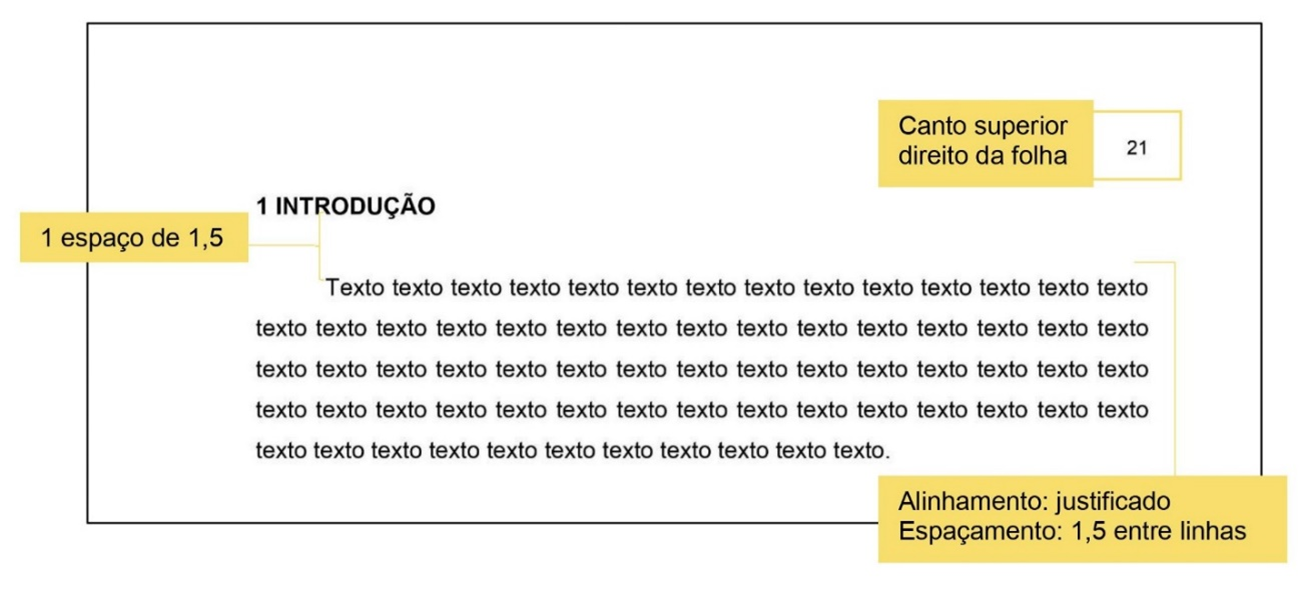
\includegraphics[scale=1]{Textuais/Picture1.png}
% 	\fonte{Elaborada pelos autores (2020), com base na NBR 14724 (2011).}
% \end{figure}


% \subsubsubsection{Seção quinaria}



% O vídeo fornece uma maneira poderosa de ajudá-lo a provar seu argumento. Ao clicar em Vídeo Online, você pode colar o código de inserção do vídeo que deseja adicionar. Você também pode digitar uma palavra-chave para pesquisar online o vídeo mais adequado ao seu documento. Para dar ao documento uma aparência profissional, o Word\footnote{O Microsoft Word é um processador de texto produzido pela Microsoft Office foi criado por Richard Brodie para computadores IBM PC com o sistema operacional DOS em 1983.} fornece designs de cabeçalho, rodapé, folha de rosto e caixa de texto que se complementam entre si. Por exemplo, você pode adicionar uma folha de rosto, um cabeçalho e uma barra lateral correspondentes.

% \begin{table}[!htbp]
% 	\centering
% 	%	\small
% 	\renewcommand{\arraystretch}{1.1}
% 	\caption{Modelo de tabela.}%
% 	\label{tab:tabela_exemplo}
% 	\begin{tabular}{ L{4cm}  R{3cm} || L{4cm}  R{3cm}  }
% 		\hline
% 		Município		& População Estimada & Município		& População Estimada 		\\ 
% 		\hline
% 		Abdon Batista		& 2630	& Bom Jesus				& 2821 \\ 
% 		Abelardo Luz		& 17717	& Bom Jesus do Oeste	& 2156 \\ 
% 		Agrolândia			& 10272	& Bom Retiro			& 9598 \\ 
% 		Agronômica			& 5306	& Bombinhas				& 17477 \\ 
% 		Água Doce			& 7132	& Botuverá				& 4943 \\ 
% 		Águas de Chapecó	& 6379	& Braço do Norte		& 31765 \\ 
% 		\hline
% 	\end{tabular}
% 	\vspace{2mm}
% 	\fonte{Adaptado de IBGE (2015).}
% \end{table}

% Clique em Inserir e escolha os elementos desejados nas diferentes galerias.

% \begin{figure}
% 	\centering
% 	\caption{População.}
% 	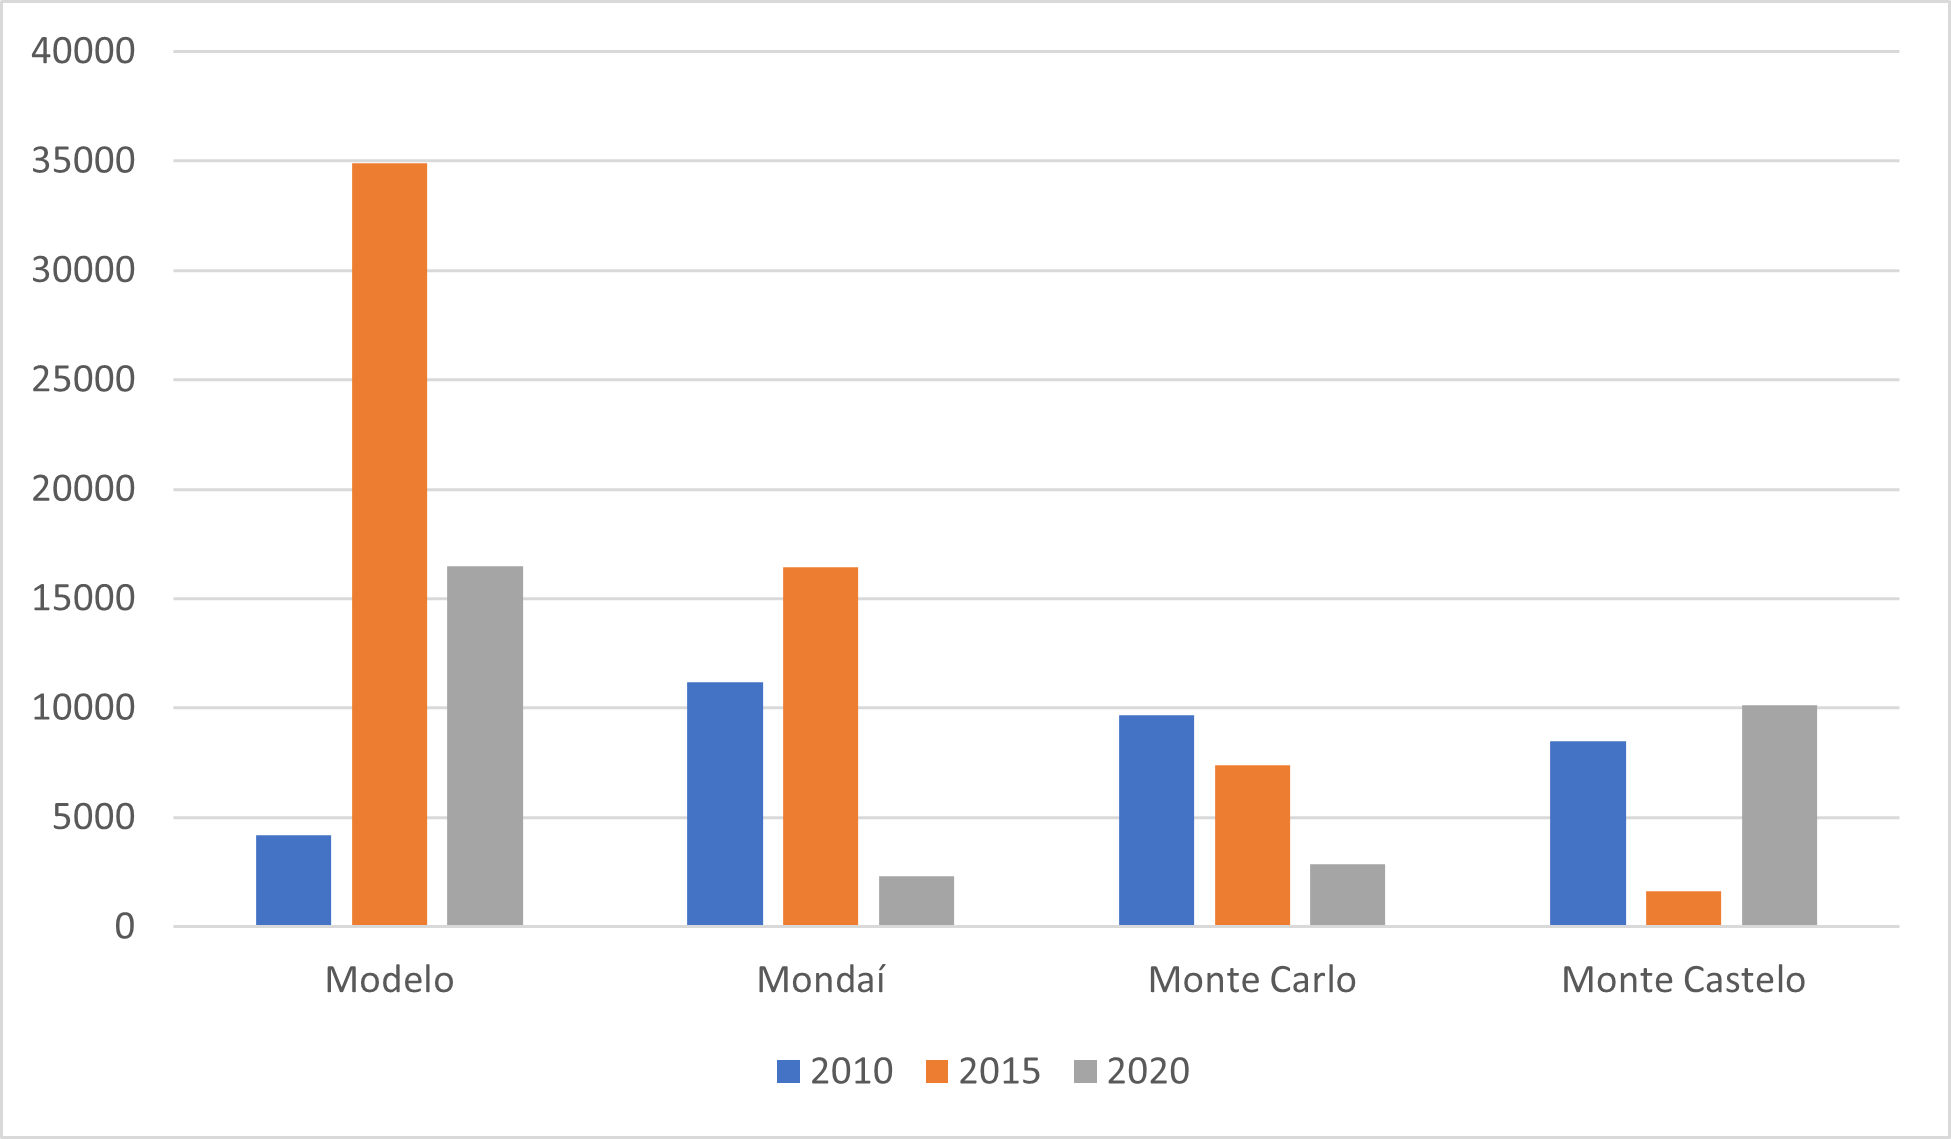
\includegraphics[scale=1]{Textuais/Picture2.png}
% 	\fonte{\me{2020}}
% \end{figure}

% As chamadas às equações e fórmulas, no texto, devem ser feitas da seguinte forma: equação (1), fórmula (2).

% \textbf{Exemplo 1:}
% O Teorema de Pitágoras, é uma equação \eqref{eq:eq1} que pode ser aplicada em qualquer triângulo retângulo (triângulo que tem um ângulo de 90°).
% \begin{equation} \label{eq:eq1}
% a^2 + b^2 = c^2 
% \end{equation}

% \textbf{Exemplo 2:}
% A dopamina é um composto orgânico de função mista álcool, fenol e amina que apresenta fórmula \eqref{eq:form1} molecular:
% \begin{equation} \label{eq:form1}
% \ch{C8 + H11NO2} 
% \end{equation}

% \textbf{Exemplo 3:}
% O modelo matemático de Huang (HUG), dado pelas equações \eqref{eq:eq3} e \eqref{eq:eq4}, foi elaborado com o intuito de fornecer uma descrição mais simples do crescimento bacteriano.
% \begin{gather} 
% 	y(t) = y_0 + y_{max} -\ln{[e^{y_0}  + (e^{y_{max}} -e^{y_0} )  e^{-u_{max}\beta(t)} ]}   \label{eq:eq3}  \\
% 	\beta(t) = t + \frac{1}{4}\ln\left( \frac{1+ e^{-4(t-\lambda)} }{1+ e^{4(\lambda)} }\right) \label{eq:eq4}
% \end{gather}
% \noindent onde $y(t)$ corresponde ao logaritmo natural da concentração celular (log UFC/g) no instante $t$ (dias), $y_{max}$ é o logaritmo natural da população bacteriana (log UFC/g) final, $y_0$ corresponde ao logaritmo natural da população bacteriana inicial (log UFC/g) e $\beta(t)$ é a função de transição.

% \textbf{Exemplo 4:}
% Para o cálculo da intensidade fórmula \eqref{eq:eq5} de Intensidade-Duração-Frequência apresentada, os valores encontrados seguindo os parâmetros apresentados e como o resultado é dado em mm/h haverá também a sua conversão para m/s.
% \begin{gather} 
% 	i = \frac{K T^m}{(t+b)^n}   \label{eq:eq5}  \\[2ex]
% 		i = \frac{\num{625.58} \cdot 5^{\num{0.171}}  }{(60+\num{8.89})^{\num{0.961}}} \\[2ex]
% 		i = \num{44.222} \cdot \frac{\si{mm}}{\si{h}} \cdot \frac{1\mathrm{m}}{\SI{1000}{mm}} \cdot \frac{\SI{1}{h}}{\SI{3600}{s}} 	
% \end{gather}
% \noindent onde, $i$ é a intensidade média máxima de precipitação, em mm/h; $T$ é o Período de retorno, em anos; $t$ é a duração da chuva, em minutos; $k,m,b,n$ são os parâmetros da equação determinados para cada local.


% As citações diretas com até três linhas ``[...] devem estar contidas entre aspas duplas. As aspas simples são utilizadas para indicar citação no interior da citação.'' (ABNT, 2002, p. 2). Devem apresentar autor, ano e página. Quando a indicação de autor estiver dentro de parênteses, o sobrenome deve ser em letra maiúscula. 


% As citações diretas com mais três linhas ``[...] devem ser destacadas com recuo de 4 cm da margem esquerda, com letra menor que a do texto utilizado e sem as aspas.'' (ABNT, 2002, p. 2). Ou seja, utilizar fonte tamanho 10 para as citações diretas longas, com espaçamentos simples entre linhas. As citações devem ser precedidas e antecedidas por um (1) espaço de 1,5 entrelinhas. 

% \begin{citacao}
% Texto texto texto texto texto texto texto texto texto texto texto texto texto texto texto texto texto texto texto texto texto texto texto texto texto texto texto texto texto texto texto texto texto texto texto texto texto texto texto texto texto texto texto texto texto texto. (SILVA, 2020, p. 21).
% \end{citacao}


% Nas citações indiretas não há necessidade de usar aspas e indicar a página, considerando que é uma paráfrase. Faz-se necessário apresentar o autor e ano.






% \noindent Exemplo referência de livro: \cite{exemplo_livro}

% \noindent Exemplo referência de livro em meio eletrônico: \cite{exemplo_livroe}

% \noindent Exemplo referência de trabalho acadêmico (Dissertação de Mestrado): \cite{exemplo_dissertacao}

% \noindent Exemplo referência de trabalho acadêmico (Tese de Doutorado): \cite{exemplo_tese}

% %\noindent Exemplo referência de artigo: \cite{exemplo_artigo}




% \textbf{Para outras referências ver Manual Udesc}: \url{https://www.udesc.br/bu/manuais}









\chapter{Fundamentação teórica}

\section{Conceitos fundamentais}

\subsection{Definição de combustão e estequiometria}
De acordo com Turns (2013, p. 9), a combustão pode ser descrita como "[...] a oxidação rápida gerando calor, ou ambos, calor e luz; também, a oxidação lenta acompanhada por pequena liberação de calor e sem emissão de luz". Uma definição alternativa é proposta por Rendeiro et al. (2008, p. 29), que define combustão como "[...] uma reação química exotérmica entre um combustível e um comburente, usualmente o oxigênio, para liberar calor e formando como produto um grupo de espécies diferente dos reagentes". 

Um processo de combustão é dito estequiométrico quando a quantidade de oxidante fornecida é exatamente a necessária para promover a combustão completa de certa quantidade de combustível \cite{Turns}. De modo geral, os combustíveis usados em reações de combustão são hidrocarbonetos, e o agente oxidante é o oxigênio. Todavia, a combustão com oxigênio puro só se justifica em casos específicos devido ao alto custo de separar o oxigênio do nitrogênio no ar atmosférico, de forma que a combustão usualmente é modelada considerando a reação ocorrendo com ar atmosférico, composto de aproximadamente 21\% de $\ch{O2}$ e 79\% de $\ch{N2}$ \cite{Amazonia}. Para esse caso, a reação de combustão estequiométrica de um hidrocarboneto genérico $\ch{C}_x \ch{H}_y$ pode ser descrita pela Equação molecular \eqref{eq:combest}.
\begin{equation} \label{eq:combest}
\ch{C}_x \ch{H}_y + a_t(\ch{O2} + 3,76 \ch{N2}) \rightarrow{} x \ch{CO2} + y \ch{H2O} + w \ch{N2}.
\end{equation}

A presença do nitrogênio na reação permite que a temperatura da chama, e consequentemente dos gases de combustão, seja reduzida, evitando danos estruturais aos reatores. Todavia, a altas temperaturas ocorre a dissociação do nitrogênio, o que propicia a formação de $\ch{NO}$, produto prejudicial do ponto de vista ambiental \cite{Amazonia}, como será discutido posteriormente. O princípio da conservação da massa torna possível inferir, da Equação \eqref{eq:combest}, que
\begin{equation}
a_t = x + y/2.
\end{equation}

Esse equilíbrio permite definir um parâmetro chamado fração combustível-ar, Equação \eqref{eq:AF}:
\begin{equation} \label{eq:AF}
F = \left(\frac{F}{A}\right) = \frac{m_f}{m_a} 
\end{equation}

\noindent onde $m_a$ indica a massa de ar e $m_f$ indica a massa de combustível (do inglês \textit{fuel}). No caso da estequiometria a proporção é comumente indicada por $\left(\frac{F}{A}\right)_{s}$ (o subscrito s deriva do inglês \textit{stoichiometric}).
Costa (2020, p. 24) ressalta que "cada combustível possui uma quantidade estequiométrica de oxidante, que pode ser determinada através do balanço de massa atômico entre reagentes e produtos da combustão". Dessa forma, a primeira tarefa ao se avaliar um processo de combustão é determinar a quantidade estequiométrica de oxidante.

Ao se tratar de reações químicas, é importante definir parâmetros relacionados à quantidade de matéria. Um deles é a fração mássica de uma espécie química, que para uma espécie química genérica $i$ é definida pela Equação \eqref{eq:y} \cite{Turns}. Os termos $m_i$ e $m_{tot}$ se referem à massa da espécie química e à massa da mistura, respectivamente.
\begin{equation} \label{eq:y}
Y_{i} = \frac{m_i}{m_{tot}} \left[\frac{kg}{kg_{mistura}}\right].
\end{equation}

A fração molar é definida semelhantemente, dessa vez em função do número de mols da espécie química e da mistura ($N_i$ e $N_{tot}$, respectivamente), como mostra a Equação \eqref{eq:cai}.
\begin{equation} \label{eq:cai}
\chi_{i} = \frac{N_i}{N_{tot}} \left[\frac{kmol}{kmol_{mistura}}\right].
\end{equation}

\subsection{Razão de equivalência}
O modelo estequiométrico de um processo de combustão é o ponto de partida para sua análise; todavia, na maioria das aplicações práticas a proporção de oxidante fornecida ao processo é diferente da estequiométrica. Caso a quantidade de oxidante fornecida à reação seja maior do que a estequiométrica, a mistura é dita pobre em combustível. Analogamente, caso essa quantidade seja menor, a reação é dita rica em combustível \cite{Turns}. Quantitativamente, essa característica é expressa através da razão de equivalência ($\Phi$), definida na Equação \eqref{eq:phi} em função da fração combustível-ar estequiométrica ($F_s)$ e modificada ($F$).
\begin{equation} \label{eq:phi}
\Phi = \frac{F}{F_{s}} .
\end{equation}

Da equação acima constata-se que caso $\Phi > 1$ a mistura é rica, para $\Phi < 1$ a mistura é pobre, e para $\Phi = 1$ a proporção é a estequiométrica. Uma grandeza equivalente à razão de equivalência é o excesso de ar ($\%e$), Equação \eqref{eq:excess}, que indica, em porcentagem, o quanto de ar adicional é inserido no processo.
\begin{equation} \label{eq:excess}
\%e = \left(\frac{1-\Phi}{\Phi}\right)\cdot 100\%.
\end{equation}

Em processos de combustão, buscando-se garantir que todo o combustível seja consumido, os reagentes são usados com misturas pobres (Rendeiro et al. (2008) propõe como referência 3\% de excesso de oxigênio, ou seja, 15\% de excesso de ar). Já em processos distintos, como a gaseificação, onde os produtos desejados são principalmente $\ch{CO}$ e $\ch{H_2}$, o processo ocorre com excesso de combustível, operando com apenas 30\% da quantidade de ar estequiométrica \cite{Amazonia}. Especialmente se o processo desejado for a pirólise, que consiste no aquecimento de um material em atmosfera pobre em oxigênio a fim de se obterem combustíveis sólidos, líquidos ou gasosos, $\Phi$ deve ser muito alto.

\subsection{Entalpia de combustão e poderes caloríficos}
A entalpia de combustão pode ser definida como a diferença entre a entalpia dos produtos e a entalpia dos reagentes quando um processo de combustão completa ocorre a uma temperatura e pressão dadas \cite{Shapiro}. Ou seja, é numericamente igual ao calor liberado por um reator no qual ocorre um processo de combustão completo onde os produtos estão à mesma pressão e temperatura que os reagentes. É dada em função das entalpias dos produtos e dos reagentes da reação ($h_{prod}$ e $h_{reag}$, respectivamente):
\begin{equation} \label{eq:entcomb}
\Delta h_R = h_{prod} - h_{reag}.
\end{equation}

\noindent Tendo em vista que $h_{prod}$ é menor que $h_{reag}$, a entalpia de combustão é um valor negativo, e usualmente é dada em $kJ/kg_{comb}$.

O poder calorífico de um combustível é o valor em módulo da entalpia de combustão \cite{Shapiro}. Essa métrica indica a máxima quantidade de calor possível de ser extraída de uma certa massa de combustível. O poder calorífico superior (PCS) é o calor de combustão calculado supondo que a água proveniente da reação foi condensada; já o poder calorífico inferior (PCI) supõe que a água esteja no estado gasoso após a combustão \cite{Turns}. Como a condensação da água é um processo exotérmico, mais energia estará disponível, o que torna o PCS numericamente superior ao PCI. Entretanto, usualmente é o PCI que é usado para a caracterização do combustível.

A partir do PCI é possível definir a potência de um processo de combustão cujo fornecimento de combustível seja constante, a uma vazão mássica $\dot{m}_{comb}$, Equação \eqref{eq:Pot}:
\begin{equation} \label{eq:Pot}
P = \dot{m}_{comb} \cdot PCI.    
\end{equation}


\subsection{Eficiências associadas a processos de combustão}
A eficiência térmica é definida como sendo a razão entre a energia pretendida e a energia gasta. Considerando um processo de combustão, esta eficiência pode ser definida através da Equação \eqref{eq:efcomb} \cite{Turns}. O termo $\dot{Q}_{comb}$ indica o calor disponível na reação e $\dot{m}_{comb}$ é a vazão mássica de combustível.
\begin{equation} \label{eq:efcomb}
\eta_{c} = \frac{\dot{Q}_{comb}}{\dot{m}_{comb}\cdot PCI},
\end{equation}

A eficiência de combustão também pode ser definida em termos de outros parâmetros. Kirch et al. (2018), por exemplo, definem uma eficiência de combustão nominal, em termos de parâmetros relacionados a emissões de poluentes, frequentemente usada no caso de reatores de massa fixa empregados domesticamente. Essa eficiência, chamada pelos autores de NCE (\textit{nominal combustion efficiency}) é definida na Equação \eqref{eq:efcombn}, onde $\chi_{\ch{CO2}}$ e $\chi_{\ch{CO}}$ são as frações molares de dióxido e monóxido de carbono, respectivamente. 
\begin{equation} \label{eq:efcombn}
NCE = \frac{\chi_{\ch{CO2}}}{\chi_{\ch{CO2}} + \chi_{\ch{CO}}},
\end{equation}

\subsection{Biomassa e formação de poluentes}
A biomassa pode ser definida como um material de origem orgânica no estado vivo ou morto, bem como seus respectivos produtos e resíduos \cite{Spliethoff}. Se trata de uma fonte de energia renovável, tendo em vista que sua reposição pela natureza é muito mais rápida do que seu consumo \cite{Brand}. A biomassa a ser tratada no presente trabalho é a florestal, proveniente de resíduos de madeira proveniente de reflorestamento, que posteriormente passam por um processo de peletização.

Em termos de composição, comumente a biomassa lignocelulósica apresenta os elementos C, H, O, N e S (embora a presença de enxofre usualmente é tão baixa que pode ser desprezada). Dessa forma, o processo de combustão estequiométrico apresentado na Equação  \eqref{eq:combest} para a biomassa é melhor descrito através da Equação química \eqref{eq:combestbio}. Os coeficientes da reação química são determinados com base em um balanço de massa. 
\begin{equation} \label{eq:combestbio}
\ch{C} \ch{H}_a \ch{O}_b \ch{N}_c \ch{S}_d + a_t(\ch{O2} + 3,76 \ch{N2}) \rightarrow{} x \ch{CO2} + y \ch{H2O} + z \ch{SO2} + w \ch{N2}.
\end{equation}

No caso de uma reação com excesso ou falta de ar, os produtos da combustão variam, sendo formados compostos intermediários tais como $\ch{CO}$, $\ch{SO_{x}}$ ($\ch{SO} + \ch{SO2}$), $\ch{NO_{x}}$ ($\ch{NO} + \ch{NO2}$), hidrocarbonetos (principalmente $\ch{CH4}$, $\ch{C2H4}$, $\ch{C2H6}$), dentre outros em mais baixa concentração \cite{Lora}. Essa variação pode ocorrer inclusive em uma combustão estequiométrica, tendo em vista que, na prática, a distribuição de ar e combustível não é uniforme dentro do reator. Os poluentes são usualmente classificados em três categorias \cite{Amazonia}:
\begin{enumerate}[noitemsep,nosep,labelindent=\parindent,leftmargin=*,label={\alph*}) ] 
	\item gases que provocam efeito estufa: $\ch{CO2}$ e hidrocarbonetos;
	\item gases nocivos à saúde: $\ch{CO}$, $\ch{SO_{x}}$, $\ch{NO_{x}}$;
	\item resíduos inertes: carbono fixo residual e cinzas.
\end{enumerate}

Dentre os citados acima, os poluentes mais prejudiciais são os produtos que contêm enxofre e nitrogênio. Compostos sulfurados, além de promoverem corrosão superficial dos equipamentos, dão origem à chuva ácida caso sejam lançados na atmosfera. Já os nitrogenados também podem originar chuva ácida, e ao reagirem com o oxigênio produzem ozônio (\ch{O3}), prejudicial em baixas altitudes \cite{Amazonia}. O monóxido de carbono (\ch{CO}) é nocivo à saúde humana tendo em vista que, ao se combinar com a hemoglobina do sangue, impede a absorção de oxigênio, o que pode levar inclusive à morte.

Como já mencionado, tipicamente a biomassa lignocelulósica possui teores de enxofre tão baixos que usualmente sua presença é desprezada. Todavia, a presença de nitrogênio muitas vezes é relevante, como será visto a seguir. Nesse contexto, diversos autores investigam maneiras mais eficazes de converter a biomassa em energia, combinando diferentes processos a fim de maximizar a energia produzida mantendo a emissão de poluentes mínima. No presente trabalho a ênfase é dada em reatores que combinam gaseificação e queima, cujas emissões de $\ch{CO}$, material particulado e $\ch{NO_{x}}$ são reduzidas \cite{Kirch2018}.

%%%%%%%%%%%%%%%%%%%%%%%%%%%%%%%%%%%%%%%%%%%%%%%%%%%%%%%%%%%%%%%%%%%%%%%%%%%%
\section{Processos para conversão da biomassa em energia}
A biomassa pode ser convertida em energia de variadas maneiras, sendo os processos mais empregados a conversão térmica, bio-química e química. Dentre os processos térmicos, ganham destaque a gaseificação e a pirólise; os processos bio-químicos são a fermentação e digestão anaeróbia; e como processo somente químico é destacada a transesterificação \cite{Singh}. A Figura \ref{fig:Pic_biomass} mostra de maneira concisa os referidos processos.

\begin{figure}[!ht]
	\centering
	\caption{Processos de conversão de biomassa em energia.}
	\frame{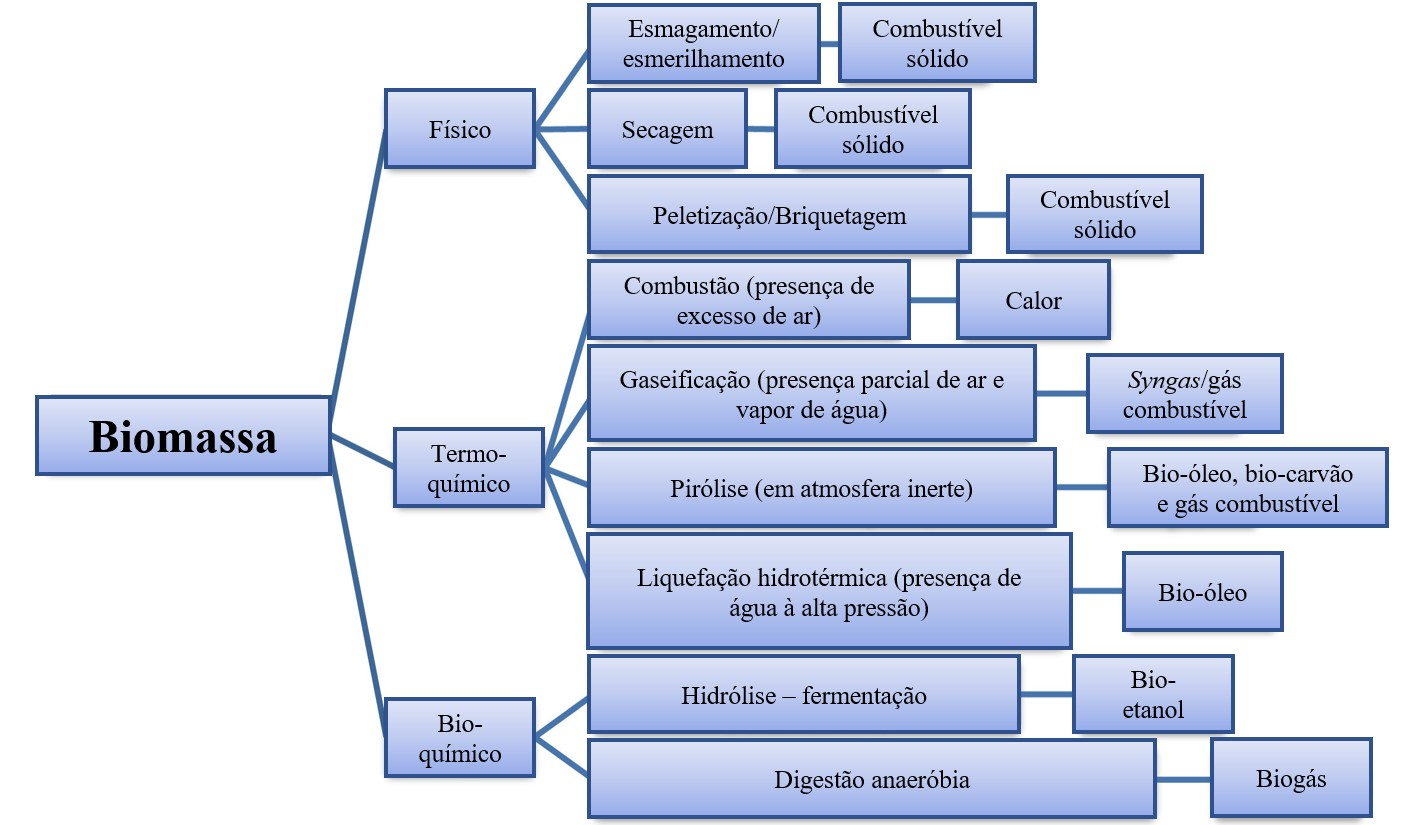
\includegraphics[scale=0.35]{Textuais/Pic_biomass.jpg}}
	\fonte{Adaptado de Sharma, Pareek, Zhang (2015).}
	\label{fig:Pic_biomass}
\end{figure}

A seguir serão apresentados e discutidos os processos térmicos e a queima direta. 

\subsection{Queima direta}
A queima direta, ou incineração, consiste no processo de combustão com a presença de ar em excesso. Para a queima direta da biomassa são necessários grandes volumes de ar atmosférico, e os produtos da reação são basicamente gás carbônico e vapor de água. A energia liberada no processo é o produto de interesse, podendo ser usada para a geração de vapor, que movimentará turbinas e permitirá a geração de energia elétrica \cite{Kretti}, ou somente a fim de produzir calor.

Nos processos de combustão de biomassa, podem ser formadas pequenas quantidades de monóxido de carbono, hidrocarbonetos e demais gases não desejados, tendo em vista que parte do carbono e hidrogênio não reagem completamente com o oxigênio \cite{Brand}. O processo também gera resíduos na forma de cinzas, que não participam da combustão, ainda que no caso de pellets de madeira o teor de cinzas seja geralmente baixo \cite{Spliethoff}. A decomposição da biomassa no caso da combustão se dá em uma sequência de etapas, sendo elas a secagem, pirólise/gaseificação, ignição dos voláteis e combustão do carbono fixo \cite{Brand}.

Dentre os processos térmicos para produção de energia elétrica por meio da biomassa, a combustão é um processo comercial já consolidado, diferentemente da gaseificação, que ainda espera por uma aceitação do mercado como uma possibilidade de produção de biocombustíveis sintéticos \cite{Neves2017}. Por outro lado, muitas vezes o alto teor de umidade da biomassa bruta prejudica a estabilidade da combustão, sendo necessário o estudo de outros processos de conversão ou tratamentos para a biomassa anteriores à combustão \cite{Yaman2004}.

\subsection{Pirólise}
A pirólise é definida por Singh et al. (2010, p. 1373, tradução nossa) como "mudanças químicas que ocorrem quando calor é aplicado a um material na ausência de oxigênio". É um processo que não somente pode ser aplicado à biomassa, mas a diversos outros materiais, a fim de gerar energia. A pirólise é um dos poucos processos que permite que um combustível líquido seja produzido a partir da biomassa \cite{Basu}.

De maneira geral a pirólise de um hidrocarboneto genérico pode ser descrita pela Equação química \eqref{eq:pirolise}:
\begin{equation} \label{eq:pirolise}
\ch{C}_n \ch{H}_m \ch{O}_p + calor \rightarrow{} \sum_{liquido} \ch{C}_a \ch{H}_b \ch{O}_c + \sum_{gas} \ch{C}_x \ch{H}_y \ch{O}_z + \sum_{solido} \ch{C}
\end{equation}

Os produtos da pirólise da biomassa são um sólido de alto teor de carbono, conhecido como coque (ou bio-carvão, ou ainda carbono fixo), e uma fração de voláteis (gases e vapores). Os vapores podem ser condensados gerando um líquido conhecido como bio-óleo ou líquido pirolenhoso, composto de ácido acético, metanol, alcatrão solúvel e insolúvel, etc. \cite{Brand}. Esse líquido pode ser armazenado e usado para produção de energia; já o gás resultante pode ser usado para fornecer energia ao próprio reator \cite{Sharma2015}. É composto principalmente por gases não condensáveis, como $\ch{CO2}, \ch{CO}, \ch{N2}, \ch{H2}$ e hidrocarbonetos \cite{Brand}. 

Os produtos resultantes da pirólise da biomassa dependem da maneira como o processo ocorre. Por exemplo, no caso da pirólise rápida a alta temperatura, o produto em maior quantidade será gás; em contraponto, caso deseje-se maior teor de líquidos, o processo deve ocorrer a menores temperaturas, com alta taxa de fornecimento de calor e com baixo tempo de residência de gás no processo \cite{Singh}. De acordo com Di Blasi apud Sharma et al. (2015, p. 1083, tradução nossa), "Um dos benefícios significativos da pirólise é que é possível conduzi-la em temperaturas mais baixas (normalmente no intervalo de 673-973 K) do que as requeridas nos processos de gaseificação (> 973 K) e combustão (> 1173 K)".

\subsection{Gaseificação}

A gaseificação é constituída por uma série de etapas sequenciais que buscam transformar a nível termoquímico um material sólido ou líquido em um gás sintético. O produto resultante é um gás composto predominantemente por $\ch{H2}$, CO, $\ch{CO2}$, $\ch{N2}$, $\ch{CH4}$ e, em menor quantidade, hidrocarbonetos e demais contaminantes \cite{Nagafugi}, sendo referido usualmente na literatura como gás de síntese, ou \textit{syngas}. O processo ocorre na presença de um agente gaseificante, que pode ser ar, oxigênio, vapor de água ou uma mistura desses componentes, a altas temperaturas (entre 500 e 1400°C); pode também ser realizado a pressão atmosférica ou a altas pressões (até 33 bar). O nível de oxigênio do ambiente é baixo durante o processo, fator que limita a formação de compostos nitrogenados e sulfurados, $\ch{NO}_x$ e $\ch{SO}_x$ respectivamente \cite{Ismail2019}.

O gás resultante no processo pode ser usado diretamente como combustível, sendo oxidado no próprio reator ou armazenado para processo posterior, ou servir de matéria prima para a síntese de produtos químicos. Duas alternativas são possíveis para a biomassa: gaseificá-la diretamente ou convertê-la em carvão vegetal e gaseificar o carvão, sendo que cada um possui vantagens e desvantagens \cite{Brand}.

Em termos de processo, quatro etapas principais ocorrem em reatores de gaseificação, sendo elas a secagem, pirólise, combustão e redução. Na secagem ocorre a evaporação da água contida no combustível (umidade) devido ao aumento da temperatura. A pirólise é a fase em que os gases inflamáveis contidos no sólido são liberados, mediante alta temperatura, sendo que esses gases se misturam com o oxigênio do ar para formar misturas inflamáveis. A combustão é a reação do carbono com o oxigênio, sendo esse um processo exotérmico cuja principal função é fornecer energia para os demais processos ocorrerem. A redução é o processo de gaseificação propriamente dito, onde o carbono sólido se transforma em carbono gasoso através de reações endotérmicas \cite{Amazonia}. A zona onde cada reação ocorre depende do tipo de gaseificador que está sendo usado \cite{Kretti}, sendo que a classificação dos reatores será abordada posteriormente nesse trabalho.

As reações de redução do carbono (quando inicialmente na forma de carvão vegetal) são mostradas nas Equações moleculares abaixo:
\begin{gather} 
	\ch{C} + \ch{CO2} \rightarrow{} 2\ch{CO}   \label{eq:gas1};  \\
	\ch{C} + \ch{H2O} \rightarrow{} 2\ch{CO} + \ch{H2} \label{eq:gas2}; \\
	\ch{C} + 2\ch{H2} \rightarrow{} \ch{CH4} \label{eq:gas3}; \\
	\ch{CH4} + 2\ch{H2O} \rightarrow{} \ch{CO} + 3\ch{H2O} \label{eq:gas4}.
\end{gather}

Barata (2014) ressalta que a gaseificação apresenta-se como um processo mais limpo, tendo em vista que os sólidos residuais do processo (principalmente as cinzas) permanecem dentro do reator, o que diminui a emissão de particulados. Entretanto, para que o gás possa atender aos requisitos de uso, ele deve ser tratado adequadamente. Por exemplo, para uso em turbinas e sistemas de geração de eletricidade, o gás deve estar livre de particulados, alcatrão, compostos de enxofre, cloro e de metais alcalinos. Constitui exceção o caso em que os gases gerados são queimados em sistemas acoplados de gaseificação-combustão, no qual não é necessário tratamento \cite{Brand}. De modo geral, a eficiência do processo é bem alta; se analisada a eficiência como sendo a energia dos gases gerados em relação ao conteúdo da matéria prima, valores típicos obtidos são de 80 a 85\% \cite{Brand}.

Basu (2010, p. 70, tradução nossa) enfatiza que a pirólise "não possui qualquer similaridade com o processo de gaseificação, este envolvendo reações químicas com um agente gaseificante externo conhecido como meio de gaseificação". Os processos diferem também em termos da temperatura, sendo que a pirólise tipicamente ocorre em uma faixa de 300 a 650°C, enquanto a gaseificação ocorre entre 800 e 1000°C \cite{Basu}.

%%%%%%%%%%%%%%%%%%%%%%%%%%%%%%%%%%%%%%%%%%%%%%%%%%%%%%%%%%%%%%%%%%%%%%%%%%%%
\section{Composição e caracterização da biomassa}
Na biomassa lignocelulósica, proveniente da madeira, plantas e folhas, as três macromoléculas em maior quantidades são a hemicelulose, celulose e lignina, sendo que as duas primeiras formam as fibras de madeira e a última mantêm as fibras juntas \cite{Amazonia}. Além de carbono, hidrogênio, oxigênio e nitrogênio, também são encontrados na biomassa resquícios de cálcio, potássio, silício, magnésio, alumínio, enxofre, dentre outros \cite{Febrero2015}. Uma das vantagens da biomassa lignocelulósica é que, diferentemente do amido ou dos carboidratos, a celulose não participa da dieta humana, e seu uso portanto não ameaça a produção de alimentos para consumo humano \cite{Basu}.

Um dos parâmetros fundamentais relativos a biomassa é o teor de umidade ($\omega_{bu}$), que expressa a massa de água contida na biomassa ($m_{\ch{H2O}}$), podendo ser definido pela Equação \eqref{eq:baseumida} no caso de base úmida (quando a massa de água é incluída na massa total, denotada por \textit{bu}). Na Equação, $m_{bio seca}$ se refere à massa de biomassa seca.
\begin{equation} \label{eq:baseumida}
\omega_{bu} = \frac{m_{\ch{H2O}}}{m_{\ch{H2O}}+m_{bio seca}}.
\end{equation}

\noindent Essa quantia pode também ser expressa em base seca (bs), ou seja, o termo $m_{\ch{H2O}}$ é nulo no denominador da Equação \eqref{eq:baseumida}. A título de comparação, o teor de umidade para toras de madeira deixadas ao tempo é de 40 a 55\% bu , já para madeiras secas esse teor cai para uma faixa de 8 a 12\% bu. Sena (2021, p. 18) ressalta que "quanto menor o teor de umidade, maior é a produção de calor por unidade de massa". Entretanto, um teor de umidade inferior a 8\% bu é prejudicial à estrutura da biomassa, pois nesse caso inicia-se um processo de decomposição das estruturas moleculares da madeira \cite{Amazonia}. Além disso, uma biomassa com teor de umidade muito baixo torna o processo de peletização mais difícil, pois propicia uma queima superficial indesejada \cite{Sena2021}.

Outro parâmetro relevante na caracterização da biomassa é a massa específica. Quando se trata de biomassa não contínua, como é o caso de pellets de madeira, é mais conveniente definir uma massa específica aparente (também chamada de densidade a granel, Equação \eqref{eq:rho}). V denota o volume do recipiente usado para determinação do parâmetro. 
\begin{equation} \label{eq:rho}
\omega_{\rho_{ap}} = \frac{m_{biomassa}}{V}.
\end{equation}

\noindent Essa medida é dita aparente pois existem espaços não preenchidos entre os pellets, tornando a medida menor do que a massa específica real \cite{Amazonia}. A massa específica aparente é um parâmetro muito relacionado à logística, pois quanto maior essa propriedade, mais quantidade de massa pode ser transportada em um mesmo volume, tornando o processo mais viável economicamente \cite{Sena2021}.

Algumas características da biomassa são determinadas com base na chamada análise imediata, sendo elas o teor de voláteis, cinzas e carbono fixo \cite{Basu}. O teor de materiais voláteis é definido como a quantidade de componentes que podem ser removidos por efeito somente da temperatura em atmosfera inerte ou não oxidante \cite{Sena2021}. O teor de voláteis na biomassa de madeira é geralmente alto, variando entre 76 e 86\% bs \cite{Obernberger2004}. Já o teor de cinzas quantifica a quantidade de resíduos sólidos que sobram após a queima completa do combustível. As cinzas são compostas principalmente de óxidos minerais, e também fazem parte da sua composição possíveis resquícios de poeira, terra etc. \cite{Sena2021}. Obernberger et al. (2004) cita que, para biomassa de madeira densificada, o teor de cinzas geralmente situa-se entre 0,4 e 1,3\% bs. 

A caracterização de biomassa proveniente de madeira é realizada com base nas normas da ASTM (\textit{American Society for Testing and Materials}). Vale ressaltar que a norma brasileira mais próxima para se caracterizar combustíveis de origem lignocelulósica foi a NBR 8112, usada para caracterização de carvão vegetal; todavia a norma foi cancelada no ano de 2015. As principais normas de ensaio para obtenção da análise imediata de combustíveis provenientes da madeira são relacionados por Basu (2010):
\begin{enumerate}[noitemsep,nosep,labelindent=\parindent,leftmargin=*,label={\alph*}) ] 
	\item teor de voláteis: ASTM E-872;
	\item teor de cinzas: ASTM D-1102;
	\item teor de umidade: ASTM E-871;
	\item teor de carbono fixo: obtido pela diferença. 
\end{enumerate}

Alternativamente, a análise imediata pode ser realizada através de análise termogravimétrica. Nessa técnica, uma amostra de combustível sólido é aquecida em atmosfera específica em uma microbalança eletrônica. A variação de massa do combustível, indicada por um dispositivo específico de termogravimetria, permite determinar os teores de umidade, materiais voláteis e teor de cinzas \cite{Basu}.  

A composição em termos dos elementos básicos é determinada pela análise elementar, sendo a composição do combustível então descrita em termos do teor de C, H, O, N, S, cinzas e umidade. Se trata de uma análise relativamente mais cara e complicada, se comparada à análise imediata \cite{Basu}. Basu (2010) menciona as normas ASTM E-777, E-778, E-775 para determinação do teor de carbono e hidrogênio, nitrogênio e enxofre, respectivamente, para biomassa proveniente de refugo. O teor de umidade e cinzas é determinado de acordo com as normas já mencionadas anteriormente. A Tabela \ref{tab:elementar} relaciona características de diversos tipos de biomassa, bem como suas principais propriedades. 

\begin{table}[!htbp]
	\centering
	\small
	\renewcommand{\arraystretch}{1.3}
	\caption{Composição elementar de alguns tipos de biomassa.}%
	\label{tab:elementar}
	\begin{tabular}{|l|l|l|l|l|l|l|l|}
    	\hline
        \textbf{Biomassa}    & \textbf{C (\%)} & \textbf{H (\%)} & \textbf{O (\%)} & \textbf{N (\%)} & \textbf{S (\%)} & \textbf{Cinzas (\%)} & \textbf{Fonte}      \\
        \hline
        Plátano              & 50,6            & 6,0             & 41,7            & 0,3             & 0               & 1,4                  & Basu (2010)         \\
        \hline
        Cascas de arroz      & 39,2            & 5,1             & 35,8            & 0,6             & 0,1             & 19,2                 & Basu (2010)         \\
        \hline
        Serragem             & 47,2            & 6,5             & 45,4            & 0               & 0               & 1,0                  & Basu (2010)         \\
        \hline
        Eucalipto         & 46,3±0,5        & 6,4±0,1         & 46,8±0,6        & 0,1±0,0         & -               & 0,4±0,0              & Neves et al. (2017) \\
        \hline
        Pinus             & 48,0±1,2        & 6,3±0,1         & 45,1±1,2        & 0,1±0,0         & -               & 0,5±0,0              & Neves et al. (2017) \\
        \hline
        Pellets   & 49,1±1,0        & 6,6±0,1         & 43,5±1,1        & 0,1±0,0         & -               & 0,7±0,0              & Neves et al. (2017) \\
        \hline
        
    \end{tabular}

	\vspace{2mm}
	\fonte{O autor.}
\end{table}

%Outra propriedade que permite caracterizar a biomassa é o PCI. Os fatores que mais influenciam o poder calorífico da biomassa lignocelulósica são a composição química, tipo, teor de umidade e teor de cinzas. Brand (2010) destaca que espécies de plantas gimnospermas (coníferas) de maneira geral possuem poder calorífico maior do que angiospermas. Um maior teor de umidade também implica em um menor poder calorífico líquido; da mesma forma, quanto maior o teor de cinzas, menor é o PCI, tendo em vista que as cinzas não participam das reações \cite{Brand}. 

\subsection{Peletização}
Dentre os processos de adensamento da biomassa lignocelulósica, um dos mais importantes é a peletização (do inglês \textit{pelletization}). O processo permite o aumento da densidade energética do combustível, bem como facilita o transporte e armazenamento. Outras vantagens dos pellets são seu alto poder calorífico, fácil ignição, além de possuírem baixo teor de cinzas e enxofre \cite{Lin2021}. 

O processo de peletização é realizado através de uma prensa, que realiza pressão sobre a biomassa moída e força-a a passar sobre uma matriz com perfurações circulares. O resultado são pequenos cilindros, de diâmetro entre 5 e 15 mm e massa específica que geralmente se situa na faixa de 1000 e 1300 kg/m³ \cite{Amazonia}. Geralmente não é necessária a adição dos chamados ligantes, pois a própria lignina passa por um processo de plasticização ao ser submetida às temperaturas da peletizadora, atuando então como um aglutinante natural \cite{Sena2021}.

\subsection{Efeitos de composição}
%O poder calorífico da biomassa é bastante relacionado à sua composição, bem como o modo de densificação utilizado (peletização, briquetes etc.) \cite{Spliethoff}. O mesmo autor indica o valor de poder calorífico de pellets de palha como sendo 14,4 MJ/kg. 
Os fatores que mais influenciam o poder calorífico da biomassa lignocelulósica são a composição química, tipo, teor de umidade e teor de cinzas. Brand (2010) destaca que espécies de plantas gimnospermas (coníferas) de maneira geral possuem poder calorífico maior do que angiospermas. Um maior teor de umidade também implica em um menor poder calorífico líquido; da mesma forma, quanto maior o teor de cinzas, menor é o PCI, tendo em vista que as cinzas não participam das reações \cite{Brand}. Spliethoff (2010) traz um gráfico que relaciona o poder calorífico inferior de alguns tipos de biomassa como função do teor de umidade, mostrado na Figura \ref{fig:PCIw}. O autor também cita que o PCI da biomassa lignocelulósica seca e sem cinzas situa-se na faixa entre 17 e 21 MJ/kg.
\begin{figure}
	\centering
	\caption{PCI como função da umidade para palha (\textit{straw}) e madeira (\textit{wood}).}
	\frame{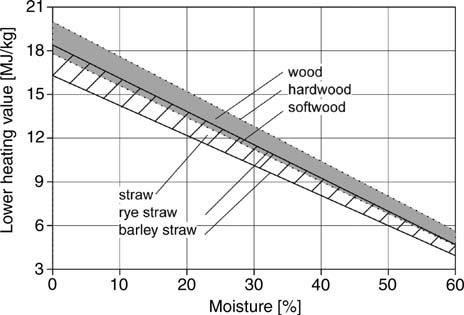
\includegraphics[scale=0.7]{Textuais/Pictures/moistureLHV.png}}
	\fonte{Spliethoff (2010).}
	\label{fig:PCIw}
\end{figure}

Outro ponto em que a biomassa se diferencia em relação aos combustíveis tradicionais, tal como o carvão mineral, é o teor de voláteis. A Figura \ref{fig:volatiles} mostra um gráfico que relaciona o teor de voláteis (\textit{volatiles}), cinzas (\textit{ash}) e carbono fixo (\textit{coke}) para dois tipos de carvão, palha e madeira.

\begin{figure}
	\centering
	\caption{Teores de voláteis, cinzas e carbono fixo para diferentes combustíveis sólidos.}
	\frame{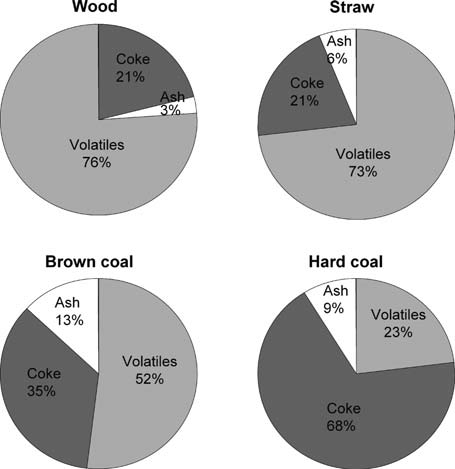
\includegraphics[scale=0.7]{Textuais/Pictures/volatiles.png}}
	\fonte{Spliethoff (2010).}
	\label{fig:volatiles}
\end{figure}

Em relação a composição dos voláteis emitidos pela biomassa, existem diversos estudos, com enfoque principalmente na gaseificação. Neves et al. (2017) avaliam a composição dos voláteis gerados no processo de gaseificação de quatro tipos de pellets em um reator de leito fluidizado. Os testes foram conduzidos para uma faixa de temperatura de 600 a 975°C, sendo a temperatura média do leito 750°C. Os autores mediram a concentração dos gases formados na pirólise em função da temperatura, usando o balanço de massa para verificar a consistência dos dados. Os gases avaliados como produtos da pirólise foram $\ch{H2}, \ch{CO}, \ch{CO2}, \ch{CH4}, \ch{C2H4}$ e $\ch{C2H6}$, sendo $\ch{C3H8}$ também verificado como um produto relevante. Uma das principais conclusões é que a composição do gás resultante é bastante correlacionada à temperatura do processo, sendo que a produção de $\ch{H2}$ e $\ch{CO}$ tem um aumento acentuado com o aumento da temperatura, enquanto para os demais gases verifica-se um pico de produção em uma temperatura intermediária. Essa dependência é semelhante em todos os quatro tipos de pellets testados, à exceção da produção de $\ch{CO}$, que varia conforme o teor de oxigênio do combustível. 

Por fim, outro fator relevante em termos da composição da biomassa é a possibilidade de formação de incrustações no reator. Febrero et al. (2015) analisaram a formação de incrustações em um modelo de pequena escala de um queimador de pellets. Dois elementos críticos nesse aspecto foram o cloro e enxofre, sendo que no caso do combustível em questão o cloro foi o elemento que mais formou incrustações nas superfícies de troca de calor. Os demais elementos residuais analisados permaneceram junto às cinzas, sendo mais facilmente removidos do processo. O estudo também concluiu que o volume de ar injetado no reator deve ser o maior possível, quando o objetivo é evitar incrustações.

\section{Reatores para biomassa}
Dentre os tipos de reatores para processamento de biomassa, ganham destaque os gaseificadores, que proporcionam a formação do gás combustível necessário para o processo de queima. A Figura \ref{fig:gasification_technologies} apresenta um panorama das principais tecnologias de gaseificação.

\begin{figure}[!ht]
	\centering
	\caption{Tecnologias de gaseificação.}
	\frame{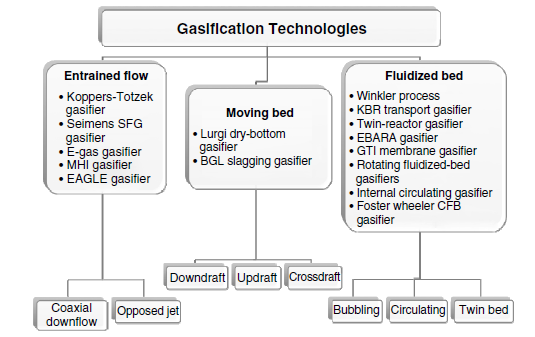
\includegraphics[scale=0.7]{Textuais/gasification_technologies.png}}
	\fonte{Basu (2010).}
	\label{fig:gasification_technologies}
\end{figure}

Ainda, os reatores podem ser classificados de acordo com a alimentação de biomassa, sendo tipos possíveis os de alimentação contínua, intermitente ou por lote (encontrado na literatura como \textit{batch}, onde toda a biomassa é adicionada no início do processo) \cite{Kruger}. Em reatores de combustão para biomassa de leito fixo, como os voláteis se desprendem e são queimados sobre o leito, é conveniente dividir o fluxo de ar em duas partes, um fluxo para a combustão do carbono fixo e outro para a combustão dos voláteis. O objetivo nesse caso é promover a queima completa dos voláteis e do carbono fixo \cite{Brand}.

O reator do presente trabalho se encaixa na categoria \textit{moving bed}, no qual existe uma grade que suporta a biomassa, e o combustível desce conforme vai sendo consumido \cite{Basu}. Essa categoria por sua vez se divide em três outros tipos: \textit{updraft} (contracorrente), \textit{downdraft} (co-corrente), e \textit{crossdraft} (corrente cruzada). A seguir serão detalhados os reatores contracorrente, co-corrente e os reatores multi-estágios, que aliam o processo de volatilização (gaseificação ou pirólise) ao de queima em um mesmo equipamento.

\subsection{Reatores contracorrente}
Nesse tipo de reator o meio de gaseificação, que geralmente é o ar, é inserido pelo fundo do reator e ascende em direção ao topo, enquanto o combustível se move para baixo \cite{Basu}. Uma representação é dada na Figura \ref{fig:updraft}.

\begin{figure}[!ht]
	\centering
	\caption{Esquema de reator do tipo contracorrente, com as principais reações e distribuição de temperaturas.}
	\frame{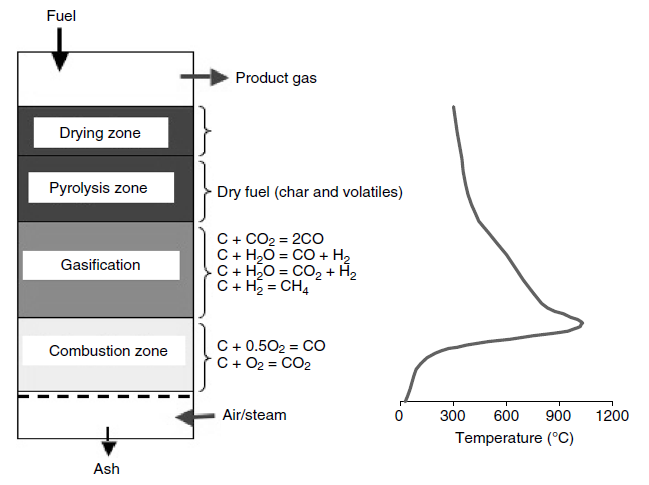
\includegraphics[scale=0.6]{Textuais/updraft.png}}
	\fonte{Basu (2010).}
	\label{fig:updraft}
\end{figure}

Se trata de um reator adequado para biomassa com alto teor de cinzas (até 25\%) e umidade (60\%). São verificadas altas taxas de formação de alcatrão, tornando o reator menos adequado para combustíveis com alto teor de voláteis. Entretanto, é possível queimar o gás logo após sua produção, o que promove a participação do alcatrão na reação. Nesse caso, não é necessária a limpeza do gás, e o uso de combustíveis com teor de voláteis mais alto não se torna um problema \cite{Basu}.

\subsection{Reatores co-corrente}
Diferentemente dos reatores contracorrente, nesse caso o agente gaseificador é inserido apenas na metade do reator e os gases resultantes do processo são retirados pelo fundo. Um esquema desse tipo de reator é mostrado na Figura \ref{fig:downdraft}.

\begin{figure}[!ht]
	\centering
	\caption{Reator do tipo co-corrente.}
	\frame{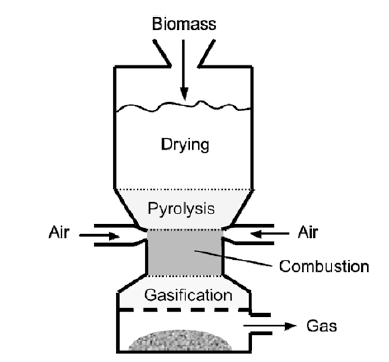
\includegraphics[scale=0.6]{Textuais/downdraft.png}}
	\fonte{Basu (2010).}
	\label{fig:downdraft}
\end{figure}

Primeiramente ocorre a evaporação da água presente na biomassa, e em seguida, sob o efeito do calor produzido na zona de reação e sem existência de oxigênio, ocorre a pirólise. O ar somente é introduzido na metade do reator, onde então ocorre a combustão. Por fim, o gás resultante (produtos da combustão + oxigênio) é direcionado pela camada de carbono fixo formada, gaseificando-a. Os gases podem ser retirados então pelo fundo do reator \cite{Basu}.

Uma das vantagens de um reator desse tipo é o fato de que os gases produzidos passam próximo à camada de cinzas na base, o que favorece reações de craqueamento do alcatrão, gerando um produto com baixo teor desse elemento \cite{Basu}. Esse fator faz com que o gás gerado no processo possa ser diretamente usado em um motor de combustão interna, por exemplo.

%\subsection{Reatores Crossdraft}
%Ver se é necessário falar.

\subsection{Queimador multi-estágios}
Nesse caso o gás gerado no processo de gaseificação é queimado logo após sua formação. Uma das vantagens desse processo é a redução de custos, caso o produto desejado seja somente calor, tendo em vista que o gás combustível produzido por gaseificadores contracorrente possui alto teor de alcatrão. Dessa forma, é necessário um processo de limpeza antes de o gás ser usado em motores ou turbinas, por exemplo. Promovendo a combustão desse gás logo após sua formação, essa limpeza não é necessária \cite{Scharler2011}.

Outra vantagem é em termos de emissão de poluentes. A queima do gás proveniente da gaseificação é propensa a formação de $\ch{NO}_x$, o que pode ser melhorado justamente através da queima em duas etapas \cite{Scharler2011} \cite{Kirch2018}. No mesmo contexto, uma das desvantagens de gaseificadores contracorrente é o alto teor de alcatrão do gás resultante. Todavia, quando o gás produzido é diretamente queimado, o próprio alcatrão acaba se tornando um combustível, beneficiando o processo \cite{Brunner2017}.

\subsection{Modelos de reatores da literatura}

Um modelo de reator cujo foco é unicamente a gaseificação com alimentação contínua de biomassa é proposto por Mandl et al. (2017). Nele, os autores buscam modelar matematicamente um gaseificador de leito fixo contracorrente para operação em regime permanente. Uma representação do reator, onde também são mostrados os processos aos quais os pellets são submetidos, é mostrada na Figura \ref{fig:mandl}.

\begin{figure}[!ht]
	\centering
	\caption{Modelo de gaseificador proposto pelos autores.}
	\frame{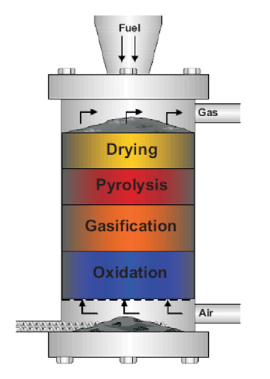
\includegraphics[scale=0.7]{Textuais/burner_mandl.png}}
	\fonte{Mandl, Obernberger, Biedermann (2010).}
	\label{fig:mandl}
\end{figure}

No topo da biomassa o processo dominante é a secagem, onde a água presente nos pellets evapora devido ao calor proveniente dos gases gerados nas etapas posteriores. Em seguida, os pellets passam pelo processo de pirólise, a uma temperatura em torno de 500 K, onde ocorre o desprendimento dos voláteis. A biomassa não volatilizada desce e, devido ao aumento da temperatura (acima de 1000 K), passa pelo processo de gaseificação. Por fim, o combustível restante no reator, que consiste basicamente em carbono fixo, é oxidado pelo ar suprido na parte inferior do reator, processo que fornece energia às demais etapas \cite{Mandl2010}.

Obernberger et al. (2017) desenvolveram um protótipo de reator onde um gaseificador de leito fixo contracorrente é diretamente acoplado a um queimador multi-estágios. O objetivo é promover um processo de baixa emissão de CO, componentes orgânicos e material particulado, tanto para combustíveis convencionais (pellets de madeira e maravalhas) quanto para os menos comuns, como resíduos florestais e resíduos provenientes da agricultura. O esquema do queimador pode ser verificado na Figura \ref{fig:obernberger}.

\begin{figure}[!ht]
	\centering
	\caption{Modelo de reator com gasificação e queima multi-estágios acoplada.}
	\frame{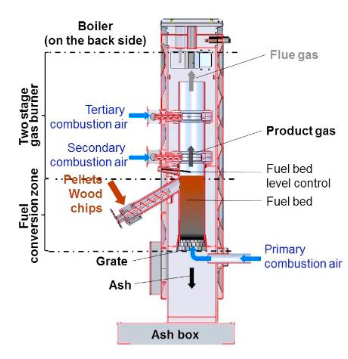
\includegraphics[scale=0.7]{Textuais/burner_obernberger.png}}
	\fonte{Obernberger et al. (2017).}
	\label{fig:obernberger}
\end{figure}

\noindent Os autores concluíram que o queimador apresenta um excelente desempenho em termos de emissão de CO e compostos orgânicos, bem como de particulados. Também foi constatado que o excesso de ar a ser utilizado pode ser baixo, da ordem de 1,2, sem ocorrência de incrustações.

Outro modelo de reator que alia gaseificação e queima é proposto por Pavel et al. (2019), mas diferentemente do anterior, esse modelo não possui alimentação contínua, sendo necessário adicionar toda a massa de combustível a ser usada no início do processo (reator do tipo \textit{batch}). Além disso, só existe uma injeção de ar na etapa de combustão. Uma representação do reator está mostrada na Figura \ref{fig:pavel}.

\begin{figure}[!ht]
	\centering
	\caption{Modelo de reator com gaseificação e queima simultâneas.}
	\frame{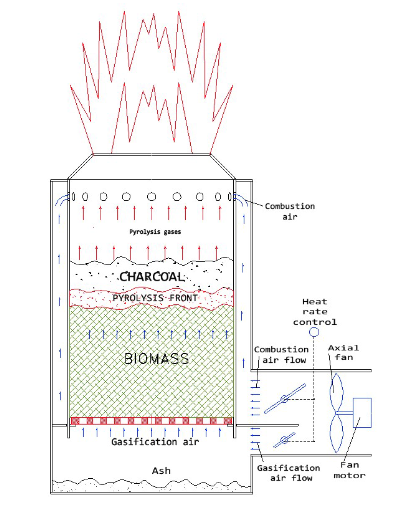
\includegraphics[scale=0.5]{Textuais/burner_pavel.png}}
	\fonte{Pavel et al. (2019).}
	\label{fig:pavel}
\end{figure}

Esse queimador possui a característica de ser do tipo \textit{top-lit}, ou seja, a ignição é feita na superfície superior da biomassa. Ocorre então a formação de uma frente de combustão, que avança em direção ao fundo do reator. O combustível próximo à zona de combustão, devido à ação da temperatura, sofre os processos de secagem e pirólise, ocorrendo então o desprendimento dos voláteis, que são direcionados ao topo do reator para serem oxidados. No momento que a frente de combustão chega ao fundo do reator, existe cerca de 10 a 20\% de carbono fixo restante, sendo esse carbono possível de ser gaseificado e queimado no topo do reator \cite{Pavel2019}.

Semelhantemente, Oberneberger et al. (2011) estudaram um gaseificador de alimentação contínua de pellets, acoplado a uma câmara separada de combustão. Os gases considerados como produtos da gaseificação são o $\ch{CO}$, $\ch{H2}$, $\ch{CO2}$, $\ch{CH4}$, além de vapor de água, nitrogênio, alcatrão e traços de hidrocarbonetos. O conjunto do reator proposto pelos autores possui ao todo três injeções de ar: a primeira injeção se situa no gaseificador, e as outras duas no queimador. A primeira injeção do queimador é dimensionada para promover uma queima pobre, a fim de proporcionar uma zona de redução, inibindo a formação de $\ch{NO}$; a segunda injeção o oxigênio restante necessário é fornecido, a fim de promover a queima completa do gás. O esquema do reator é mostrado na Figura \ref{fig:scharler}.

\begin{figure}[!ht]
	\centering
	\caption{Modelo de reator proposto por Obernberger et al. (2017)}
	\frame{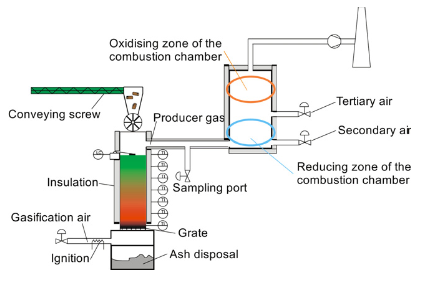
\includegraphics[scale=0.7]{Textuais/queimador_scharler.png}}
	\fonte{Mandl, Obernberger, Scharler (2011).}
	\label{fig:scharler}
\end{figure}

Nos resultados, os autores destacam que as temperaturas na base da cama de pellets (grade) chegam até 1480 K, fator que deve ser levado em conta tendo em vista a ocorrência de fusão das cinzas. Dessa forma, biomassas com ponto de fusão de cinzas muito baixo não devem ser usadas. O tipo de pirólise verificado foi a pirólise lenta, dado que foi obtido com base no tempo de residência dos pellets no reator e na temperatura alcançada. Foi verificado que o gás produzido apresenta alto teor de alcatrão, como previsto por outros autores, o que pode acarretar na condensação desse produto caso o gaseificador não seja bem isolado, especialmente em baixas vazões volumétricas de ar. Por fim, verificou-se que o modelo proposto emite pouco $\ch{CO}$, o que indica uma queima quase total do gás proveniente da gaseificação; quanto às emissões de nitrogênio, os autores verificaram que a concentração de $\ch{NO}$ não mudou significativamente ao longo da zona de redução da câmara de combustão, e que emissões de $\ch{NO}_x$ são mais baixas para uma vazão de ar menor. 


\chapter{Metodologia}

\section{Aparato experimental e combustível}
O protótipo de reator disponibilizado pela Koala Energy consiste em um reator de dois estágios, um de volatilização (inferior) e outro de combustão (superior). O ar atmosférico é injetado no reator por um ventilador centrífugo da fabricante ebm-papst, sendo que, ao entrar no reator, o fluxo de ar se divide em dois: um é direcionado ao fundo do reator, onde passa pela grelha e pela cama de pellets, proporcionando as condições para a gaseificação da biomassa (referido daqui em diante como injeção primária de ar); o segundo fluxo é dirigido aos orifícios na parede interna do queimador, localizados no topo (injeção secundária de ar). Esse último fluxo proporcionará a combustão dos gases gerados no fundo do reator, completando o processo.

Um desenho simplificado do reator é mostrado na Figura \ref{fig:queimador_koala}. O orifício lateral maior é onde há a conexão com o ventilador. A circulação do ar destinado à injeção secundária no interior da parede do reator é vantajosa, tendo em vista que o ar é pré-aquecido nesse processo. Entretanto, o dispositivo não conta com um mecanismo de regulagem de vazão especificamente para as injeções primária e secundária. 

\begin{figure}[!ht]
	\centering
	\caption{Modelo do queimador usado no presente estudo.}
	\frame{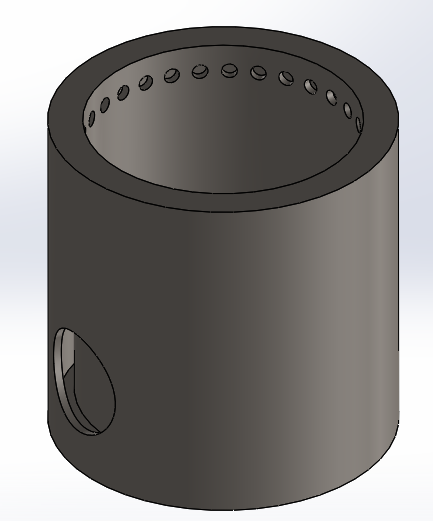
\includegraphics[scale=0.5]{Textuais/experimental/vista_opaca.png}}
	\frame{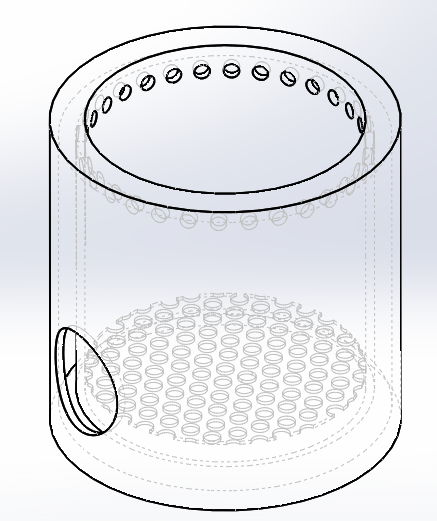
\includegraphics[scale=0.5]{Textuais/experimental/vista_transparente.png}}
	\fonte{O autor (2022).}
	\label{fig:queimador_koala}
\end{figure}

Para permitir um estudo mais completo, a empresa projetou e fabricou um sistema de alimentação automático de combustível, além de uma capela para exaustão de gases. Também foi disponibilizado o sistema de controle elétrico, por meio do qual é possível controlar a vazão de combustível, o acionamento do ventilador do queimador e o sistema de exaustão da capela. O aparato experimental disponibilizado pela empresa é mostrado na Figura \ref{fig:aparatokoala} (imagem obtida antes de serem iniciados os testes).

\begin{figure}
	\centering
	\caption{Aparato experimental disponibilizado pela empresa.}
	\frame{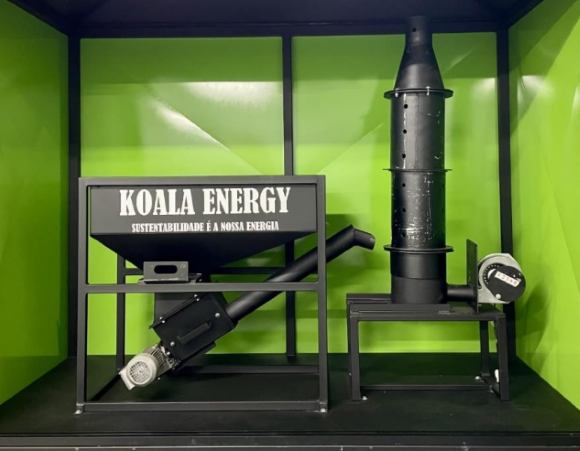
\includegraphics[scale=0.5]{Textuais/experimental/capela.png}}
	\fonte{O autor (2022).}
	\label{fig:aparatokoala}
\end{figure}

O combustível utilizado são pellets de madeira do gênero \textit{pinus}, proveniente de reflorestamento, sendo produzidos a partir de resíduos da indústria de processamento de madeira. O produto possui certificação \textit{ENplus} A1, o mais alto nível na classificação da \textit{ENplus}, órgão de origem europeia voltado a certificação de pellets. A avaliação do instituto é feita com base nas normas ISO, levando em conta as variáveis associadas ao combustível. Na Figura \ref{fig:pellets_koala} são mostrados os pellets produzidos pela empresa.

\begin{figure}[!ht]
	\centering
	\caption{Pellets produzidos pela empresa Koala Energy.}
	\frame{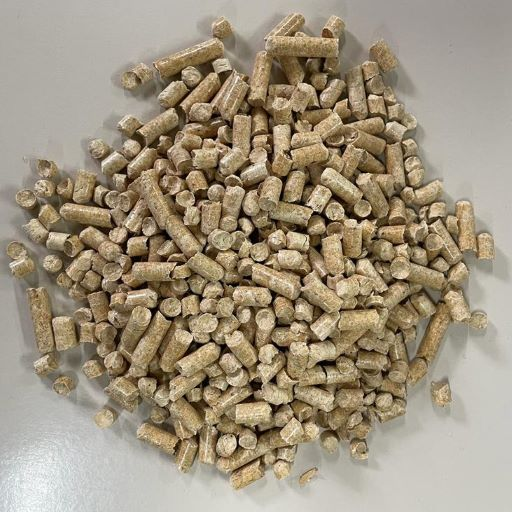
\includegraphics[scale=0.5]{Textuais/experimental/pellets_koala.jpeg}}
	\fonte{O autor (2022).}
	\label{fig:pellets_koala}
\end{figure}

Alguns parâmetros importantes dos pellets, fornecidos pela empresa, são mostrados na Tabela \ref{tab:propriedadespellets}.

\begin{table}[!ht]
	\centering
	\small
	\renewcommand{\arraystretch}{1.3}
	\caption{Algumas propriedades dos pellets da Koala, informados pela empresa.}%
	\label{tab:propriedadespellets}
        \begin{tabular}{|l|c|}
        \hline
        \multicolumn{1}{|c|}{\textbf{Propriedade}} & \textbf{Valor} \\ \hline
        Diâmetro                                   & 6,6 mm         \\ \hline
        Densidade aparente                         & 720 kg/m³      \\ \hline
        Teor de cinzas (a 550°C, bs)               & 0,5\%          \\ \hline
        \multirow{2}{*}{PCI} & 5,11 kWh/kg    \\ \cline{2-2} 
                                                   & 18,40 MJ/kg    \\ \hline
        Teor de enxofre (bs)                       & 0,014\%        \\ \hline
        Teor de nitrogênio (bs)                    & 0,16\%         \\ \hline
        \end{tabular}
	\vspace{2mm}
	\fonte{O autor (2022).}
\end{table}

Outra análise relevante em relação ao combustível é a análise elementar, usada para modelar matematicamente a reação, como será visto adiante. Tendo em vista não ser possível realizar essa análise no Centro de Ciências Tecnológicas da Udesc, não foi possível obter essa análise em tempo hábil para os ensaios. Portanto, foi usada a composição elementar de outra biomassa semelhante como base. A análise escolhida foi a de Neves et al. (2017), anteriormente mostrada na Tabela \ref{tab:elementar}, e novamente na Tabela \ref{tab:elementar_modelagem}. Nesta Tabela, $Y$ representa a fração mássica de cada elemento. 

\begin{table}[!ht]
	\centering
	\small
	\renewcommand{\arraystretch}{1.3}
	\caption{Composição elementar dos pellets usada para obter o modelo matemático.}%
	\label{tab:elementar_modelagem}
        \begin{tabular}{|l|l|l|l|l|l|l|}
        \hline
        \textbf{Elemento} & C    & H   & O    & N   & S & Cinzas \\ \hline
        \textbf{Y (\%)}   & 49,1 & 6,6 & 43,5 & 0,1 & - & 0,7    \\ \hline
        \end{tabular}
	\vspace{2mm}
	\fonte{Adaptada de Neves et al. (2017).}
\end{table}


\section{Variáveis medidas}

\subsection{Temperatura e emissão de poluentes}
Para caracterizar o processo de combustão dos gases gerados no processo de volatilização, as principais métricas necessárias são o perfil de temperatura e emissão de poluentes. Dessa forma, é necessário um dispositivo que permita acoplar os instrumentos de medição ao processo. O dispositivo projetado no laboratório foi uma chaminé, dividida em 3 seções, que possui função tanto no monitoramento da temperatura quanto na avaliação dos poluentes. A representação 3D do conjunto é mostrada na Figura \ref{fig:projeto_chamine}.

\begin{figure}
	\centering
	\caption{Projeto da chaminé para medição de temperatura e emissões.}
	\frame{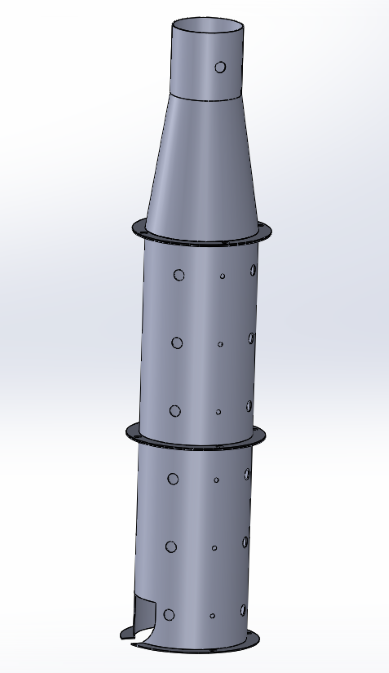
\includegraphics[scale=0.5]{Textuais/experimental/projeto_chamine.png}}
	\fonte{O autor (2022).}
	\label{fig:projeto_chamine}
\end{figure}

A primeira seção (de baixo para cima) possui uma abertura lateral para permitir que o alimentador de pellets seja posicionado corretamente. Os orifícios maiores possibilitam o posicionamento da sonda de gases, enquanto os orifícios menores permitem a inserção dos termopares. O segundo estágio possui função idêntica ao primeiro, enquanto o terceiro permite unicamente a medição de poluentes. Esse último estágio possui um perfil cônico, que permite uma uniformização do fluxo de gases, permitindo uma medição de poluentes final mais adequada. Antes dos testes, a chaminé foi revestida com uma manta térmica de fibra cerâmica, visando reduzir a perda de calor pelas paredes.

Os termopares utilizados são do tipo K, sendo possível posicioná-los a uma distância inicial de 50 mm do reator e após em intervalos regulares de 100 mm entre si. No presente estudo a medição de temperatura foi feita somente em um ponto, sendo o termopar posicionado no orifício de medição de temperatura mais alto da chaminé. O termopar foi conectado ao sistema de aquisição de dados Keysight (Figura \ref{fig:keysight}), que por sua vez é conectado a um computador, permitindo monitorar a temperatura através do software Keysight BenchVue.

\begin{figure}[!ht]
	\centering
	\caption{Sistema de aquisição de dados Keysight e software BenchVue.}
	\frame{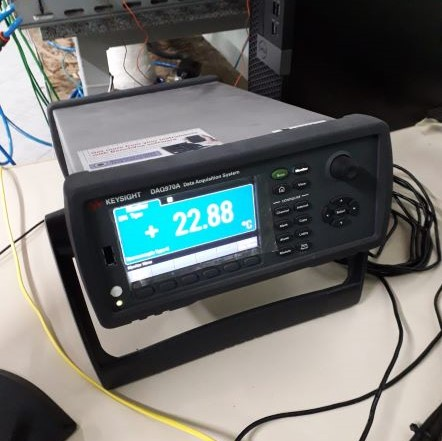
\includegraphics[scale=0.5]{Textuais/experimental/keysight.jpeg}}
	\frame{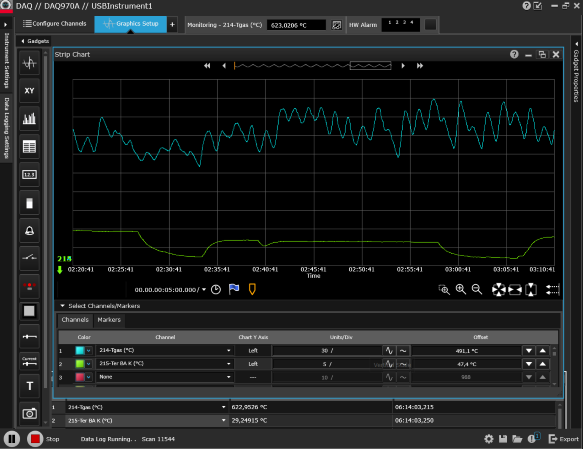
\includegraphics[scale=0.49]{Textuais/experimental/keysightbenchvue.png}}
	\fonte{O autor (2022).}
	\label{fig:keysight}
\end{figure}

O equipamento para medição de poluentes utilizado foi o Testo 350 (Figura \ref{fig:testo}), que conta com uma sonda que pode ser posicionada em cada um dos furos maiores da chaminé. O equipamento fornece dados de concentração de \ch{CO}, $\ch{NO}_x$, \ch{CO2}, \ch{O2} e hidrocarbonetos para um dado combustível, ajustado no equipamento previamente às medições. Todas as medições foram realizadas no topo da chaminé, posicionando-se a sonda no orifício logo acima ao perfil cônico.

\begin{figure}
	\centering
	\caption{Analisador de gases Testo 350.}
	\frame{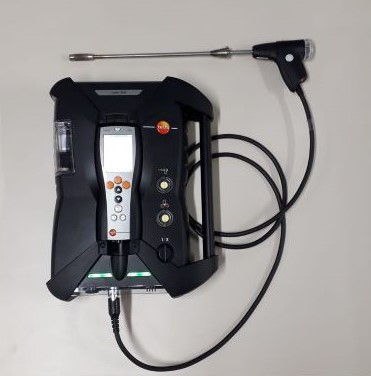
\includegraphics[scale=0.6]{Textuais/experimental/testo.jpeg}}
	\fonte{O autor (2022).}
	\label{fig:testo}
\end{figure}

\subsection{Vazão de combustível}
Os pellets de madeira são despejados no reator através de um sistema de alimentação, composto de um silo e um parafuso, acoplado a um motor elétrico trifásico. O motor é conectado a um controlador lógico programável (CLP), que permite ajustar os parâmetros relativos ao fornecimento de combustível. Esses parâmetros são:

\begin{enumerate}[noitemsep,nosep,labelindent=\parindent,leftmargin=*,label={\alph*})] 
	\item Tempo de descarga inicial: tempo em que a rosca despeja os pellets que serão usados na ignição do reator;
	\item Tempo de aguardo inicial: tempo entre a descarga de combustível inicial e o início do funcionamento do reator no modo automático;
	\item Tempo do ventilador: tempo para o qual o ventilador liga, a partir da descarga inicial;
	\item Tempo de descarga ($TH$): tempo no qual a rosca despeja pellets no reator, em modo automático;
	\item Tempo de aguardo ($TL$): intervalo de tempo entre as descargas de combustível, em modo automático.
\end{enumerate}

Os três primeiros parâmetros listados possuem função apenas no acendimento do reator, enquanto os dois últimos são fundamentais na análise do sistema operando em regime permanente. Nesse caso, é possível determinar a vazão mássica de combustível (Equação \eqref{eq:mdotpellet}) sabendo-se qual a massa de pellets despejada no tempo $TH$ ($m_{pellet} (TH)$) e o tempo de um ciclo ($T_{ciclo} = TL + TH$).
\begin{equation} \label{eq:mdotpellet}
\dot{m}_{comb} = \frac{m_{pellet} (TH)}{TL + TH}.
\end{equation}

O parâmetro $m_{pellet}(TH)$ médio foi determinado experimentalmente para diferentes tempos $TH$. O número de amostras $N$ necessário para a obtenção de uma média cujo desvio padrão populacional fosse $\sigma$, confiabilidade fosse $z$ e precisão fosse $L$, foi calculado com base na Equação \eqref{eq:ene}.
\begin{equation} \label{eq:ene}
N = \frac{z\sigma}{L}.
\end{equation}

O parâmetro $\sigma$ foi estimado a partir de 31 medições para $TL = 0,5$ s, número de medições para o qual pode-se usar o teorema do limite central \cite{Devore}. Para um parâmetro $z$ correspondente à 95\% de confiabilidade e precisão $L$ de 2 g, o número de amostras necessário foi $N=26$. A massa de pellets em cada amostra foi avaliada com uma balança de precisão Shimadzu, de resolução 0,01 g. A Tabela \ref{tab:mdot} relaciona os valores obtidos.

\begin{table}[!ht]
	\centering
	\small
	\renewcommand{\arraystretch}{1.3}
	\caption{Massa de combustível média fornecida ao reator para diferentes tempos de descarga.}%
	\label{tab:mdot}
        \begin{tabular}{|c|c|}
        \hline
        $TH$ (s) & $m_{pellet}(TH)$ (g)    \\ \hline
        0,1    & 10,87                     \\ \hline
        0,5    & 49,98                     \\ \hline
        1      & 96,22                     \\ \hline
        2      & 191,50                    \\ \hline
        \end{tabular}
    \vspace{2mm}
	\fonte{O autor (2022).}
\end{table}

\subsection{Vazão de ar}
%A vazão de ar é determinada usando-se um anemômetro de fio quente da fabricante Testo GmbH, modelo 445. Para uma melhor segurança em relação aos valores medidos, foi realizada uma aferição do equipamento em relação aos valores registrados, com o auxílio de uma câmara de teste de fluxo de ar da fabricante Airflow. A câmara conta com dois conjuntos de bocais, uma com 3 bocais de diâmetro externo 4 in e outra com 4 bocais, de diâmetros 2 in, 1,6 in, 1 in e 0,688 in. Um dos conjuntos é posicionado no centro da câmara e o outro na extremidade de saída. No momento em que o ar passa pelos bocais no centro do equipamento, existe uma queda na pressão do fluido, que é aferida com base em duas tomadas de pressão conectadas ao equipamento. Com a pressão manométrica sendo registrada por um manômetro de coluna de água Dwyer, e sendo conhecido o diâmetro dos bocais, é possível determinar a vazão de ar, através de cartas fornecidas pelo fabricante da câmara. Sabendo-se a vazão de ar e o diâmetro do bocal externo, é possível determinar a velocidade do ar teórica de maneira direta, tendo em vista que o bocal uniformiza o escoamento (i.e. a velocidade ao longo da seção transversal do bocal não varia), através da equação \eqref{eq:vazao}.
%\begin{equation} \label{eq:vazao}
%Q = V\cdot A.
%\end{equation}

%\noindent Essa velocidade, considerada como a teórica, é comparada com a velocidade registrada pelo anemômetro, que foi posicionado na saída do bocal. O procedimento foi realizado para 10 velocidades do ar, situadas no intervalo de 0 a 10 m/s. Para atingir essas velocidades, o bocal posicionado no centro do equipamento é o de 2 in, e na saída o de 4 in. A curva mostrada na Figura \ref{fig:curva} foi obtida.

%\begin{figure}
%	\centering
%	\caption{Curva de calibração obtida para o anemômetro.}
%	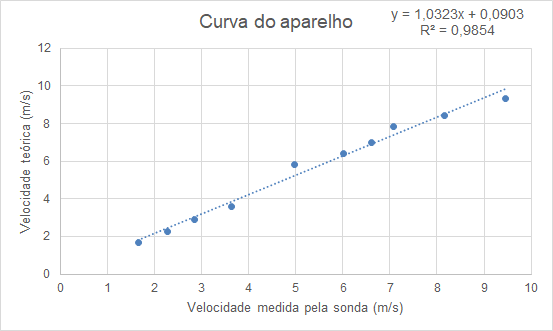
\includegraphics[scale=0.8]{Textuais/curva_calibracao_testo.png}
%	\fonte{O autor.}
%	\label{fig:curva}
%\end{figure}

O aparato experimental construído para medição da vazão consiste nos itens relacionados na lista abaixo. Uma visão geral do aparato experimental é mostrada na Figura \ref{fig:aparato}.
\begin{enumerate}[noitemsep,nosep,labelindent=\parindent,leftmargin=*,label={\alph*}) ] 
	\item Um bocal cônico para separação de fluxos de ar;
	\item Um tubo de PVC, de 75 mm de diâmetro nominal e 2,18 m de comprimento;
	\item Um tubo de Pitot, com ajuste de altura;
	\item Um manômetro de coluna de precisão da marca Dwyer.
\end{enumerate}

\begin{figure}[!ht]
	\centering
	\caption{Aparato experimental construído para medição da vazão.}
	\frame{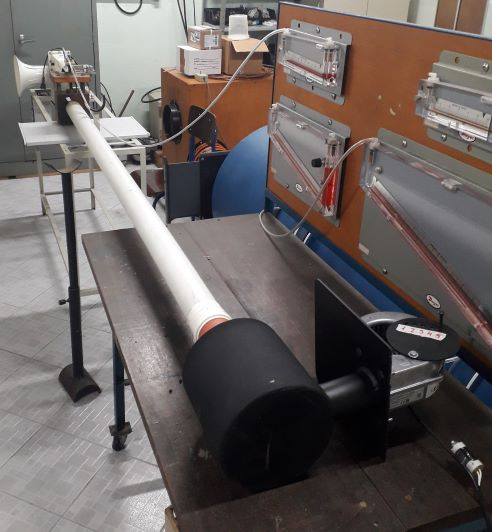
\includegraphics[scale=0.4]{Textuais/experimental/aparato.jpg}}
	\fonte{O autor (2022).}
	\label{fig:aparato}
\end{figure}

Vale ressaltar que as medições foram realizadas com o reator na horizontal, o que não influencia o resultado final. A medição da vazão de ar foi realizada em duas etapas: a primeira medição serviu para determinar somente a vazão da injeção primária, enquanto a segunda determinou a vazão total de ar (incluindo a injeção secundária). Para tanto foi usado o bocal cônico, como mostrado na Figura \ref{fig:cone}.

\begin{figure}[!ht]
	\centering
	\caption{Cone para separação dos fluxos de ar do fundo e das laterais.}
	\frame{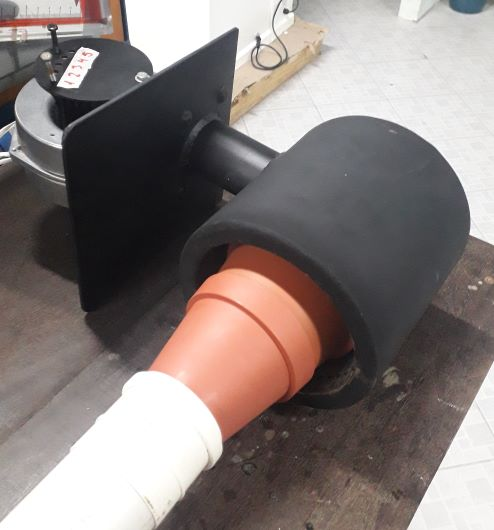
\includegraphics[scale=0.4]{Textuais/experimental/bottom.jpg}}
	\fonte{O autor (2022).}
	\label{fig:cone}
\end{figure}

O cone pode ser fixo em qualquer ponto ao longo da parede interna do reator. Portanto, para determinar a vazão proveniente do fundo do reator, o dispositivo foi fixado abaixo dos orifícios laterais, cuidando-se para que não haja obstrução desses (como é mostrado na Figura \ref{fig:cone}). Já para a medição da vazão total, o cone foi posicionado logo acima dos orifícios. Ao cone foi acoplado o tubo de PVC, que possui comprimento suficiente para permitir que o escoamento se torne completamente desenvolvido. O material do tubo possui rugosidade baixa, de forma que os efeitos de perda de carga não foram considerados.

A vazão de ar ar fornecida pelo ventilador acoplado ao queimador foi determinada considerando-se as 5 posições de ajuste da abertura de ar (Figura \ref{fig:posicoes}), convencionando-se a posição 1 para vazão máxima e a posição 5 para vazão mínima.

\begin{figure}[!ht]
	\centering
	\caption{Posições de abertura do ventilador.}
	\frame{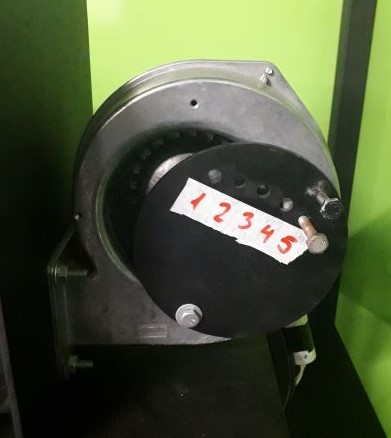
\includegraphics[scale=0.4]{Textuais/experimental/posicoes.jpg}}
	\fonte{O autor (2022).}
	\label{fig:posicoes}
\end{figure}

Para determinar a vazão de ar deve-se primeiramente obter a velocidade média do escoamento, que depende do regime desse (laminar ou turbulento). O regime de um escoamento interno em um tubo é avaliado pelo número de Reynolds relativo ao diâmetro, $Re_{D}$, Equação \eqref{eq:reynolds}.
\begin{equation} \label{eq:reynolds}
Re_D = \frac{VD}{\nu}.
\end{equation}

No caso de a quantia ser avaliada na posição de velocidade máxima do escoamento (linha central do tubo), $V = U$ e a notação é modificada para $Re_{U}$. Considerando a viscosidade cinemática do ar a 25°C na pressão atmosférica como $\nu = 1,5\cdot 10^{-5} m^2/s$ com base em dados de Fox (1998), espera-se um regime turbulento, de forma que não existe uma relação universal entre o campo de tensões e o campo de velocidade média \cite{Fox}. Uma das abordagens é usar um perfil experimental, sendo um dos mais usados o perfil de lei de potência, da forma da Equação \eqref{eq:perfil}.
\begin{equation} \label{eq:perfil}
\frac{\bar{u}}{U} = {\left(\frac{y}{R}\right)}^{1/n}.
\end{equation}

\noindent A coordenada $y$ possui origem na parede do tubo, sendo que para cada valor dessa coordenada é possível determinar uma velocidade média temporal $\bar{u}$ no ponto. O termo $n$ é determinado por correlações experimentais; Hinze apud Fox (1998) sugere que, para um escoamento interno em tubo liso, o expoente pode ser determinado pela Equação \eqref{eq:nturbulento}. 
\begin{equation} \label{eq:nturbulento}
n = -1,7 + 1,8\cdot log(Re_U).
\end{equation}

Na prática, o perfil previsto pela Equação \eqref{eq:perfil} pode ser avaliado com um tubo de Pitot, dispositivo com o qual é possível medir a variação da pressão de um escoamento em determinado ponto e então determinar a velocidade desse. O tubo de Pitot do aparato experimental conta com uma regulagem de altura, que permite medir a velocidade do escoamento ao longo do diâmetro do tubo. Um paquímetro também é acoplado, para permitir a medição do comprimento em relação à parede do tubo. A pressão obtida pelo tubo de Pitot é avaliada com base em um manômetro de coluna de água da fabricante Dwyer, com escala de 1 polegada de água ($in_{\ch{H2O}})$ e resolução de 0,01 $in_{\ch{H2O}}$. Ambos os dispositivos são mostrados na Figura \ref{fig:pitot}.

\begin{figure}[!ht]
	\centering
	\caption{Tubo de Pitot e manômetro de coluna de líquido.}
	\frame{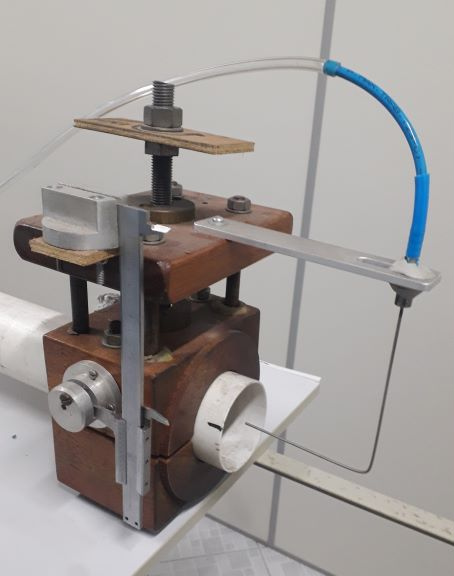
\includegraphics[scale=0.31]{Textuais/experimental/pitot_mini.jpg}}
	\frame{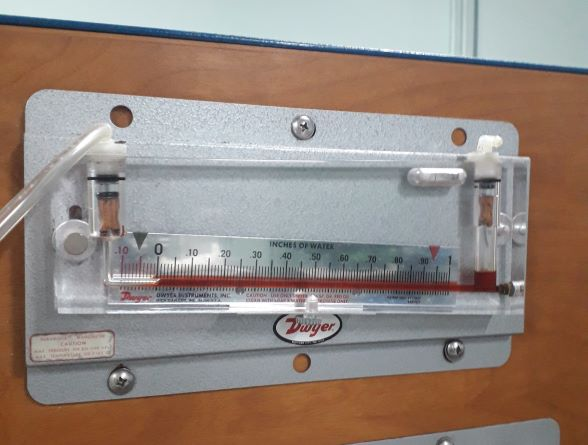
\includegraphics[scale=0.4]{Textuais/experimental/barometro.jpg}}
	\fonte{O autor (2022).}
	\label{fig:pitot}
\end{figure}

O tubo de Pitot fornece a pressão de estagnação $P_{0}$ do escoamento. Além dessa pressão, é necessário conhecer a pressão estática $P$. Como pode ser observado na Figura \ref{fig:pitot}, a ponta do tubo foi posicionada exatamente alinhada com o final do tubo de PVC, de forma que $P$ fio considerada a pressão atmosférica. Definindo a diferença de pressão como $\Delta P = P_{0} - P$, a velocidade do escoamento em qualquer posição ao longo do diâmetro do tubo pode ser determinada a partir da definição de pressão dinâmica, dando origem à Equação \eqref{eq:pitot}. O uso dessa expressão requer que o tubo esteja alinhado na horizontal, caso no qual a variação de energia potencial do escoamento pode ser desprezada. Dessa forma, o duto de PVC foi cuidadosamente alinhado na horizontal, com o auxílio de um nível.
\begin{equation} \label{eq:pitot}
V = \sqrt{\frac{2\Delta P}{\rho_{ar}}}.
\end{equation}

Assim, para verificar se o perfil de velocidade proposto por Hinze modela convenientemente o fenômeno, foi realizado um teste onde a pressão estática foi medida em vários pontos ao longo do diâmetro do tubo, visando a obtenção de um perfil de velocidade para uma vazão fixa. O valores de velocidade em função da posição obtidos são denotados pelos pontos azuis na Figura \ref{fig:vteoexp}, onde o sistema de coordenadas y possui origem na parede do tubo e termina na linha de centro. Com base no número de Reynolds da velocidade na linha de centro $Re_{U}$ foi determinado o expoente $n$ para essa velocidade, e com isso foi possível determinar um perfil de velocidade da forma da Equação \eqref{eq:perfil}, denotado pela linha vermelha na Figura \ref{fig:vteoexp}.

\begin{figure}[!ht]
	\centering
	\caption{Pontos experimentais e perfil de velocidade previsto pela Equação \eqref{eq:perfil}}.
	\frame{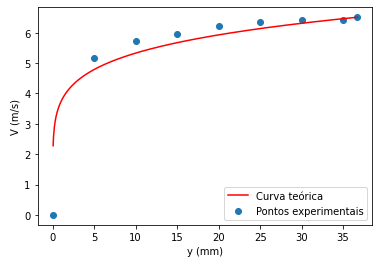
\includegraphics[scale=0.8]{Textuais/experimental/vteoexp.png}}
	\fonte{O autor (2022).}
	\label{fig:vteoexp}
\end{figure}

Como observado pelo gráfico, a curva traçada com base na Equação \eqref{eq:perfil} apresentou-se próxima às velocidades experimentais obtidas para cada ponto, sendo que o erro máximo verificado entre os pontos experimentais foi de 7,67\%, em y = 10 mm. Destaca-se que o perfil teórico não descreve bem o comportamento próximo à parede (para valores de $y/R < 0,04$), e não possui inclinação nula no centro, fato que pode ser observado no gráfico; todavia, são erros inerentes ao modelo \cite{Fox}. Devido à simplicidade matemática e boa aproximação do comportamento real, o modelo de perfil de potência será usado, permitindo o uso das Equações \eqref{eq:nturbulento} e \eqref{eq:vsobreu}. 

Para determinar a vazão volumétrica, é necessário determinar a velocidade média do escoamento ($\bar{V}$), a qual pode ser estimada com base na medição experimental da velocidade apenas na linha de centro ($U$) e no expoente $n$, conforme apresentado pela Equação \eqref{eq:vsobreu}, obtida por meio da integração da Equação \eqref{eq:perfil}.
\begin{equation} \label{eq:vsobreu}
\frac{\bar{V}}{U} = \frac{2n^{2}}{(n+1)(2n+1)}.
\end{equation}

\noindent Sendo conhecida $\bar{V}$, a vazão volumétrica pode ser determinada pela Equação \eqref{eq:vazaovol}.
\begin{equation} \label{eq:vazaovol}
{Q} = {\bar{V}} \cdot A_{tr}.
\end{equation}
\noindent O termo $A_{tr}$ representa a área da seção transversal do tubo, cujo diâmetro é de 70
mm. Dessa forma, o procedimento experimental consistiu nas seguintes etapas:




\begin{enumerate}[noitemsep,nosep,labelindent=\parindent,leftmargin=*,label={\alph*}) ] 
	\item Medição da velocidade no centro do tubo utilizando-se o tubo de Pitot;
	\item Determinação da velocidade média do escoamento ($\bar{V}$) por meio da Equação \eqref{eq:vsobreu};
	\item Determinação da vazão volumétrica ($Q$).
\end{enumerate}

A partir dos procedimentos descritos, as vazões volumétricas foram medidas e estão apresentadas na Tabela \ref{tab:vazoes}, sendo os valores apresentados em $m^3/s$ e litros por minuto (LPM).

\begin{table}[!ht]
	\centering
	\small
	\renewcommand{\arraystretch}{1.3}
	\caption{Vazões volumétricas obtidas para as 5 posições de abertura do ventilador.}%
	\label{tab:vazoes}
        \begin{tabular}{|c|cc|cc|cc|}
        \hline
        \multirow{2}{*}{Posição} & \multicolumn{2}{c|}{Injeção primária} & \multicolumn{2}{c|}{Total}            & \multicolumn{2}{c|}{Injeção secundária} \\ \cline{2-7} 
                         & \multicolumn{1}{c|}{m³/s}    & LPM    & \multicolumn{1}{c|}{m³/s}    & LPM    & \multicolumn{1}{c|}{m³/s}      & LPM    \\ \hline
        1                        & \multicolumn{1}{c|}{0,0222}  & 1332,0 & \multicolumn{1}{c|}{0,03517} & 2110,2 & \multicolumn{1}{c|}{0,01292}   & 775,2  \\ \hline
        2                        & \multicolumn{1}{c|}{0,0221}  & 1326,0 & \multicolumn{1}{c|}{0,03466} & 2079,6 & \multicolumn{1}{c|}{0,01253}   & 751,8  \\ \hline
        3                        & \multicolumn{1}{c|}{0,0219}  & 1314,0 & \multicolumn{1}{c|}{0,03356} & 2013,6 & \multicolumn{1}{c|}{0,01165}   & 699,0  \\ \hline
        4                        & \multicolumn{1}{c|}{0,0210}  & 1260,0 & \multicolumn{1}{c|}{0,03281} & 1968,6 & \multicolumn{1}{c|}{0,01181}   & 708,6  \\ \hline
        5                        & \multicolumn{1}{c|}{0,0193}  & 1158,0 & \multicolumn{1}{c|}{0,03044} & 1826,4 & \multicolumn{1}{c|}{0,01114}   & 668,4  \\ \hline
        \end{tabular}
	\vspace{2mm}
	\fonte{O autor.}
\end{table}

Pode-se observar que a posição de abertura da placa posicionada na entrada no ventilador resultou na variação da vazão de ar total em torno de 13\%. Ainda, a vazão na injeção secundária representa cerca de 36\% da vazão total para todas as posições de abertura do ventilador.

Um teste preliminar do queimador em operação foi realizado a fim de determinar se as vazões de ar obtidas permitem um funcionamento adequado do queimador. Para uma injeção de combustível de 1 s a cada 40 s, para a menor vazão de ar (posição 5), verificou-se uma chama muito intensa, como pode ser verificado na Figura \ref{fig:preliminar}. Essa chama inviabilizaria as medições, principalmente da emissão de poluentes.

\begin{figure}[!ht]
	\centering
	\caption{Teste preliminar do queimador com a vazão de ar de 1826,4 LPM (posição 5).}
	\frame{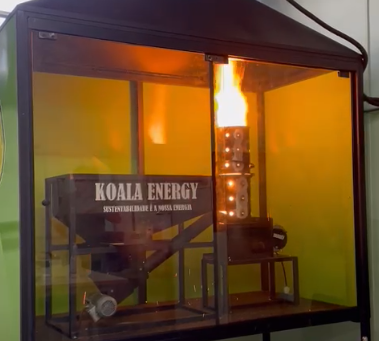
\includegraphics[scale=0.8]{Textuais/experimental/preliminar.png}}
	\fonte{O autor (2022).}
	\label{fig:preliminar}
\end{figure}

Assim, buscou-se por um mecanismo que pudesse diminuir a vazão volumétrica de ar. Optou-se por uma placa de orifícios, que permite reduzir o fluxo de ar sem a necessidade de ajustar características elétricas do ventilador. Além disso, foram feitos mais dois orifícios na placa de controle de vazão, permitindo o ajuste de mais duas posições da placa, que permite mais dois valores de vazão (inferores aos já existentes). Esses orifícios foram nomeados 6 e 7, respectivamente. Para registrar as novas vazões volumétricas o procedimento adotado, bem como as equações utilizadas, foram idênticos ao caso anterior. Entretanto, as pressões registradas através do tubo de Pitot eram muito baixas, de forma que para uma medição mais precisa de velocidade foi usado um anemômetro de fio quente, da fabricante Testo GmbH, modelo 445. O anemômetro foi posicionado na extremidade do tubo, no centro desse em relação à seção transversal, na posição onde anteriormente estava o tubo de Pitot, como mostra a Figura \ref{fig:fioquente}. As novas vazões obtidas são mostradas na Tabela \ref{tab:vazoesnova}.

\begin{figure}[!ht]
	\centering
	\caption{Posicionamento do anemômetro de fio quente.}
	\frame{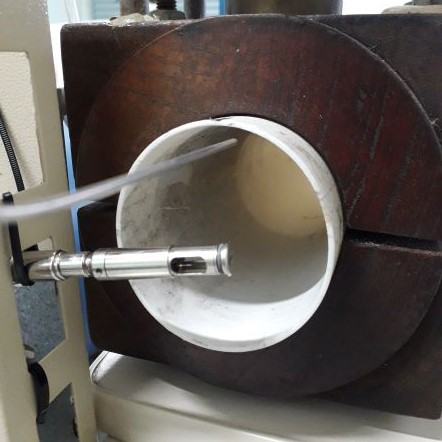
\includegraphics[scale=0.4]{Textuais/experimental/fiquente.jpg}}
	\fonte{O autor (2022).}
	\label{fig:fioquente}
\end{figure}


\begin{table}[!htbp]
	\centering
	\small
	\renewcommand{\arraystretch}{1.3}
	\caption{Novas vazões volumétricas medidas.}%
	\label{tab:vazoesnova}
        \begin{tabular}{|c|cc|cc|cc|}
        \hline
        \multirow{2}{*}{Posição} & \multicolumn{2}{c|}{Injeção primária} & \multicolumn{2}{c|}{Total}           & \multicolumn{2}{c|}{Injeção secundária} \\ \cline{2-7} 
                                 & \multicolumn{1}{c|}{m³/s}     & LPM   & \multicolumn{1}{c|}{m³/s}    & LPM   & \multicolumn{1}{c|}{m³/s}      & LPM    \\ \hline
        1                        & \multicolumn{1}{c|}{0,00239}  & 143,4 & \multicolumn{1}{c|}{0,00478} & 286,5 & \multicolumn{1}{c|}{0,00239}   & 143,2  \\ \hline
        2                        & \multicolumn{1}{c|}{0,00232}  & 139,4 & \multicolumn{1}{c|}{0,00461} & 276,4 & \multicolumn{1}{c|}{0,00228}   & 137,0  \\ \hline
        3                        & \multicolumn{1}{c|}{0,00226}  & 135,4 & \multicolumn{1}{c|}{0,00454} & 272,3 & \multicolumn{1}{c|}{0,00228}   & 136,9  \\ \hline
        4                        & \multicolumn{1}{c|}{0,00222}  & 133,4 & \multicolumn{1}{c|}{0,00437} & 262,2 & \multicolumn{1}{c|}{0,00215}   & 128,7  \\ \hline
        5                        & \multicolumn{1}{c|}{0,00209}  & 125,5 & \multicolumn{1}{c|}{0,00420} & 252,0 & \multicolumn{1}{c|}{0,00211}   & 126,6  \\ \hline
        6                        & \multicolumn{1}{c|}{0,00196}  & 117,5 & \multicolumn{1}{c|}{0,00403} & 241,9 & \multicolumn{1}{c|}{0,00207}   & 124,4  \\ \hline
        7                        & \multicolumn{1}{c|}{0,00179}  & 107,6 & \multicolumn{1}{c|}{0,00383} & 229,8 & \multicolumn{1}{c|}{0,00204}   & 122,1  \\ \hline
        \end{tabular}
	\vspace{2mm}
	\fonte{O autor (2022).}
\end{table}

Verifica-se que a proporção de 36\% estimada pelos testes iniciais não se manteve, sendo alterada para valores próximos de 50\%. Ou seja, a quantidade de ar destinada aos processos de volatilização e oxidação é aproximadamente igual.


\section{Parâmetros de operação como função das variáveis medidas}
Para determinar os parâmetros de operação do queimador de acordo com os parâmetros iniciais, foi elaborado um código computacional no software EES (Engineering Equation Solver). A fim de determinar uma expressão para a razão de equivalência ($\Phi$), é necessário inicialmente conhecer a fração combustível-ar estequiométrica ($F_s$), obtida pela equação química da reação global que ocorre com o pellet. Tendo em vista que os pellets possuem um teor de enxofre usualmente desprezível, a Equação química \eqref{eq:combestbio} se reduz a Equação \eqref{eq:combpellet}.
\begin{equation} \label{eq:combpellet}
\ch{C} \ch{H}_a \ch{O}_b \ch{N}_c + a_t(\ch{O2} + 3,76 \ch{N2}) \rightarrow{} x \ch{CO2} + y \ch{H2O} + w \ch{N2}.
\end{equation}

\noindent A reação pode ser reescrita em base molar, sendo cada componente do combustível especificado separadamente. 
\begin{equation} \label{eq:combpelletn}
n_c \ch{C} + n_H \ch{H} + n_O \ch{O} + n_N \ch{N} + a_t(\ch{O2} + 3,76 \ch{N2}) \rightarrow{} x \ch{CO2} + y \ch{H2O} + w \ch{N2}.
\end{equation}

\noindent Na Equação \eqref{eq:combpelletn} $n_i$ é definido como segue. $MW_i$ é a massa molar de cada componente, e as frações $Y_i$ são obtidas da Tabela \ref{tab:elementar_modelagem}.
\begin{equation} \label{eq:enee}
n_i = \frac{Y_i}{MW_i}.
\end{equation}
% em kmol/kgcomb

Aplicando-se a conservação da massa para cada espécie química:
\begin{enumerate}[noitemsep,nosep,labelindent=\parindent,leftmargin=*,label={\alph*}) ] 
	\item Balanço de \ch{C}:
	\begin{equation}
	    x = n_C.    
	\end{equation}
	\item Balanço de \ch{H}:
	\begin{equation}
	    n_H = 2y.    
	\end{equation}
    \item Balanço de \ch{O}:
	\begin{equation}
	    n_O + a_t = 2x + y.    
	\end{equation}
    \item Balanço de \ch{N}:
	\begin{equation}
	    a_t\cdot3,76\cdot2 = 2w.    
	\end{equation}
\end{enumerate}

\noindent O termo $F_s$, considerando-se a combustão completa de 1 kg de combustível, é dada pela Equação \eqref{eq:Fs}. A massa molecular do ar foi determinada a 25°C e 1 atm diretamente através do EES.
\begin{equation} \label{eq:Fs}
F_s = \frac{n_C\cdot MW_C + n_H\cdot MW_H + n_O\cdot MW_O + n_N\cdot MW_N}{4,76\cdot a_t \cdot MW_{ar}}.
\end{equation}

\noindent Em termos dos dados fornecidos, a fração combustível-ar $F$ é dada por:
\begin{equation} \label{eq:F}
F = \frac{\dot{m}_{comb}}{\dot{m}_{ar}}
\end{equation}

\noindent onde o termo $\dot{m}_{comb}$ é dado pela Equação \eqref{eq:mdotpellet} e $\dot{m}_{ar}$ provém da Tabela \ref{tab:vazoesnova}, bastando-se apenas converter os valores de vazão total de $m^3/s$ para $kg/s$ através da densidade do ar $\rho_{ar}$, avaliada a 25°C e 1 atm.
\begin{equation} \label{eq:VtoM}
\dot{m}_{ar} \left[\frac{kg}{s}\right]= {Q}_{ar} \left[\frac{m^3}{s}\right] \cdot \rho_{ar} \left[\frac{kg}{m^3}\right]
\end{equation}

As Equações \eqref{eq:VtoM}, \eqref{eq:F}, \eqref{eq:Fs}, \eqref{eq:mdotpellet}, \eqref{eq:Pot} e \eqref{eq:phi} foram reunidas no código computacional. Para determinar os parâmetros de operação do queimador, é necessário somente informar três variáveis iniciais; para os testes realizados, foram informados os valores da vazão volumétrica de ar total ${Q}_{ar}$, razão de equivalência $\Phi$ desejada e tempo de despejo $TH$. O EES permite a construção de tabelas paramétricas, de forma que os dados foram arranjados nesse modelo, como mostrado pela Figura \ref{fig:tabparam}. 

\begin{figure}[!ht]
	\centering
	\caption{Exemplo de tabela paramétrica do EES.}
	\frame{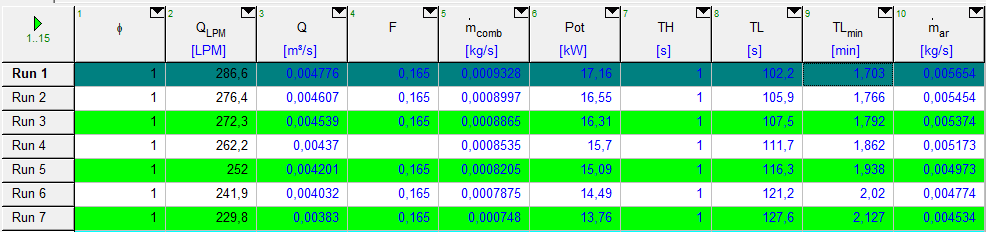
\includegraphics[scale=0.6]{Textuais/experimental/tabela_EES.png}}
	\fonte{O autor (2022).}
	\label{fig:tabparam}
\end{figure}

\section{Execução dos testes}
Os testes consistiram em avaliações quantitativas e qualitativas do processo de combustão no reator, com o sistema operando em regime automático (com alimentações de combustível periódicas). O primeiro teste consistiu na verificação do comportamento da chama e das condições de operação do reator para $\Phi = 1$ em 4 potências, avaliando de maneira visual a intensidade da chama e a estabilização das reações ao longo do tempo. Da mesma forma, o segundo conjunto de testes consistiu na mesma avaliação para $\Phi = 0,7$, dessa vez para 3 potências. As imagens para determinar o perfil da chama foram registradas a uma distância padronizada do queimador. Os testes qualitativos permitiram uma validação preliminar do aparato experimental, permitindo ajustes importantes antes do início das medições. A partir dos primeiros testes também foi possível determinar os melhores parâmetros para acendimento do reator, sendo eles:

\begin{enumerate}[noitemsep,nosep,labelindent=\parindent,leftmargin=*,label={\alph*})] 
	\item Tempo de descarga inicial: 5 segundos;
	\item Tempo de aguardo inicial: 7 minutos;
	\item Tempo do ventilador: 4 minutos (após o tempo de descarga inicial);
\end{enumerate}

O terceiro conjunto de testes consistiu propriamente na medição de temperatura e emissão de poluentes do queimador. Nesses testes foi usada a chaminé, já devidamente isolada, sendo um teste realizado para $\Phi = 1$ e três testes para $\Phi = 0,7$. O perfil de temperatura obtido para todos os testes foi oscilatório, como já esperado inicialmente, tendo em vista o fato da alimentação ser intermitente. Dessa forma, para determinar se o sistema estava em regime permanente, foi verificada a amplitude do perfil de temperatura; se esse intervalo se mostrava dentro de uma mesma faixa de temperatura por aproximadamente 20 minutos, o processo era considerado em regime permanente. Após a estabilização, foram realizadas as medições de emissão de poluentes, sendo a sonda posicionada no orifício de medição superior da chaminé por aproximadamente 7 minutos, sendo 2 minutos necessários para estabilização dessas medições. O processo é mostrado na Figura \ref{fig:eu}.

\begin{figure}[!t]
	\centering
	\caption{Medição de poluentes sendo realizada.}
	\frame{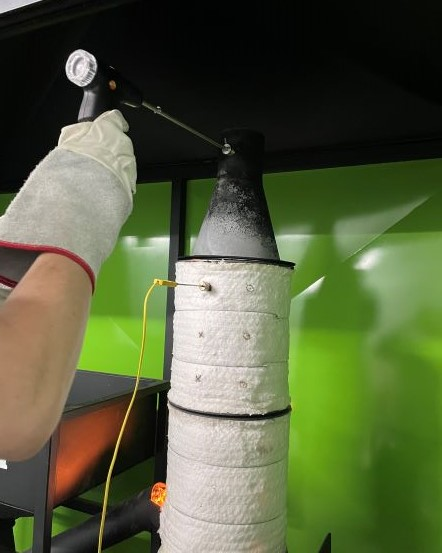
\includegraphics[scale=0.5]{Textuais/results/medindo.jpeg}}
	\fonte{O autor (2022).}
	\label{fig:eu}
\end{figure}


% \section{Infos adicionais}
% Medidas experimentais do diâmetro do queimador:

% $d_1 = 20,35 cm$

% $d_2 = 20,3 cm$

% $d_3 = 20,28 cm$

% $d_4 = 20,38 cm$

% $d_5 = 20,3 cm$

% Vídeos de queimadores semelhantes:

% https://www.youtube.com/watch?v=kvRK0lC1UKk

% https://www.youtube.com/watch?v=5Oxm-sO39MM

% https://www.youtube.com/watch?v=4OqJTvxrdLw

% Testes que podem ser realizados:

% - Fixar vazão mássica e ver o comportamento em 5 vazões de ar distintas (estimar phi para cada caso)

% - Determinar a potência máxima 

% - Emissão de poluentes (provavelmente somente para a menor vazão, pra não danificar o testo): CO, NOx, CO2

% - Distribuição de temperaturas (se possível)

% Coisas pra fazer

% - Fotos sem o tubo de Pitot


\chapter{Resultados e discussões}

\section{Aspecto da chama em regime permanente}

\subsection{Razão de equivalência 1}
O objetivo inicial foi avaliar o comportamento do reator de maneira qualitativa, variando-se a vazão volumétrica de ar para uma razão de equivalência constante. Os parâmetros de teste usados nos testes são mostrados na Tabela \ref{tab:phi1}.

\begin{table}[!htbp]
	\centering
	\small
	\renewcommand{\arraystretch}{1.3}
	\caption{Parâmetros do ensaio.}%
	\label{tab:phi1}
        \begin{tabular}{|l|c|c|c|c|}
        \hline
        \textbf{Posição do ventilador} & \multicolumn{1}{c|}{\textbf{7}} & \textbf{5}              & \textbf{3} & \textbf{1} \\ \hline
        ${Q}_{ar}$ (LPM)           & 229,8                           & 252,0                   & 272,3      & 286,6      \\ \hline
        $\Phi$                         & 1                               & 1                       & 1          & 1          \\ \hline
        $\dot{m}_{comb}$ ($g/s$)       & 0,748                           & 0,8205                  & 0,8865     & 0,9328     \\ \hline
        P (kW)                         & 13,76                           & 15,09                   & 16,31      & 17,16      \\ \hline
        TH (s)                         & 1                               & 1                       & 1          & 1          \\ \hline
        TL (s)                         & 127                             & 116                     & 107        & 102        \\ \hline
        $T_{admin, ar}$ (°C)           & 32                              & 31 & 31         & 31         \\ \hline
        \end{tabular}
    \vspace{2mm}
	\fonte{O autor.}
\end{table}

Para $\Phi = 1$, em 4 potências diferentes, o aspecto da chama é mostrado na Figura \ref{fig:4chamasphi1}. Em (a) a potência é a maior de todas, enquanto em (d) é a menor. Percebe-se que a altura da chama diminui conforme aumenta a potência. Esse fenômeno possivelmente decorre da geometria do queimador. Quanto maior a potência, mais ar é injetado no queimador, aumentando a vazão secundária de ar. Quando a vazão secundária aumenta, a chama é direcionada ao centro do reator, havendo inclusive a formação de vórtices, como mostrado na Figura \ref{fig:chamas}.

\begin{figure}[!ht]
    \centering
	\caption{Aspecto da chama para as 4 diferentes potências testadas.}
	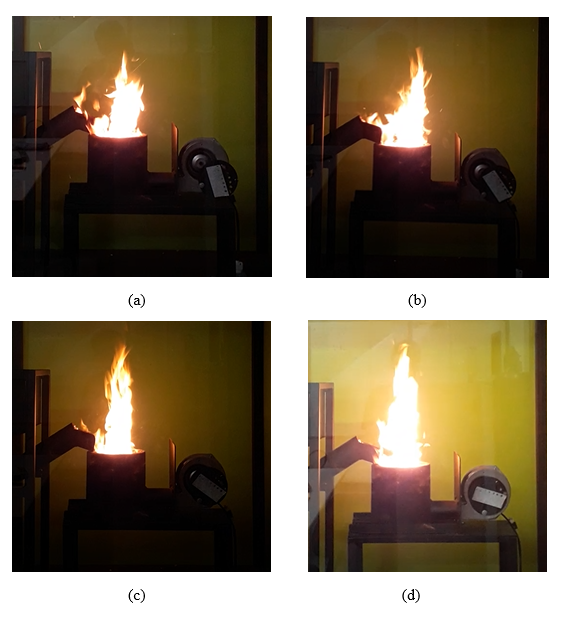
\includegraphics[scale=1]{Textuais/results/4chamas.png}
	\fonte{O autor (2022).}
	\label{fig:4chamasphi1}
\end{figure}

\begin{figure}[!ht]
	\centering
	\caption{Comparação entre a chama de menor potência (esquerda) e maior potência (direita).}
	\frame{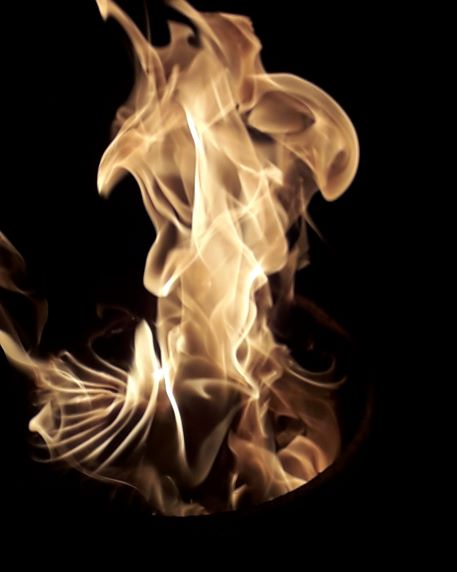
\includegraphics[scale=0.4]{Textuais/results/phi1pos7.jpg}}
	\frame{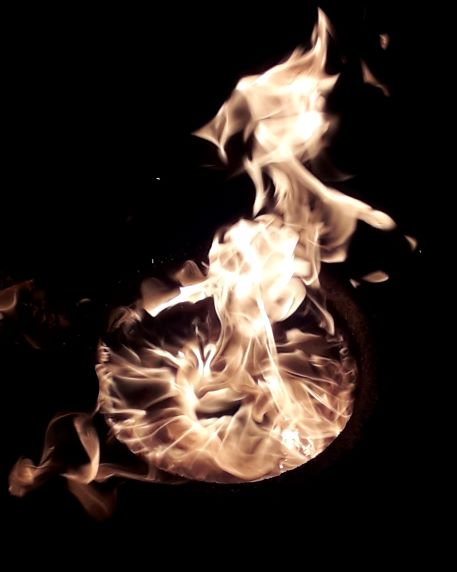
\includegraphics[scale=0.4]{Textuais/results/phi1pos1.jpg}}
	\fonte{O autor (2022).}
	\label{fig:chamas}
\end{figure}

Outro aspecto relevante na análise da chama é a distribuição dos pellets dentro do queimador. Na disposição em que o alimentador foi posicionado, o combustível tende a ficar acumulado do lado direito do queimador. Essa distribuição em alguns momentos tornou a chama assimétrica, principalmente para uma potência baixa, como verificado na Figura \ref{fig:assimetria} (potência 7).

\begin{figure}
	\centering
	\caption{Assimetria da chama.}
	\frame{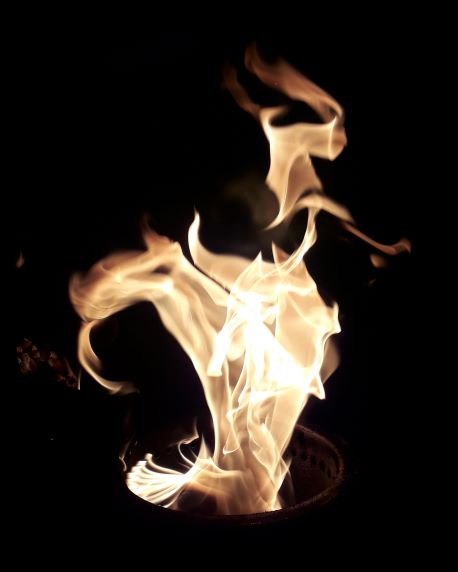
\includegraphics[scale=0.4]{Textuais/results/assimetria.jpg}}
	\fonte{O autor.}
	\label{fig:assimetria}
\end{figure}

\noindent Na Figura \ref{fig:assimetria} percebe-se que a injeção de ar secundária influencia mais a chama do lado da alimentação, em relação ao lado oposto. Isso se deve pois, tendo em vista que a vazão mássica é baixa, não há vazão suficiente de pellets para preencher a superfície da grade, fazendo com que o combustível se concentre no lado do alimentador.

Nesse ensaio, para cada potência considerou-se o tempo de estabilidade como sendo aproximadamente 40 minutos. Nesse intervalo, para todas as potências a chama se sustentou de maneira satisfatória. Entretanto, na potência mais alta foi constatado que o nível de pellets no queimador subiu ao longo do tempo. O equipamento foi mantido em regime automático por um tempo adicional de 20 minutos, a fim de verificar se o fenômeno persistiria. Ao final desse tempo, observou-se que o nível de pellets dentro do reator alcançava a injeção secundária de ar (Figura \ref{fig:transb}), o que certamente resultaria na extinção da chama. 

\begin{figure}[!ht]
	\centering
	\caption{Nível de pellets excessivo, alcançando o topo do reator.}
	\frame{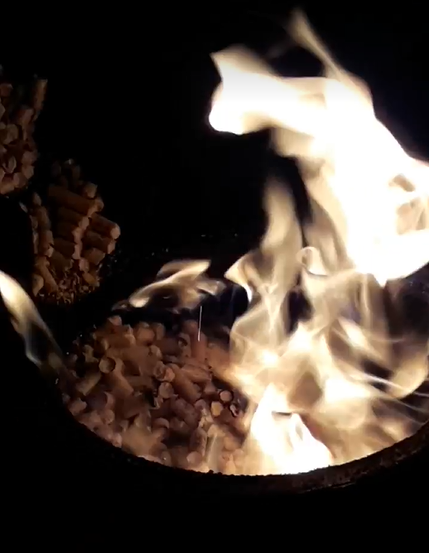
\includegraphics[scale=0.5]{Textuais/results/transbordando.png}}
	\fonte{O autor (2022).}
	\label{fig:transb}
\end{figure}

Esse transbordamento indica que a volatilização de uma certa quantidade de combustível não ocorre em tempo hábil antes de uma próxima carga ser inserida. Esse resultado aponta para a necessidade uma análise aprofundada da cinética química que rege as equações de volatilização e queima nesse reator, o que foge ao escopo do presente trabalho. Portanto, o ponto de potência 1 (maior potência) foi considerado como instável. 
\subsection{Razão de equivalência 0,7}
Para a razão de equivalência $\Phi = 0,7$ foram avaliadas três potências de operação, tendo em vista que no terceiro ensaio foi verificada uma leve tendência de o nível de pellets subir, sendo possível inferir que para a maior potência esse aumento de nível ocorreria de maneira semelhante ao que ocorreu para $\Phi=1$. Os parâmetros usados são mostrados na Tabela \ref{tab:phi0,7}.

\begin{table}[!ht]
	\centering
	\small
	\renewcommand{\arraystretch}{1.3}
	\caption{Parâmetros do ensaio.}%
	\label{tab:phi0,7}
        \begin{tabular}{|l|c|c|c|}
        \hline
        \textbf{Posição do ventilador} & \textbf{7} & \textbf{5} & \textbf{3} \\ \hline
        ${Q}_{ar}$ (LPM)           & 229,8      & 252,0      & 272,3      \\ \hline
        $\Phi$                         & 0,7        & 0,7        & 0,7        \\ \hline
        $\dot{m}_{comb}$ ($g/s$)       & 0,5236     & 0,5743     & 0,6206     \\ \hline
        P (kW)                         & 9,63       & 10,57      & 11,42      \\ \hline
        TH (s)                         & 1          & 1          & 0,5          \\ \hline
        TL (s)                         & 182        & 166           & 80          \\ \hline
        $T_{admin, ar}$ (°C)           & 29         & 28         & 29         \\ \hline
        \end{tabular}
    \vspace{2mm}
	\fonte{O autor (2022).}
\end{table}

O aspecto da chama para os três testes é mostrado na Figura \ref{fig:phi0,7tres}. Buscou-se capturar as imagens no momento em que a chama estabiliza, o que acontece aproximadamente na metade do tempo $TL$. Tal como na análise para $\Phi = 1$, de maneira geral a chama tende a ser mais alta para potências mais baixas, pelos mesmos motivos já comentados para aqueles resultados. 

\begin{figure}[!ht]
     \centering
        \caption{Aspecto da chama nos três diferentes testes.}
        \label{fig:phi0,7tres}
     \begin{subfigure}[b]{0.3\textwidth}
         \centering
         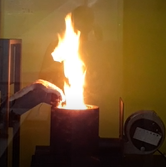
\includegraphics[width=\textwidth]{Textuais/results/0,7posicao7.png}
         \caption{Potência 7}
         \label{fig:pot7}
     \end{subfigure}
     \hfill
     \begin{subfigure}[b]{0.3\textwidth}
         \centering
         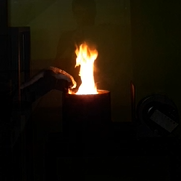
\includegraphics[width=\textwidth]{Textuais/results/0,7posicao5.png}
         \caption{Potência 5}
         \label{fig:pot5}
     \end{subfigure}
     \hfill
     \begin{subfigure}[b]{0.3\textwidth}
         \centering
         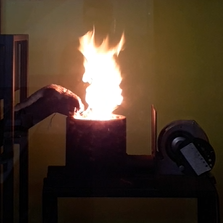
\includegraphics[width=\textwidth]{Textuais/results/0,7posicao3.png}
         \caption{Potência 3}
         \label{fig:pot3}
     \end{subfigure}
     \fonte{O autor (2022).}
\end{figure}

Uma particularidade dessa razão de equivalência é que o intervalo $TL$ se torna bastante longo, fazendo com que as propriedades da combustão variem consideravelmente nesse intervalo, o que se reflete no aspecto da chama. A sequência de imagens mostradas na Figura \ref{fig:perfilchama3_0,7} mostra a variação da chama ao longo do tempo, dentro de um intervalo $TL$, para a potência de 11,42 kW (posição 3 do ventilador). A primeira imagem foi capturada logo após a primeira alimentação, e as demais em intervalos periódicos de 15 segundos. Nessas condições, espera-se que as propriedades relativas à combustão (principalmente temperatura e emissões) variem mais a cada ciclo.  

\begin{figure}[!ht]
	\centering
	\caption{Perfil da chama em um mesmo intervalo $TL$.}
	\frame{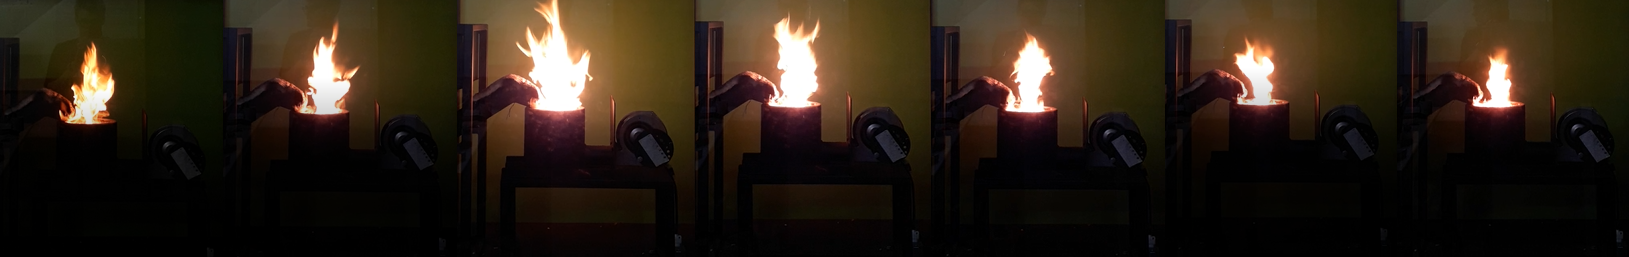
\includegraphics[scale=0.35]{Textuais/results/perfil_chama_0,7_3.png}}
	\fonte{O autor (2022).}
	\label{fig:perfilchama3_0,7}
\end{figure}

Em se tratando de combustão com mistura pobre ($\Phi < 1$), inicialmente esperava-se uma chama de coloração mais azulada. Todavia, como a massa de combustível no reator varia periodicamente, e a mistura acaba sendo bastante heterogênea, essa característica não foi observada. Somente ao final do experimento, quando o alimentador foi desligado e a massa de combustível contida no queimador espalhada uniformemente na grelha, foi possível observar essa chama de aspecto azulado (Figura \ref{fig:chamaazul}).

\begin{figure}[!ht]
	\centering
	\caption{Chama típica de misturas pobres, obtida no fim dos experimentos.}
	\frame{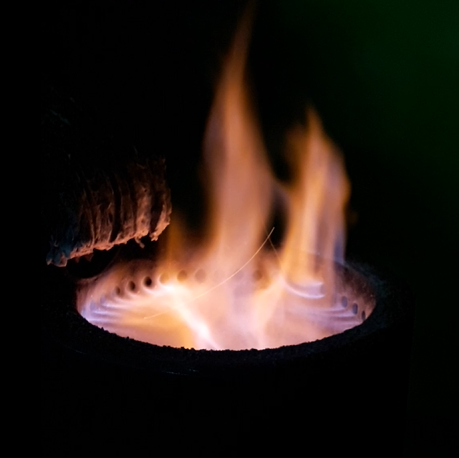
\includegraphics[scale=0.52]{Textuais/results/chama_azul.png}}
	\frame{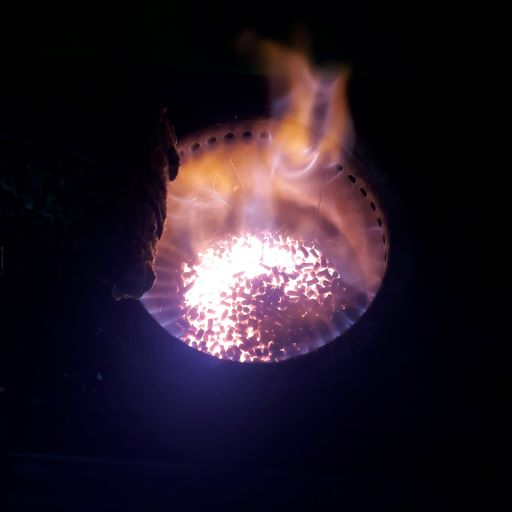
\includegraphics[scale=0.35]{Textuais/results/chama_azul_fundo.jpg}}
	\fonte{O autor (2022).}
	\label{fig:chamaazul}
\end{figure}

%%%%%%%%%%%%%%%%%%%%%%%%%%%%%%%%%%%%%%%%%%%%%%%%%%%%%%%%%%%%%%%%%%%%%%%%%%%%%%%%%%%%%%%%%%%%%%%%%%%%%%%%%%%%%%%%%%%%
\section{Temperatura e emissão de poluentes}

\subsection{Razão de equivalência 1}
Inicialmente buscou-se trabalhar com $\Phi = 1$, com a menor potência disponível (usando os parâmetros da segunda coluna da Tabela \ref{tab:phi1}). Entretanto, tendo em vista que a chaminé possui isolamento térmico, as temperaturas se elevaram, o que proporcionou a formação de uma chama muito alta (na Figura \ref{fig:demais} verifica-se que a chama termina no topo da chaminé). Essa chama, além de reduzir a vida útil do termopar, pode danificar a sonda de medição de gases. Para viabilizar as medições, optou-se então por trabalhar com $\Phi = 0,7$.

\begin{figure}[!ht]
	\centering
	\caption{Tentativa de medição para $\Phi = 1$, P = 13,76 kW.}
	\frame{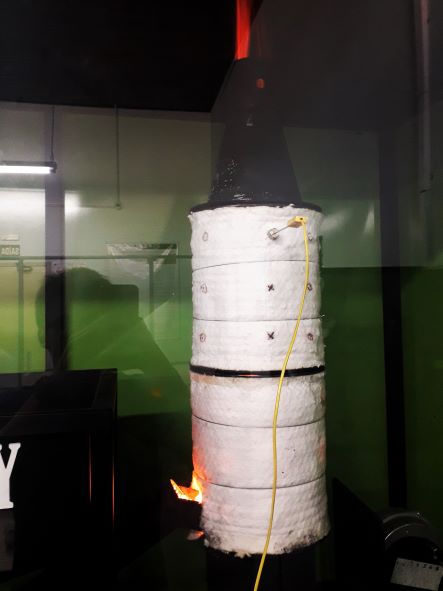
\includegraphics[scale=0.4]{Textuais/results/phi1poluentes.jpg}}
	\fonte{O autor (2022).}
	\label{fig:demais}
\end{figure}

\subsection{Razão de equivalência 0,7}
Os ensaios para $\Phi = 0,7$ foram realizados com base nos dados da Tabela \ref{tab:phi0,7}. Para cada caso, esperou-se a estabilização da temperatura dos gases dentro de um intervalo relativamente fixo. A  Figura \ref{fig:est_temp} mostra as temperaturas registradas dentro da faixa de estabilidade, sendo as linhas tracejadas a média para cada potência.

\begin{figure}[!ht]
	\centering
	\caption{Temperaturas registradas na estabilidade, para cada potência.}
	\frame{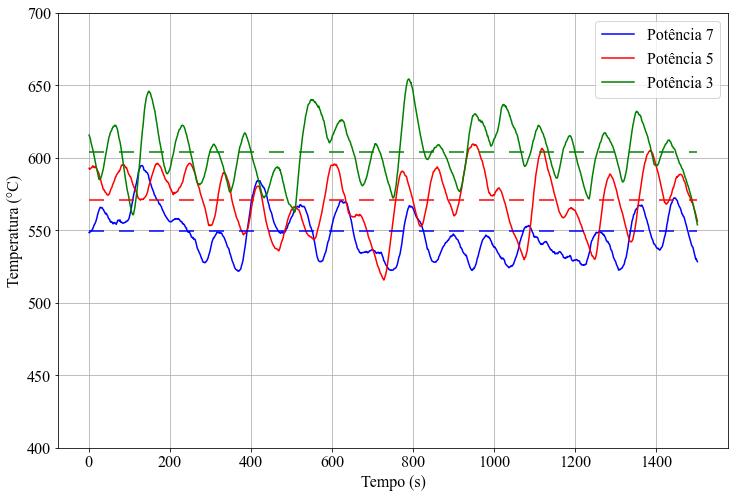
\includegraphics[scale=0.4]{Textuais/results/estabilizacao_temp.png}}
	\fonte{O autor (2022).}
	\label{fig:est_temp}
\end{figure}

Como esperado, observa-se que a temperatura média dos gases aumenta com a potência, sendo a diferença de temperatura entre as potências de 9,63 (potência 7) e 11,42 kW (potência 3) maior do que 60°C. A amplitude das oscilações varia principalmente devido à variação da massa de combustível despejada, que não é a mesma a cada ciclo tendo em vista que o tamanho dos pellets é variável. Outro aspecto que teve influência nesse parâmetro é a queima de pellets ainda na alimentação, antes de serem despejados no reator. Esse comportamento ocorre tendo em vista que a chama da injeção secundária se encontra muito próxima à alimentação, ocorrendo então uma queima parcial do combustível antes de ser introduzido no reator. Para corrigir esse aspecto, uma melhoria seria o projeto de uma portinhola, que permitisse que os pellets adentrassem o queimador, porém impedindo o contato da chama com o combustível cru.

A medição de emissões foi realizada para as três potências. Para cada uma foi possível determinar as curvas de \ch{CO2}, \ch{CO}, $\ch{NO}_{x}$, \ch{O2}, hidrocarbonetos e o perfil de temperatura registrado pelo termopar. Nos gráficos, as linhas verticais tracejadas em azul indicam o momento da alimentação de combustível. A primeira análise será feita para a potência 3 (Figura \ref{fig:emissoespot3}), tendo em vista ser a que mais nitidamente representa o comportamento dinâmico dos poluentes.

\begin{figure}[!ht]
	\centering
	\caption{Emissões para a potência 3 (11,42 kW).}
	\frame{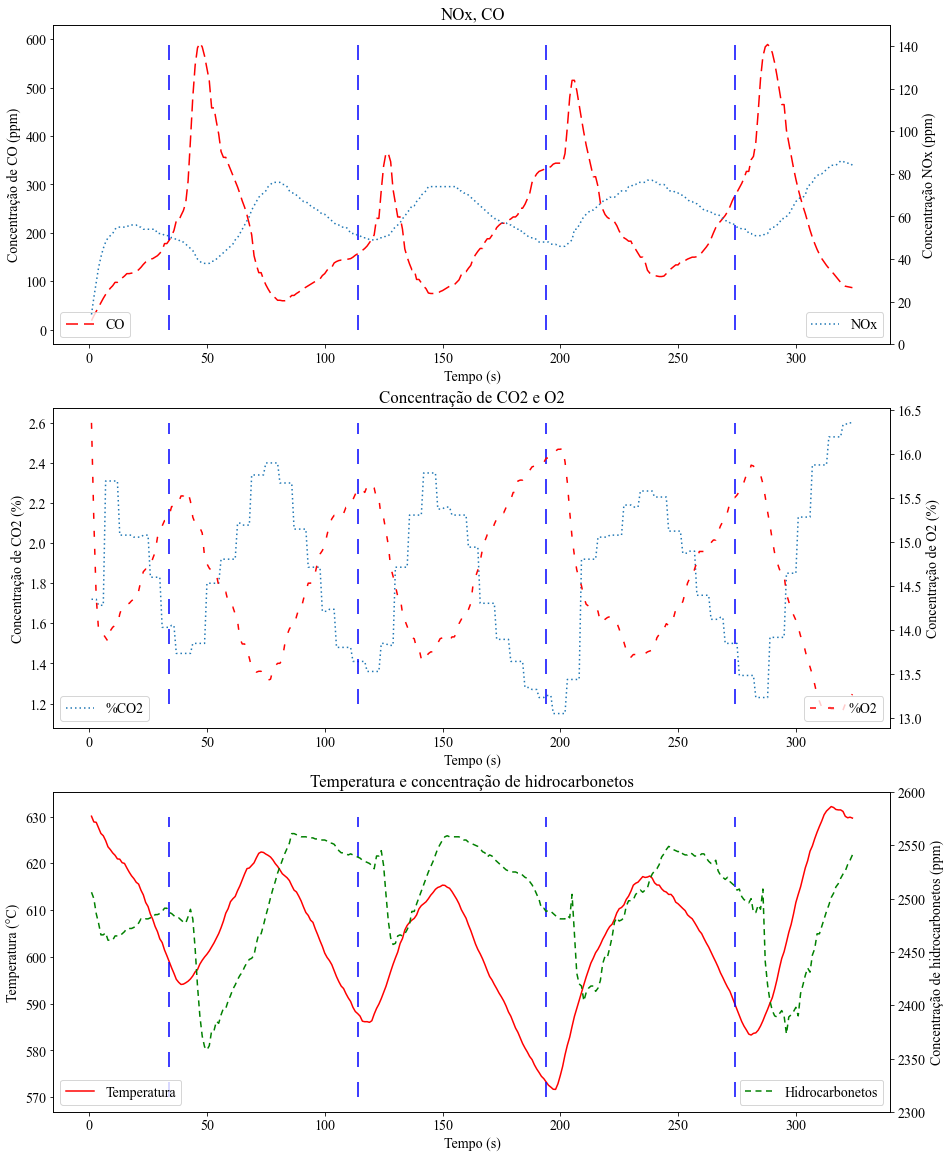
\includegraphics[scale=0.46]{Textuais/results/emissoespot3.png}}
	\fonte{O autor (2022).}
	\label{fig:emissoespot3}
\end{figure}

Do terceiro gráfico da Figura \ref{fig:emissoespot3} percebe-se que, logo após a alimentação de pellets, a temperatura tende a continuar caindo por um pequeno intervalo de tempo. Isso acontece pois a biomassa entra no reator relativamente fria e com alguma umidade, sendo necessário um certo tempo para o conjunto ganhar calor. Assim que o combustível inicia o desprendimento dos voláteis, a reação de combustão no topo do reator começa a se intensificar, o que aumenta a temperatura dos gases de combustão. Essa temperatura atinge um máximo aproximadamente na metade do intervalo $TL$. quando então começa a diminuir devido à diminuição de combustível, com consequente diminuição da volatilização e da combustão. A temperatura cai até aproximadamente o valor inicial, quando então ocorre uma nova alimentação, e o ciclo se repete.

Partindo para análise da concentração de \ch{CO} (primeiro gráfico), percebe-se que sua concentração aumenta abruptamente após o despejo da biomassa, devido justamente ao caráter transiente das reações no reator. À medida em que o tempo passa e a temperatura aumenta, a reação de formação de dióxido de carbono (concentração mostrada no segundo gráfico) é favorecida, tendo em vista que ambas as concentrações de \ch{CO} e \ch{O2} são altas. Dessa forma, a concentração de \ch{CO2} aumenta enquanto as de \ch{CO} e \ch{O2} diminuem. Verifica-se um máximo na concentração de \ch{CO2} que é bastante próximo ao ponto de máxima temperatura. Conforme o tempo passa e a quantidade de combustível disponível é menor, os níveis de \ch{CO2} diminuem, enquanto os níveis de \ch{CO} gradativamente voltam a aumentar. Um dos fatores responsáveis pela oxidação do \ch{CO} após a injeção de combustível pode ser a presença do vapor de água proveniente da secagem do combustível na reação. Turns (2013) ressalta que "[...] a oxidação de \ch{CO} é um processo relativamente lento, a menos que espécies químicas contendo hidrogênio estejam presentes. Até mesmo pequenas quantidades de \ch{H2O} ou \ch{H2} podem ter um grande efeito na taxa de oxidação". 

A concentração de $\ch{NO}_x$ registrada no primeiro gráfico varia proporcionalmente à temperatura. Tendo em vista que a formação de $\ch{NO}_x$ é favorecida com o aumento de temperatura \cite{Turns}, o resultado obtido é condizente com a literatura. 

Para as demais potências os gráficos são mostrados nas Figuras \ref{fig:emissoespot5} e \ref{fig:emissoespot7}.

\begin{figure}[!ht]
	\centering
	\caption{Emissões para a potência 5 (10,57 kW).}
	\frame{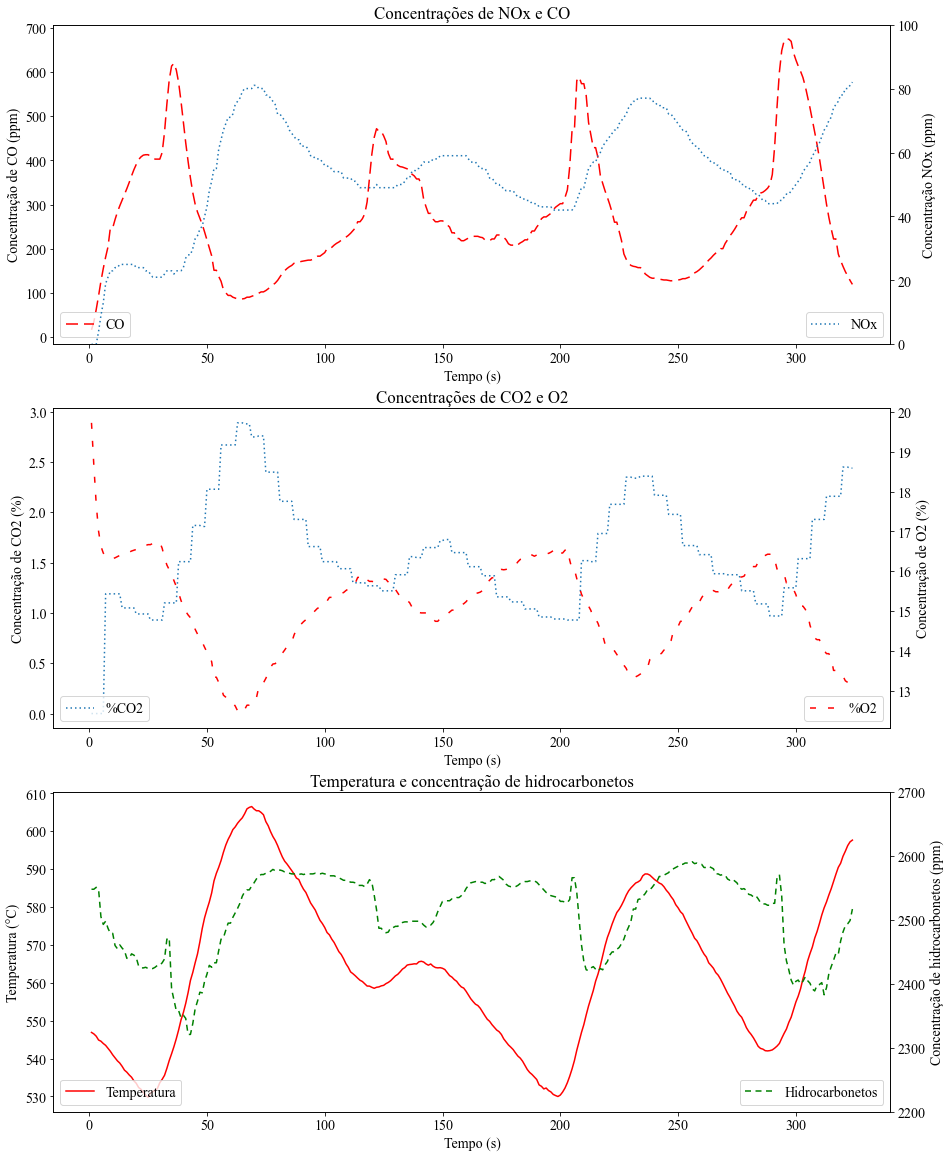
\includegraphics[scale=0.46]{Textuais/results/emissoespot5.png}}
	\fonte{O autor (2022).}
	\label{fig:emissoespot5}
\end{figure}

\begin{figure}[!ht]
	\centering
	\caption{Emissões para a potência 7 (9,63 kW).}
	\frame{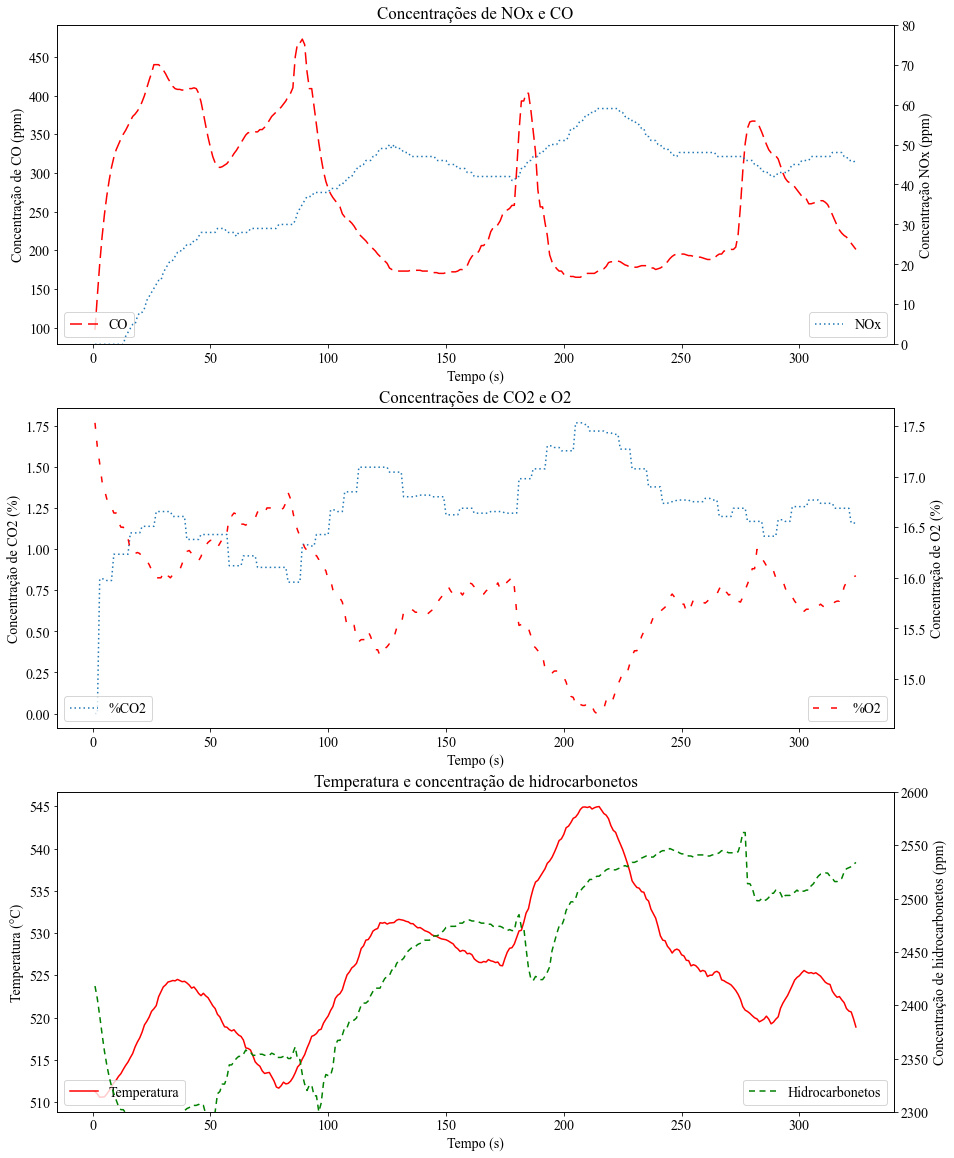
\includegraphics[scale=0.46]{Textuais/results/emissoespot7.png}}
	\fonte{O autor (2022).}
	\label{fig:emissoespot7}
\end{figure}

Nesses gráficos percebe-se que o comportamento é bastante semelhante ao já descrito para a potência de 11,42 kW. Fica evidente nos três gráficos a forte dependência da formação de $\ch{NO}_x$ com a temperatura, e também a simetria entre as curvas de \ch{CO2} e \ch{O2}. Para nenhum dos gráficos foi obtida uma conclusão precisa acerca da concentração de hidrocarbonetos, cuja oxidação é fortemente relacionada à presença de radicais O e H. 

Em termos da média nos períodos medidos, os resultados obtidos são mostrados na Tabela \ref{tab:emissoesmedias}.

\begin{table}[!htbp]
	\centering
	\small
	\renewcommand{\arraystretch}{1.3}
	\caption{Valores médios de emissões.}%
	\label{tab:emissoesmedias}
        \begin{tabular}{|l|c|c|c|}
        \hline
        \textbf{Posição do ventilador} & \textbf{7} & \textbf{5} & \textbf{3} \\ \hline
        \ch{CO} (ppm)                       & 265        & 275        & 215        \\ \hline
        $\ch{NO}_x$ (ppm)                      & 40         & 53         & 60         \\ \hline
        \ch{CO2} (\%)                    & 1,25       & 1,58       & 1,85       \\ \hline
        $C_xH_y$ (ppm)                 & 2438       & 2509       & 2494       \\ \hline
        \ch{O2} (\%)                     & 15,84      & 15,12      & 14,58      \\ \hline
        $T_{med}$ (°C)                 & 525,79     & 563,54     & 604,5      \\ \hline
        \end{tabular}
    \vspace{2mm}
	\fonte{O autor (2022).}
\end{table}

No Brasil, o CONAMA (Conselho Nacional do Meio Ambiente) regula os níveis máximos de emissão de poluentes atmosféricos para fontes fixas. A atual resolução (CONAMA 382/06) é válida para licenças de instalação requeridas após 02/01/2007, portanto será usada como base na presente análise. Para processos de geração de calor a partir da combustão externa de derivados de madeira, os limites são mostrados na Figura \ref{fig:CONAMA}.

\begin{figure}[!ht]
     \centering
        \caption{Limites para emissões de poluentes, de acordo com a Resolução CONAMA 382/06.}
        \label{fig:CONAMA}
     \begin{subfigure}[b]{0.8\linewidth}
         \centering
         \frame{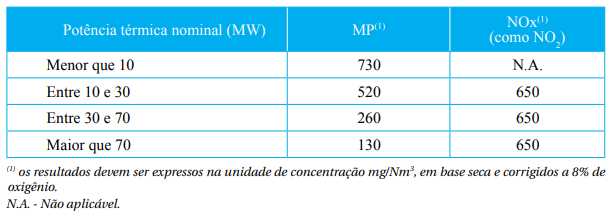
\includegraphics[width=\columnwidth]{Textuais/results/CONAMA_2.png}}
         \caption{}
         \label{fig:conama2}
     \end{subfigure}
     \hfill
     \begin{subfigure}{0.8\linewidth}
         \centering
         \frame{\includegraphics[width=\columnwidth]{Textuais/results/CONAMA_1.png}}
         \caption{}
         \label{fig:conama1}
     \end{subfigure}
     \fonte{CONAMA (2006).}
\end{figure}

\noindent A norma exige um fator de correção, dado pela Equação \eqref{eq:correcao}.
\begin{equation} \label{eq:correcao}
    C_R = \frac{21-O_R}{21-O_M} C_M
\end{equation}

\noindent Na Equação:
\begin{enumerate}
    \item $C_R$: concentração do poluente corrigida pela condição da resolução;
    \item $O_R$: porcentagem de oxigênio de referência (nesse caso 8\%);
    \item $O_M$: porcentagem de oxigênio medida durante a amostragem;
    \item $C_M$: concentração do poluente medida.
\end{enumerate}

A Tabela \ref{tab:comparacaoCONAMA} relaciona os dados de \ch{CO} obtidos no presente estudo (corrigidos a partir da Equação \eqref{eq:correcao}) com os limites requeridos pela norma. Os dados de $\ch{NO}_x$ não foram avaliados tendo em vista que a potência da aplicação é menor do que 10 MW. A conversão de ppm para $mg/Nm^3$ é realizada usando a Equação \eqref{eq:ppm}, adotando-se $MW_{CO} = 28,01$ kg/kmol.
\begin{equation} \label{eq:ppm}
    CO \left[\frac{mg}{Nm^3}\right] = CO [ppm]\cdot \frac{MW_{CO}}{22,4}
\end{equation}

\begin{table}[!htbp]
	\centering
	\small
	\renewcommand{\arraystretch}{1.3}
	\caption{Conversão dos valores obtidos no presente estudo para comparação com a Resolução.}%
	\label{tab:comparacaoCONAMA}
        \begin{tabular}{|l|c|c|c|c|}
        \hline
        \textbf{Posição do ventilador} & CO (ppm) & CO ($mg/Nm^3$) & $O_2$ (\%) & $C_{CO, R} (mg/Nm^3)$ \\ \hline
        \textbf{7}                     & 265      & 331,37            & 15,84        & 834,84                \\ \hline
        \textbf{5}                     & 275       & 343,87             & 15,12         & 760,26                \\ \hline
        \textbf{3}                     & 215     & 268,85           & 14,58       & 544,39                \\ \hline
        \end{tabular}
    \vspace{2mm}
	\fonte{O autor.}
\end{table}

Percebe-se que os valores obtidos para $C_{CO,R}$ encontram-se significativamente abaixo do limite previsto na Resolução (de 6500 $mg/Nm^3$), indicando que o equipamento atende a norma vigente de limite de emissões no Brasil. 




% -----------------------------------------------------------------
% ELEMENTOS PÓS-TEXTUAIS
% -----------------------------------------------------------------
\postextual

% Você pode comentar os elementos que não deseja em seu trabalho;
% ----------------------------------------------------------
% Glossário
% ----------------------------------------------------------

%Consulte o manual da classe abntex2 para orientações sobre o glossário.

%\glossary




% ----------------------------------------------------------
% Glossário (Formatado Manualmente)
% ----------------------------------------------------------

\chapter*{CONCLUSÃO}

%{ \setlength{\parindent}{0pt} % ambiente sem indentação
No presente trabalho um protótipo de queimador de pellets de madeira foi o objeto de estudo, buscando-se sua caracterização do ponto de vista qualitativo e quantitativo. Na revisão bibliográfica, foram analisados reatores com princípio de funcionamento semelhante ao do protótipo, e na etapa de metodologia experimental foi caracterizada a bancada experimental do projeto.

As principais conclusões obtidas no presente estudo são listadas abaixo.

\begin{itemize}
    \item O protótipo original fornecido pela empresa operava em potências muito elevadas, inviabilizando os primeiros testes, devido à potência do ventilador. Para estudos futuros, é necessária a implementação de um controlador de potência do ventilador, para um controle mais preciso do ar fornecido ao processo, e consequentemente da potência em que o queimador opera. 
    \item Para as razões de equivalência testadas, a altura da chama é inversamente proporcional à potência do queimador, devido à fluidodinâmica proporcionada pela geometria do queimador. Além disso, a chama tende a ser assimétrica em relação ao diâmetro do queimador para potências mais baixas, o que pode indicar uma influência da posição da alimentação nas variáveis analisadas.
    \item O regime permanente é caracterizado por um perfil de temperatura oscilatório, em torno de uma temperatura média constante. Quanto mais curtos os intervalos entre as alimentações de combustível, menor é a amplitude das oscilações.
    \item A emissão de poluentes é bastante relacionada ao perfil de temperatura, o que pode ser observado principalmente na Figura \ref{fig:emissoespot3}. Ainda, a concentração de cada poluente na mistura é função da concentração das demais espécies químicas.
    \item As emissões de monóxido de carbono medidas encontram-se dentro das especificações requeridas pelo CONAMA, para as potências estudadas.
\end{itemize}


O estudo aqui apresentado permite o planejamento de diversos outros ensaios para uma caracterização mais aprofundada do queimador. Dentre eles é possível citar: a determinação quantitativa da influência do intervalo de alimentação $TL$ na emissão de poluentes e no perfil da temperatura; verificação do perfil de temperatura desenvolvido ao longo da chaminé, e dentro do próprio reator, que fornece informações sobre a cinética química desenvolvida no equipamento; o estudo da influência da posição da alimentação do combustível na chama desenvolvida e nos poluentes emitidos; a implementação da análise elementar dos pellets da Koala no código do EES, visando obter condições mais fidedignas à realidade; e por fim a análise da produção de fuligem e existência de incrustações nas paredes do queimador.


%}


				% chunchei pra colocar a conclusão (que falta no template) aqui.
% Referências bibliográficas
\bibliography{abntex2-ref_UDESC_2020}	% Elemento Obrigatório

%% ----------------------------------------------------------
% Glossário
% ----------------------------------------------------------

%Consulte o manual da classe abntex2 para orientações sobre o glossário.

%\glossary




% ----------------------------------------------------------
% Glossário (Formatado Manualmente)
% ----------------------------------------------------------

\chapter*{CONCLUSÃO}

%{ \setlength{\parindent}{0pt} % ambiente sem indentação
No presente trabalho um protótipo de queimador de pellets de madeira foi o objeto de estudo, buscando-se sua caracterização do ponto de vista qualitativo e quantitativo. Na revisão bibliográfica, foram analisados reatores com princípio de funcionamento semelhante ao do protótipo, e na etapa de metodologia experimental foi caracterizada a bancada experimental do projeto.

As principais conclusões obtidas no presente estudo são listadas abaixo.

\begin{itemize}
    \item O protótipo original fornecido pela empresa operava em potências muito elevadas, inviabilizando os primeiros testes, devido à potência do ventilador. Para estudos futuros, é necessária a implementação de um controlador de potência do ventilador, para um controle mais preciso do ar fornecido ao processo, e consequentemente da potência em que o queimador opera. 
    \item Para as razões de equivalência testadas, a altura da chama é inversamente proporcional à potência do queimador, devido à fluidodinâmica proporcionada pela geometria do queimador. Além disso, a chama tende a ser assimétrica em relação ao diâmetro do queimador para potências mais baixas, o que pode indicar uma influência da posição da alimentação nas variáveis analisadas.
    \item O regime permanente é caracterizado por um perfil de temperatura oscilatório, em torno de uma temperatura média constante. Quanto mais curtos os intervalos entre as alimentações de combustível, menor é a amplitude das oscilações.
    \item A emissão de poluentes é bastante relacionada ao perfil de temperatura, o que pode ser observado principalmente na Figura \ref{fig:emissoespot3}. Ainda, a concentração de cada poluente na mistura é função da concentração das demais espécies químicas.
    \item As emissões de monóxido de carbono medidas encontram-se dentro das especificações requeridas pelo CONAMA, para as potências estudadas.
\end{itemize}


O estudo aqui apresentado permite o planejamento de diversos outros ensaios para uma caracterização mais aprofundada do queimador. Dentre eles é possível citar: a determinação quantitativa da influência do intervalo de alimentação $TL$ na emissão de poluentes e no perfil da temperatura; verificação do perfil de temperatura desenvolvido ao longo da chaminé, e dentro do próprio reator, que fornece informações sobre a cinética química desenvolvida no equipamento; o estudo da influência da posição da alimentação do combustível na chama desenvolvida e nos poluentes emitidos; a implementação da análise elementar dos pellets da Koala no código do EES, visando obter condições mais fidedignas à realidade; e por fim a análise da produção de fuligem e existência de incrustações nas paredes do queimador.


%}


				% Elemento Opcional
%
% ----------------------------------------------------------
% Apêndices
% ----------------------------------------------------------

% ---
% Inicia os apêndices
% ---
\begin{apendicesenv}

% Imprime uma página indicando o início dos apêndices
%\partapendices

% ----------------------------------------------------------
\chapter{TÍTULO}
% ----------------------------------------------------------


\end{apendicesenv}
% ---				% Elemento Opcional
%
% ----------------------------------------------------------
% Anexos
% ----------------------------------------------------------
%
% ---
% Inicia os anexos
% ---
\begin{anexosenv}

% Imprime uma página indicando o início dos anexos
%\partanexos

% ---
\chapter{TÍTULO}
% ---



\end{anexosenv}
				% Elemento Opcional
%
%%---------------------------------------------------------------------
%% INDICE REMISSIVO
%%---------------------------------------------------------------------

%\phantompart
%\printindex

%---------------------------------------------------------------------

%%---------------------------------------------------------------------
%% INDICE REMISSIVO (Formatado Manualmente)
%%---------------------------------------------------------------------

\chapter*{ÍNDICE}
\addcontentsline{toc}{chapter}{ÍNDICE}

{ \setlength{\parindent}{0pt}  % ambiente sem indentação
	
Andesito, 22, 50, 73

Argila, 52, 75, 121

Basalto, 25, 230, 235

	
	
	
	
} % fim ambiente sem indentação


		% Elemento Opcional

\end{document}

% -----------------------------------------------------------------
% Fim do Documento
% -----------------------------------------------------------------	